\documentclass[10pt,mathserif]{beamer}

\usepackage{graphicx,amsmath,amssymb,tikz,psfrag}
\usepackage{pythonhighlight, subcaption, natbib}
\usepackage{csquotes}

% ------------------------------------------------------------------------
% Packages
% ------------------------------------------------------------------------
\usepackage{amsmath}
\usepackage{tabularx}

% ------------------------------------------------------------------------
% Macros
% ------------------------------------------------------------------------
%~~~~~~~~~~~~~~~
% List shorthand
%~~~~~~~~~~~~~~~
\newcommand{\BIT}{\begin{itemize}}
\newcommand{\EIT}{\end{itemize}}
\newcommand{\BNUM}{\begin{enumerate}}
\newcommand{\ENUM}{\end{enumerate}}
%~~~~~~~~~~~~~~~
% Text with quads around it
%~~~~~~~~~~~~~~~
\newcommand{\qtext}[1]{\quad\text{#1}\quad}
%~~~~~~~~~~~~~~~
% Shorthand for math formatting
%~~~~~~~~~~~~~~~
\newcommand\mbb[1]{\mathbb{#1}}
\newcommand\mbf[1]{\mathbf{#1}}
\def\mc#1{\mathcal{#1}}
\def\mrm#1{\mathrm{#1}}
%~~~~~~~~~~~~~~~
% Common sets
%~~~~~~~~~~~~~~~
\def\reals{\mathbb{R}} % Real number symbol
\def\integers{\mathbb{Z}} % Integer symbol
\def\rationals{\mathbb{Q}} % Rational numbers
\def\naturals{\mathbb{N}} % Natural numbers
\def\complex{\mathbb{C}} % Complex numbers
\def\simplex{\mathcal{S}} % Simplex
%~~~~~~~~~~~~~~~
% Common functions
%~~~~~~~~~~~~~~~
\renewcommand{\exp}[1]{\operatorname{exp}\left(#1\right)} % Exponential
\def\indic#1{\mbb{I}\left({#1}\right)} % Indicator function
\providecommand{\maximize}{\mathop\mathrm{maximize}} % Defining math symbols
\providecommand{\minimize}{\mathop\mathrm{minimize}}
\providecommand{\argmax}{\mathop\mathrm{arg max}}
\providecommand{\argmin}{\mathop\mathrm{arg min}}
\providecommand{\arccos}{\mathop\mathrm{arccos}}
\providecommand{\asinh}{\mathop\mathrm{asinh}}
\providecommand{\dom}{\mathop\mathrm{dom}} % Domain
\providecommand{\range}{\mathop\mathrm{range}} % Range
\providecommand{\diag}{\mathop\mathrm{diag}}
\providecommand{\tr}{\mathop\mathrm{tr}}
\providecommand{\abs}{\mathop\mathrm{abs}}
\providecommand{\card}{\mathop\mathrm{card}}
\providecommand{\sign}{\mathop\mathrm{sign}}
\def\rank#1{\mathrm{rank}({#1})}
\def\supp#1{\mathrm{supp}({#1})}
%~~~~~~~~~~~~~~~
% Common probability symbols
%~~~~~~~~~~~~~~~
\def\E{\mathbb{E}} % Expectation symbol
\def\Earg#1{\E\left[{#1}\right]}
\def\Esubarg#1#2{\E_{#1}\left[{#2}\right]}
\def\P{\mathbb{P}} % Probability symbol
\def\Parg#1{\P\left({#1}\right)}
\def\Psubarg#1#2{\P_{#1}\left[{#2}\right]}
\def\Cov{\mrm{Cov}} % Covariance symbol
\def\Corr{\mrm{Corr}} % Covariance symbol
\def\Covarg#1{\Cov\left[{#1}\right]}
\def\Covsubarg#1#2{\Cov_{#1}\left[{#2}\right]}
\def\Corrsubarg#1#2{\Corr_{#1}\left[{#2}\right]}
\def\Var{\mrm{Var}}
\def\Vararg#1{\Var\left(#1\right)}
\def\Varsubarg#1#2{\Var_{#1}\left(#2\right)}
\newcommand{\family}{\mathcal{P}} % probability family
\newcommand{\eps}{\epsilon}
\def\absarg#1{\left|#1\right|}
\def\msarg#1{\left(#1\right)^{2}}
\def\logarg#1{\log\left(#1\right)}
%~~~~~~~~~~~~~~~
% Distributions
%~~~~~~~~~~~~~~~
\def\Gsn{\mathcal{N}}
\def\Ber{\textnormal{Ber}}
\def\Bin{\textnormal{Bin}}
\def\Unif{\textnormal{Unif}}
\def\Mult{\textnormal{Mult}}
\def\Cat{\textnormal{Cat}}
\def\Gam{\textnormal{Gam}}
\def\InvGam{\textnormal{InvGam}}
\def\NegMult{\textnormal{NegMult}}
\def\Dir{\textnormal{Dir}}
\def\Lap{\textnormal{Laplace}}
\def\Bet{\textnormal{Beta}}
\def\Poi{\textnormal{Poi}}
\def\HypGeo{\textnormal{HypGeo}}
\def\GEM{\textnormal{GEM}}
\def\BP{\textnormal{BP}}
\def\DP{\textnormal{DP}}
\def\BeP{\textnormal{BeP}}
%~~~~~~~~~~~~~~~
% Theorem-like environments
%~~~~~~~~~~~~~~~

%-----------------------
% Probability sets
%-----------------------
\newcommand{\X}{\mathcal{X}}
\newcommand{\Y}{\mathcal{Y}}
\newcommand{\D}{\mathcal{D}}
\newcommand{\Scal}{\mathcal{S}}
%-----------------------
% vector notation
%-----------------------
\newcommand{\bx}{\mathbf{x}}
\newcommand{\by}{\mathbf{y}}
\newcommand{\bt}{\mathbf{t}}
\newcommand{\xbar}{\overline{x}}
\newcommand{\Xbar}{\overline{X}}
\newcommand{\tolaw}{\xrightarrow{\mathcal{L}}}
\newcommand{\toprob}{\xrightarrow{\mathbb{P}}}
\newcommand{\laweq}{\overset{\mathcal{L}}{=}}
\newcommand{\F}{\mathcal{F}}


\mode<presentation>
{
\usetheme{default}
}
\setbeamertemplate{navigation symbols}{}
\usecolortheme[rgb={0.13,0.28,0.59}]{structure}
\setbeamertemplate{itemize subitem}{--}
\setbeamertemplate{frametitle} {
	\begin{center}
	  {\large\bf \insertframetitle}
	\end{center}
}

\AtBeginSection[]
{
	\begin{frame}<beamer>
		\frametitle{Outline}
		\tableofcontents[currentsection,currentsubsection]
	\end{frame}
}

%% begin presentation

\title{\large \bfseries Deep Learning Foundations}
\author{Kris Sankaran\\[3ex] Nepal Winter School in AI}

\date{\today}

\begin{document}
\maketitle

\section{Introduction}
\label{sec:introduction}

\begin{frame}
  \frametitle{Deep Learning and Poetry}
  \begin{itemize}
  \item Algorithms and words are only as remarkable as human creativity
    \begin{itemize}
    \item Discover patterns and make connections unseen by others
    \end{itemize}
  \item Knowing SGD is like knowing meter
  \item I want to teach you the form, so you can write the poetry
  \end{itemize}
  \begin{figure}[ht]
    \centering
    \includegraphics[width=0.45\paperwidth]{figure/cheerios}
\end{figure}
\end{frame}

\begin{frame}
  \frametitle{Learning Objectives}
  \begin{itemize}
    \item Understand goals of deep learning, especially representation learning
    \item Logistic Regression to Backpropagation: Learn the modular-components
      view of deep learning
    \item Learn tricks for doing (and debugging) deep learning % don't pray to random number generators
    \item How to study deep learning algorithms: toy examples,
      drawing pictures, ...
  \end{itemize}
\end{frame}

\begin{frame}
  \frametitle{Ask Questions}
  \begin{displayquote}
    Truth emerges more readily from error than from confusion.
  \end{displayquote}
  Francis Bacon
  (as cited in \citep{diaconis1985theories})
\end{frame}

\begin{frame}
  \frametitle{Flipping Coins}
  \begin{itemize}
  \item Imagine $n$ flips of a coin with probability $\pi$ of coming up heads.
  \item Loglikelihood function (independent bernoulli trials)
    \begin{align*}
      \log p\left(y \vert \pi \right) &= \log \left[\prod_{i = 1}^{n} \pi^{\indic{y_i = 1}}\left(1 - \pi\right)^{\indic{y_i = 0}}\right] \\
      &= \sum_{i = 1}^{n} \indic{y_i = 1}\log \pi + \indic{y_i = 0}\log\left(1 - \pi\right)
    \end{align*}
    where we use the shorthand $y = \left(y_1, \dots, y_n\right)$.
  \end{itemize}
  \begin{figure}[ht]
    \centering
    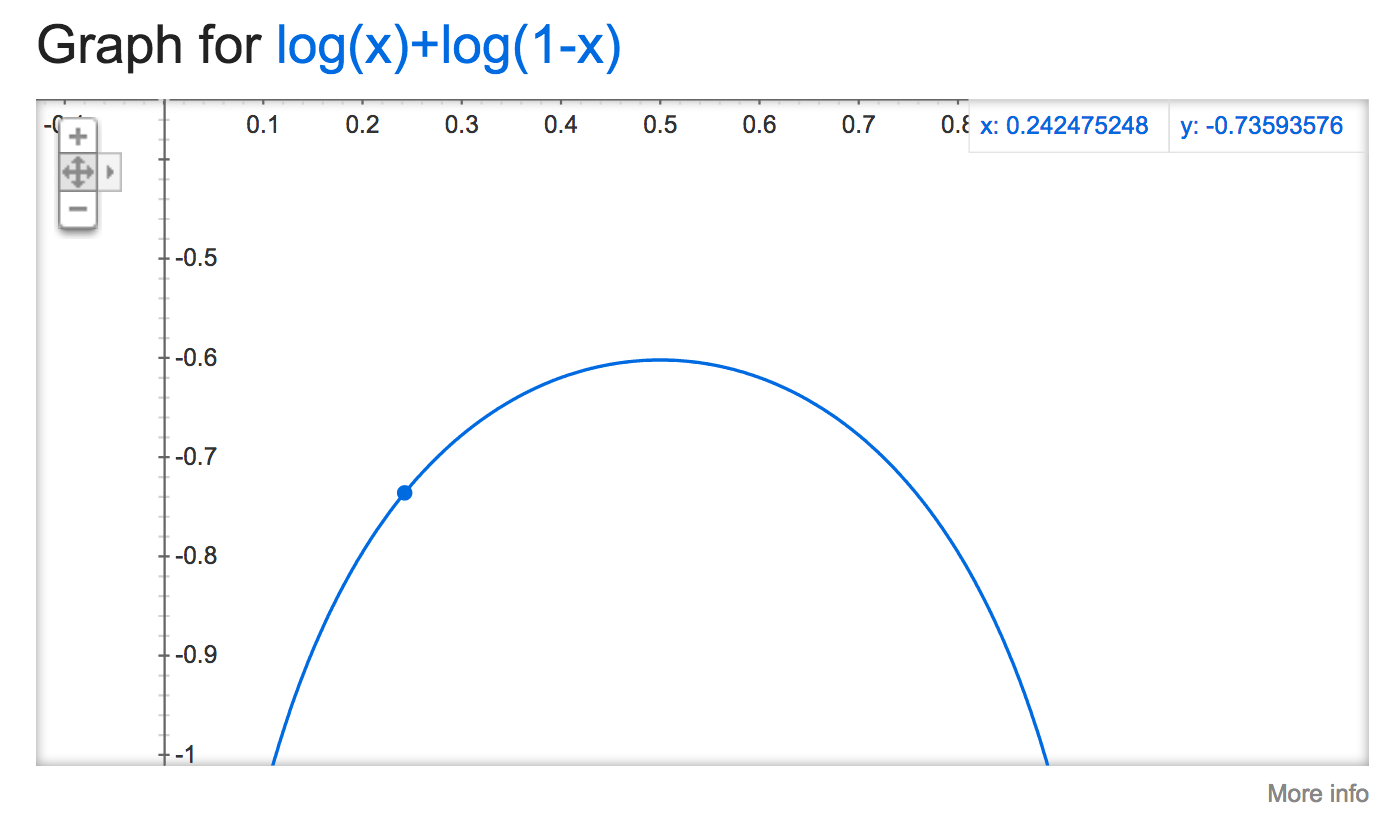
\includegraphics[width=0.3\paperwidth]{figure/loglikelihood_bernoulli}
    \caption{Logliklihoods over $\pi$ when we see one head and one tail. Seems
      most likely that $\pi \approx 0.5$. \label{fig:loglikelihood_bernoulli} }
  \end{figure}
\end{frame}

\begin{frame}
  \frametitle{Flipping Coins}
  \begin{itemize}
  \item Imagine $n$ flips of a coin with probability $\pi$ of coming up heads.
  \item Loglikelihood function (independent bernoulli trials)
    \begin{align*}
      \log p\left(y \vert \pi \right) &= \log \left[\prod_{i = 1}^{n} \pi^{\indic{y_i = 1}}\left(1 - \pi\right)^{\indic{y_i = 0}}\right] \\
      &= \sum_{i = 1}^{n} \indic{y_i = 1}\log \pi + \indic{y_i = 0}\log\left(1 - \pi\right)
    \end{align*}
    where we use the shorthand $y = \left(y_1, \dots, y_n\right)$.
  \end{itemize}
  \begin{figure}[ht]
    \centering
    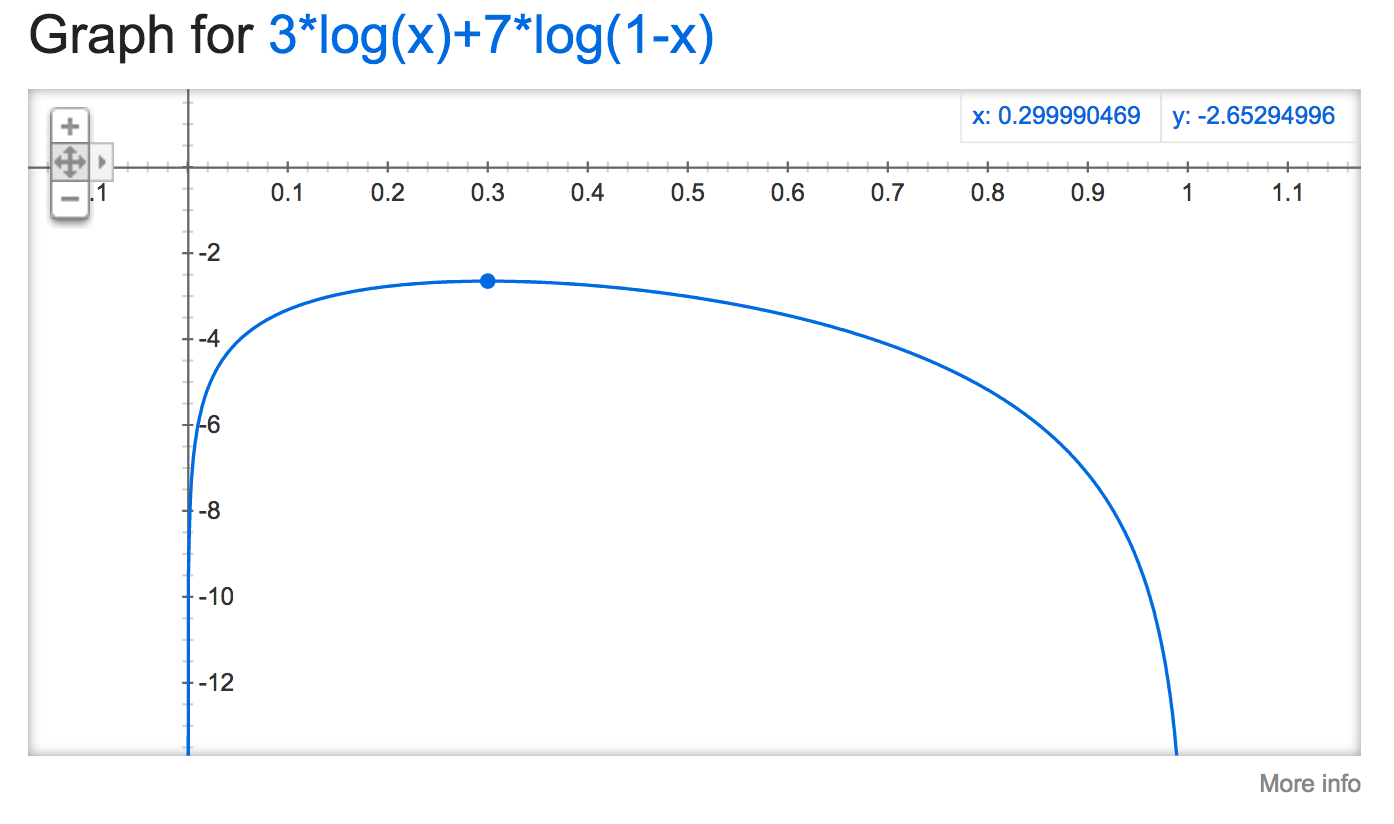
\includegraphics[width=0.3\paperwidth]{figure/loglikelihood_bernoulli_10}
    \caption{Logliklihoods over $\pi$ when we see 3 heads and 7 tails. Seems
      most likely that $\pi \approx 0.3$. \label{fig:loglikelihood_bernoulli_10} }
  \end{figure}
\end{frame}

\begin{frame}
  \frametitle{Flipping Coins}
  \begin{itemize}
  \item Imagine $n$ flips of a coin with probability $\pi$ of coming up heads.
  \item Loglikelihood function (independent bernoulli trials)
    \begin{align*}
      \log p\left(y \vert \pi \right) &= \log \left[\prod_{i = 1}^{n} \pi^{\indic{y_i = 1}}\left(1 - \pi\right)^{\indic{y_i = 0}}\right] \\
      &= \sum_{i = 1}^{n} \indic{y_i = 1}\log \pi + \indic{y_i = 0}\log\left(1 - \pi\right)
    \end{align*}
    where we use the shorthand $y = \left(y_1, \dots, y_n\right)$.
  \end{itemize}
  \begin{figure}[ht]
    \centering
    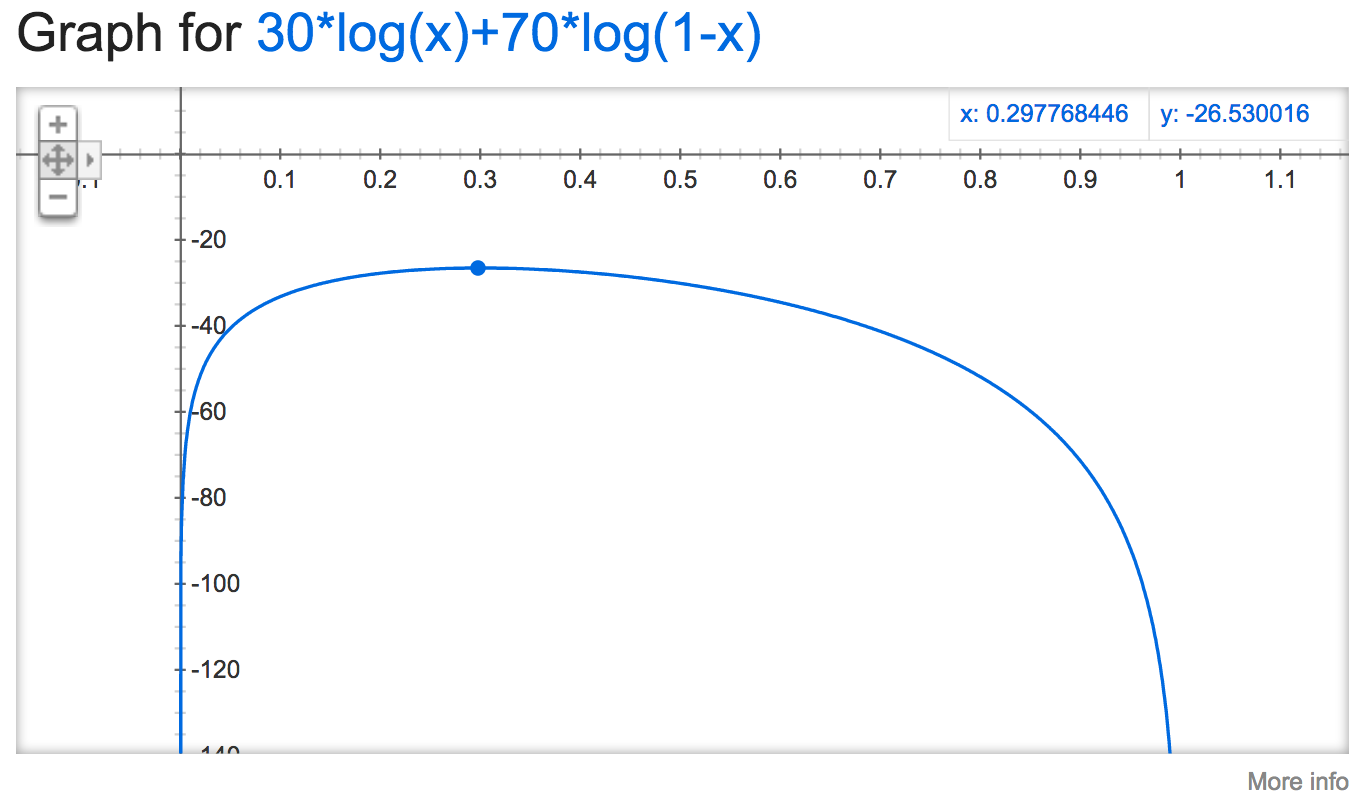
\includegraphics[width=0.3\paperwidth]{figure/loglikelihood_bernoulli_100}
    \caption{Logliklihoods over $\pi$ when we see 30 heads and 70 tails. Again seems
      most likely that $\pi \approx 0.3$, but everything is scaled by $10
      \times$. \label{fig:loglikelihood_bernoulli_100} }
  \end{figure}
\end{frame}

%% \begin{frame}
%%   \frametitle{Flipping Coins}
%%   \begin{itemize}
%%   \item Imagine $n$ flips of a coin with probability $\pi$ of coming up heads.
%%   \item Entropy function
%%     \begin{align*}
%%       -\Esubarg{p}{\log p\left(x\right)} &= \sum_{i = 1}^{n} \Esubarg{p}{\indic{x_i = 1}}\log\pi + \Esubarg{p}{x_i = 0}\left(1 - \pi\right) \\
%%       &= n \left[\pi\log\pi + \left(1 - \pi\right)\log\left(1 - \pi\right)\right]
%%     \end{align*}
%%   \end{itemize}
%% \end{frame}

\begin{frame}
  \frametitle{Using Input Data}
  \begin{itemize}
  \item What if the probability depended on input data?
  \item Depending on some input $x_i$, we have probability $\pi\left(x_i\right)$
    of heads
  \end{itemize}
  \begin{figure}
    \centering
    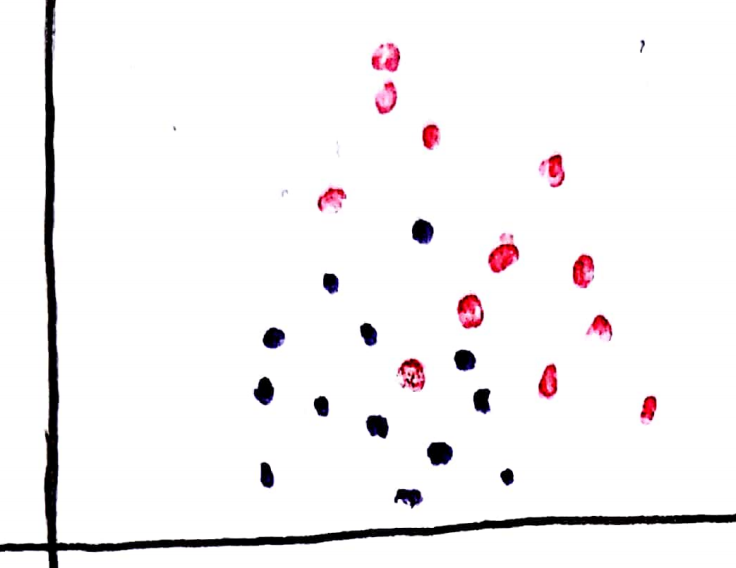
\includegraphics[width=0.3\paperwidth]{figure/logistic_scatter}
    \caption{Example of a classification problem when $x_i$ are two dimensional,
      heads are green, and tails are red. \label{fig:logistic_scatter} }
  \end{figure}
\end{frame}

\begin{frame}
  \frametitle{Using Input Data}
  \begin{itemize}
  \item What if the probability depended on input data?
  \item Depending on some input $x_i$, we have probability $\pi\left(x_i\right)$
    of heads
  \end{itemize}
  \begin{figure}
    \centering
    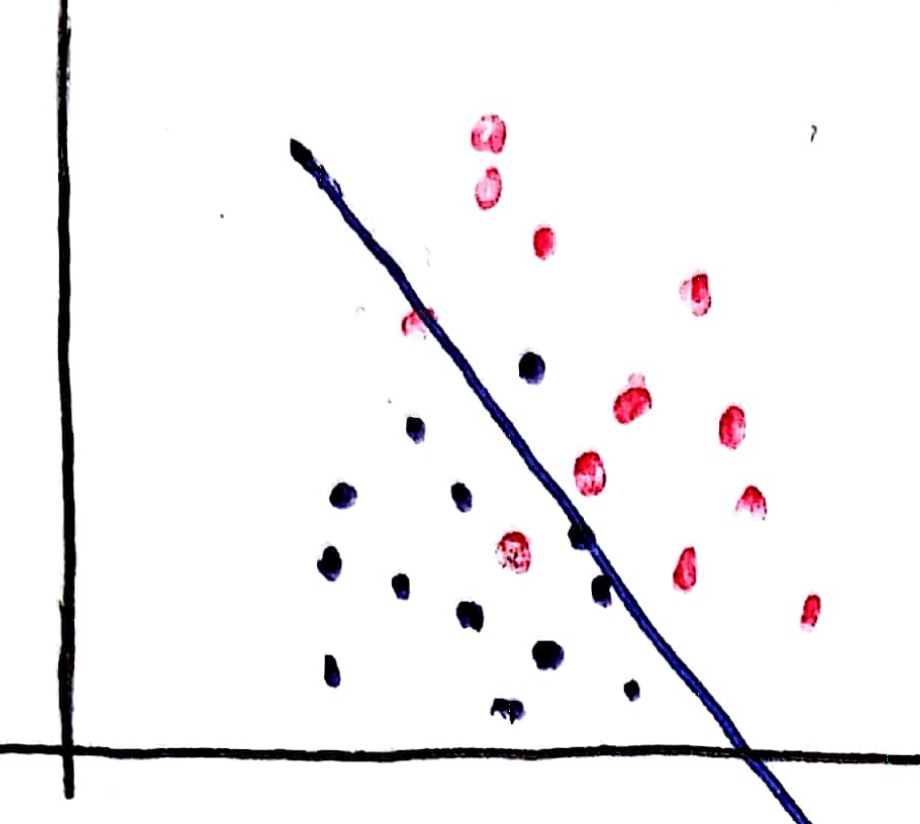
\includegraphics[width=0.3\paperwidth]{figure/logistic_scatter_plane}
    \caption{Example of a classification problem when $x_i$ are two dimensional,
      heads are green, and tails are red. \label{fig:logistic_scatter} }
  \end{figure}
\end{frame}

\begin{frame}
  \frametitle{Using Input Data}
  \begin{itemize}
  \item What if the probability depended on input data?
  \item Depending on some input $x_i$, we have probability $\pi\left(x_i\right)$
    of heads
  \end{itemize}
  \begin{figure}
    \centering
    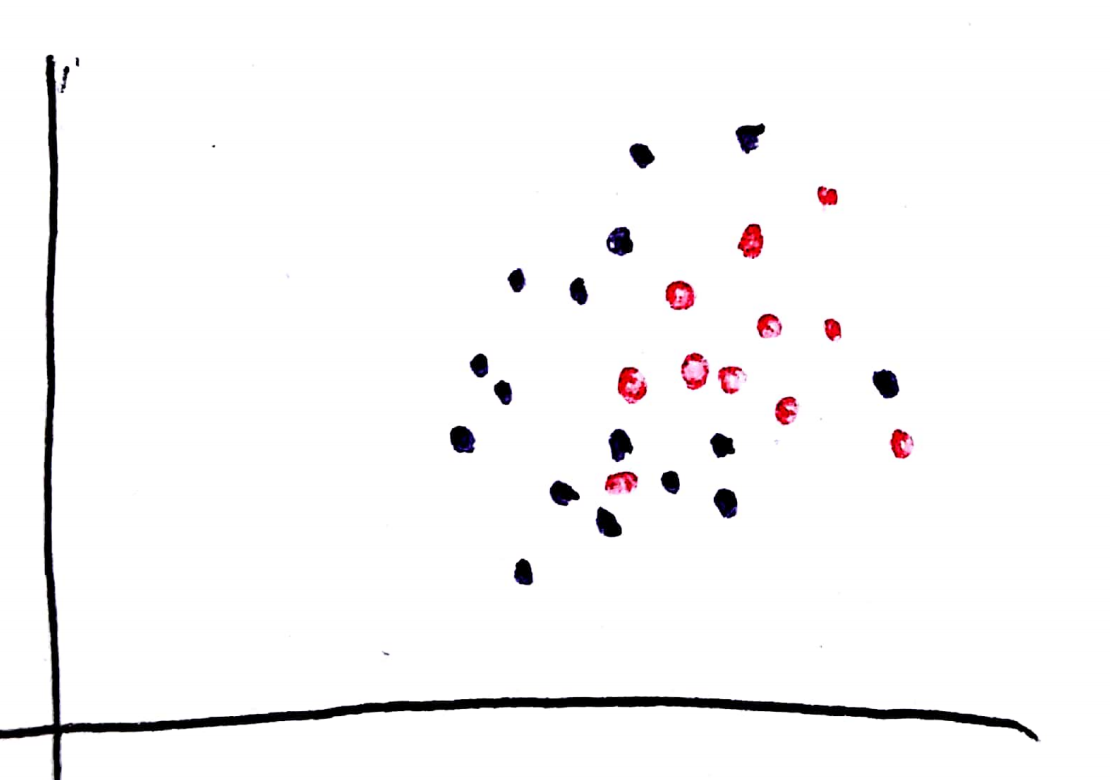
\includegraphics[width=0.45\paperwidth]{figure/logistic_scatter_nonlinear_points}
    \caption{Example with a nonlinear
      boundary. \label{fig:logistic_nonlinear_scatter_points} }
  \end{figure}
\end{frame}

\begin{frame}
  \frametitle{Using Input Data}
  \begin{itemize}
  \item What if the probability depended on input data?
  \item Depending on some input $x_i$, we have probability $\pi\left(x_i\right)$
    of heads
  \end{itemize}
  \begin{figure}
    \centering
    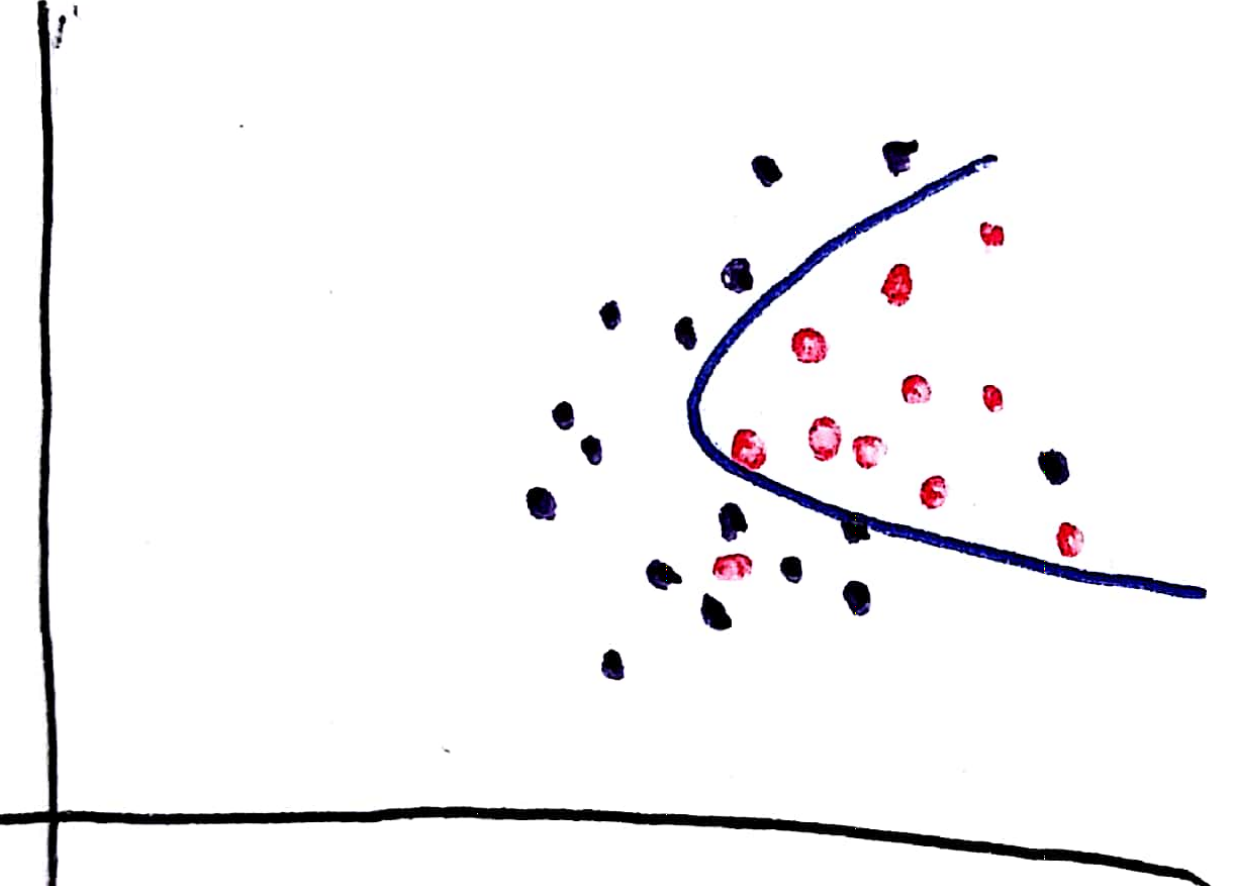
\includegraphics[width=0.45\paperwidth]{figure/logistic_scatter_nonlinear}
    \caption{Example with a nonlinear
      boundary. \label{fig:logistic_nonlinear_scatter_points} }
  \end{figure}
\end{frame}

\begin{frame}
  \frametitle{Using Input Data}
  \begin{itemize}
  \item Can adapt previous loglikelihood to this setting
    \begin{align*}
      \log p\left(y \vert x\right) &= \sum_{i = 1}^{n} \indic{y_i = 1}\log \pi\left(x\right) + \indic{y_i = 0}\log\left(1 - \pi\left(x\right)\right)
    \end{align*}
  \item Need to learn $\pi\left(x\right)$, just like we learned $\pi$ before
  \end{itemize}
\end{frame}

\begin{frame}
  \frametitle{Sigmoid Function}
  \begin{itemize}
  \item Consider the collection of functions (one for each $\theta$)
    \begin{align*}
      \pi_{\theta}\left(x\right) &= \frac{1}{1 + \exp{-\theta^{T}x}} \stackrel{\text{defined}}{=}\sigma\left(\theta^{T}x\right)
    \end{align*}
  \end{itemize}
  \begin{figure}
    \begin{subfigure}{.17\paperwidth}
      \centering
      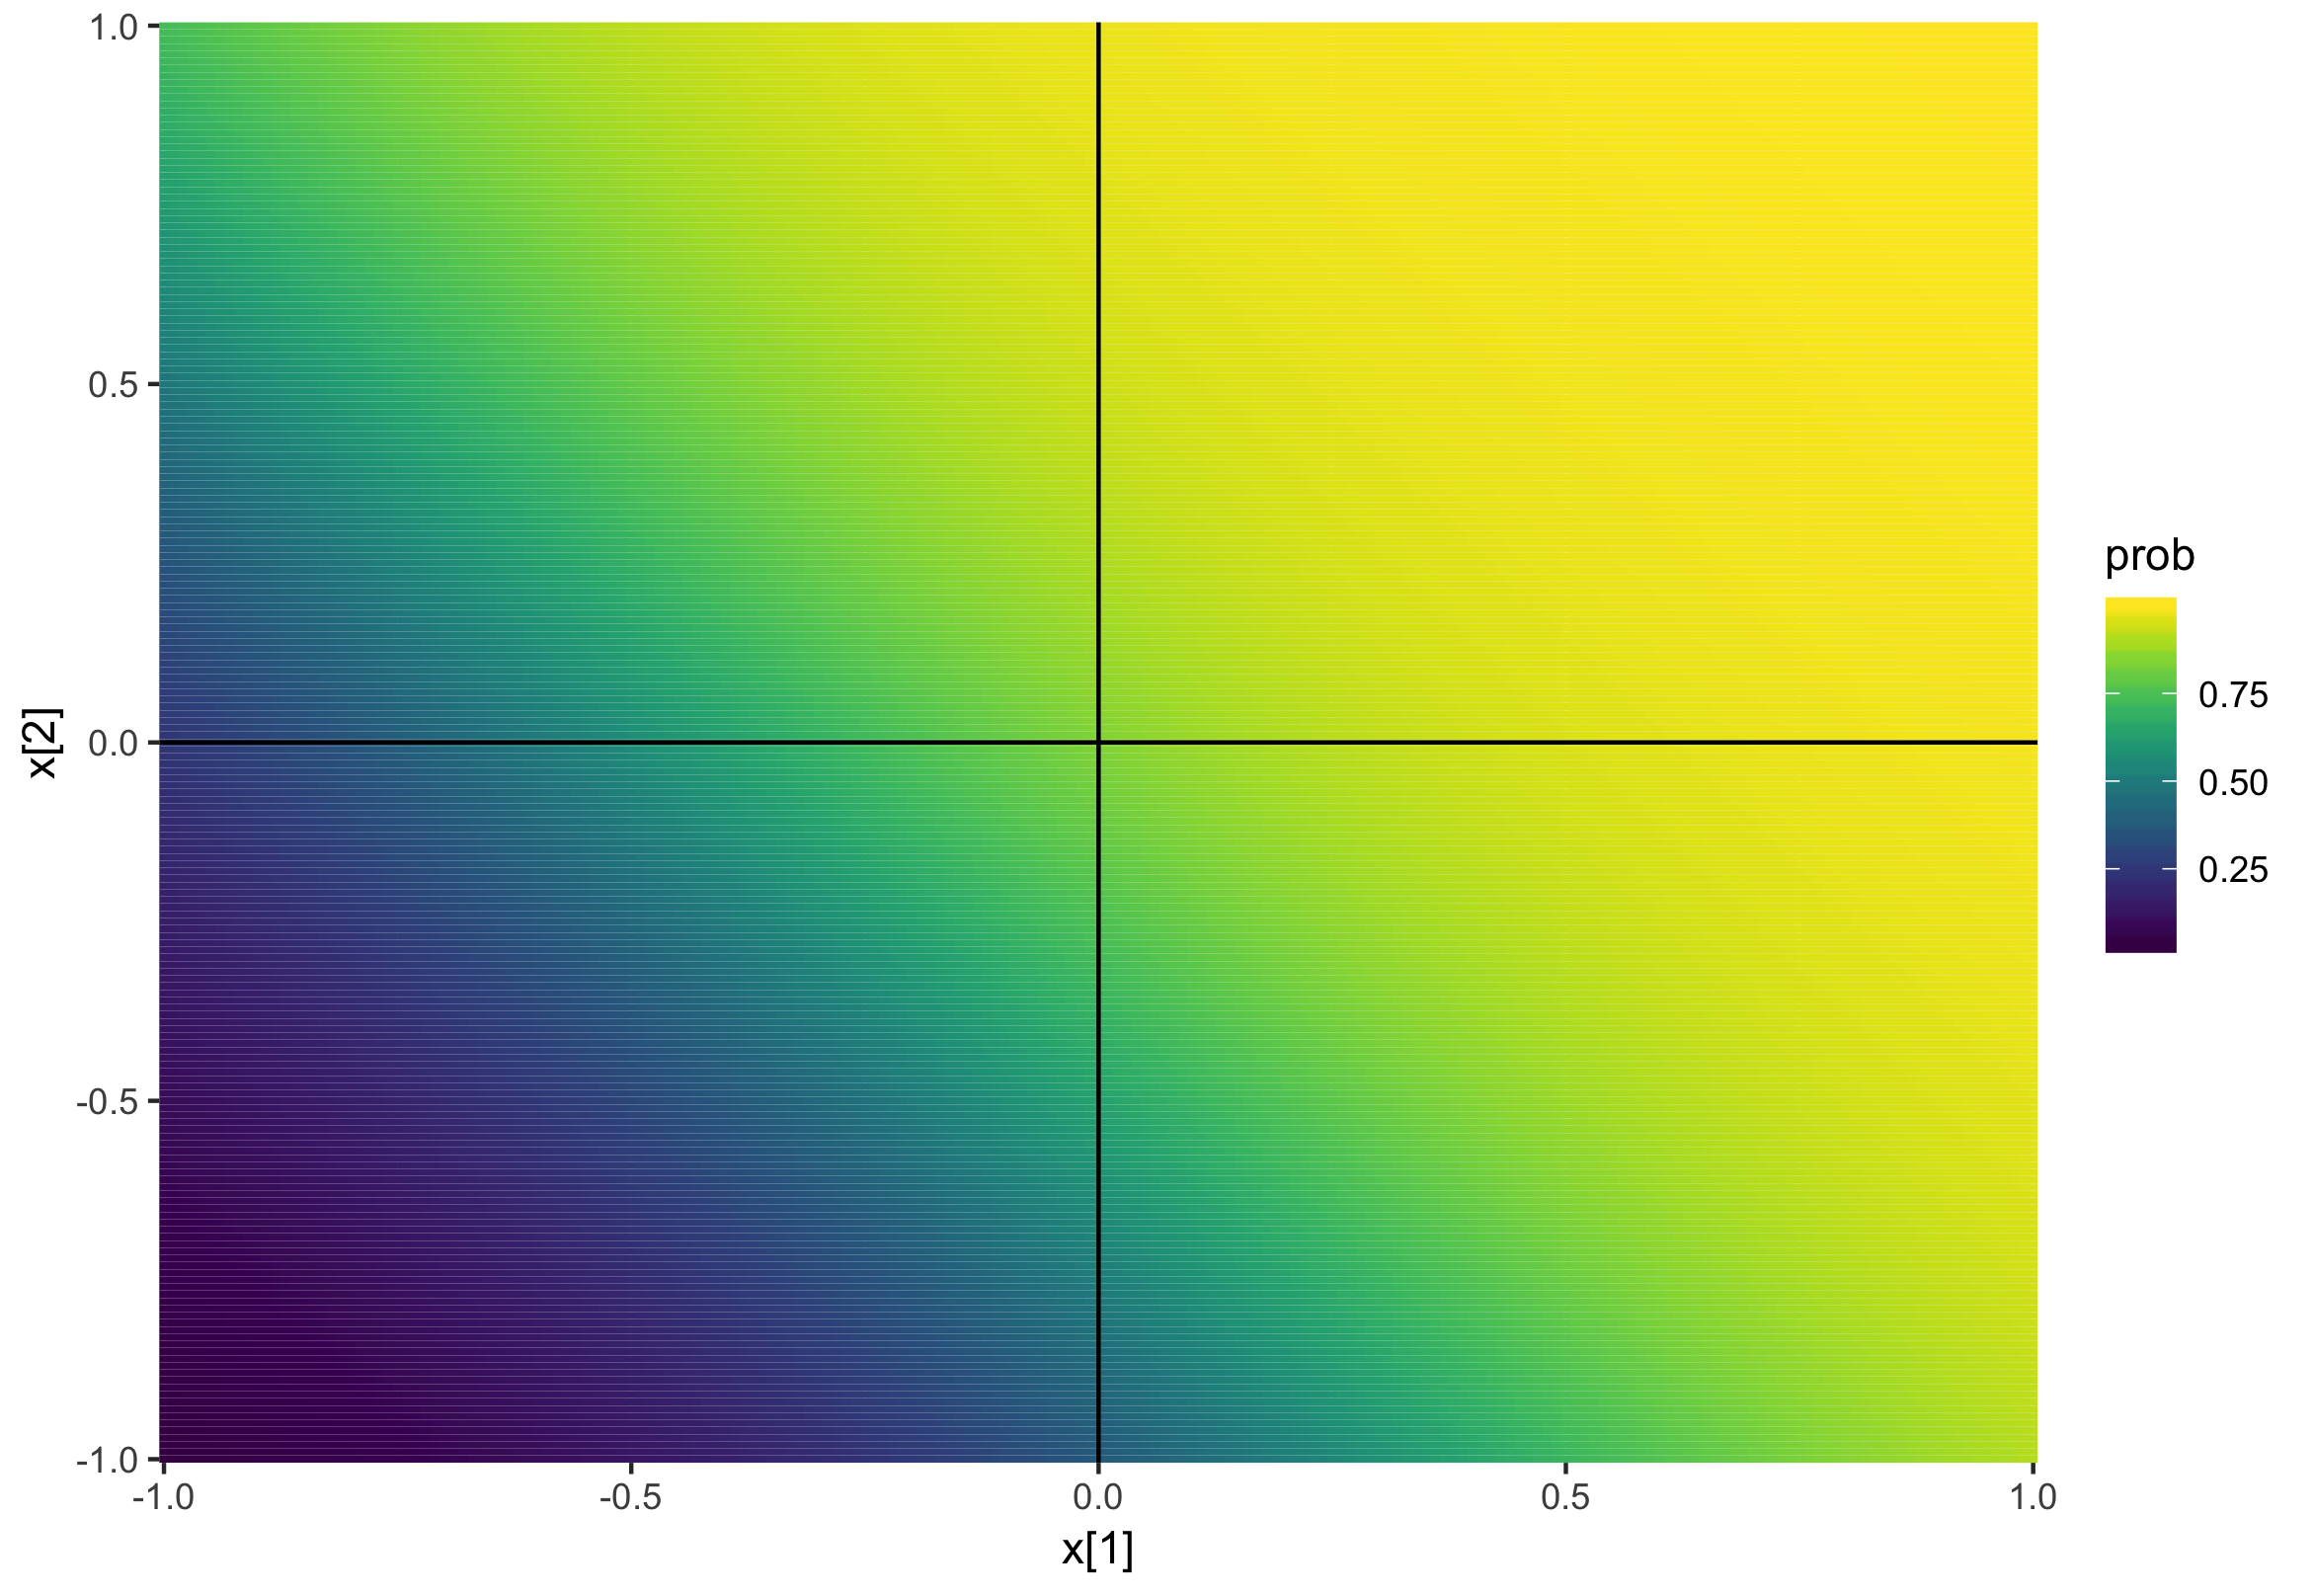
\includegraphics[width=0.17\paperwidth]{figure/sigmoid_plot_1}
    \end{subfigure}
    \begin{subfigure}{.17\paperwidth}
      \centering
      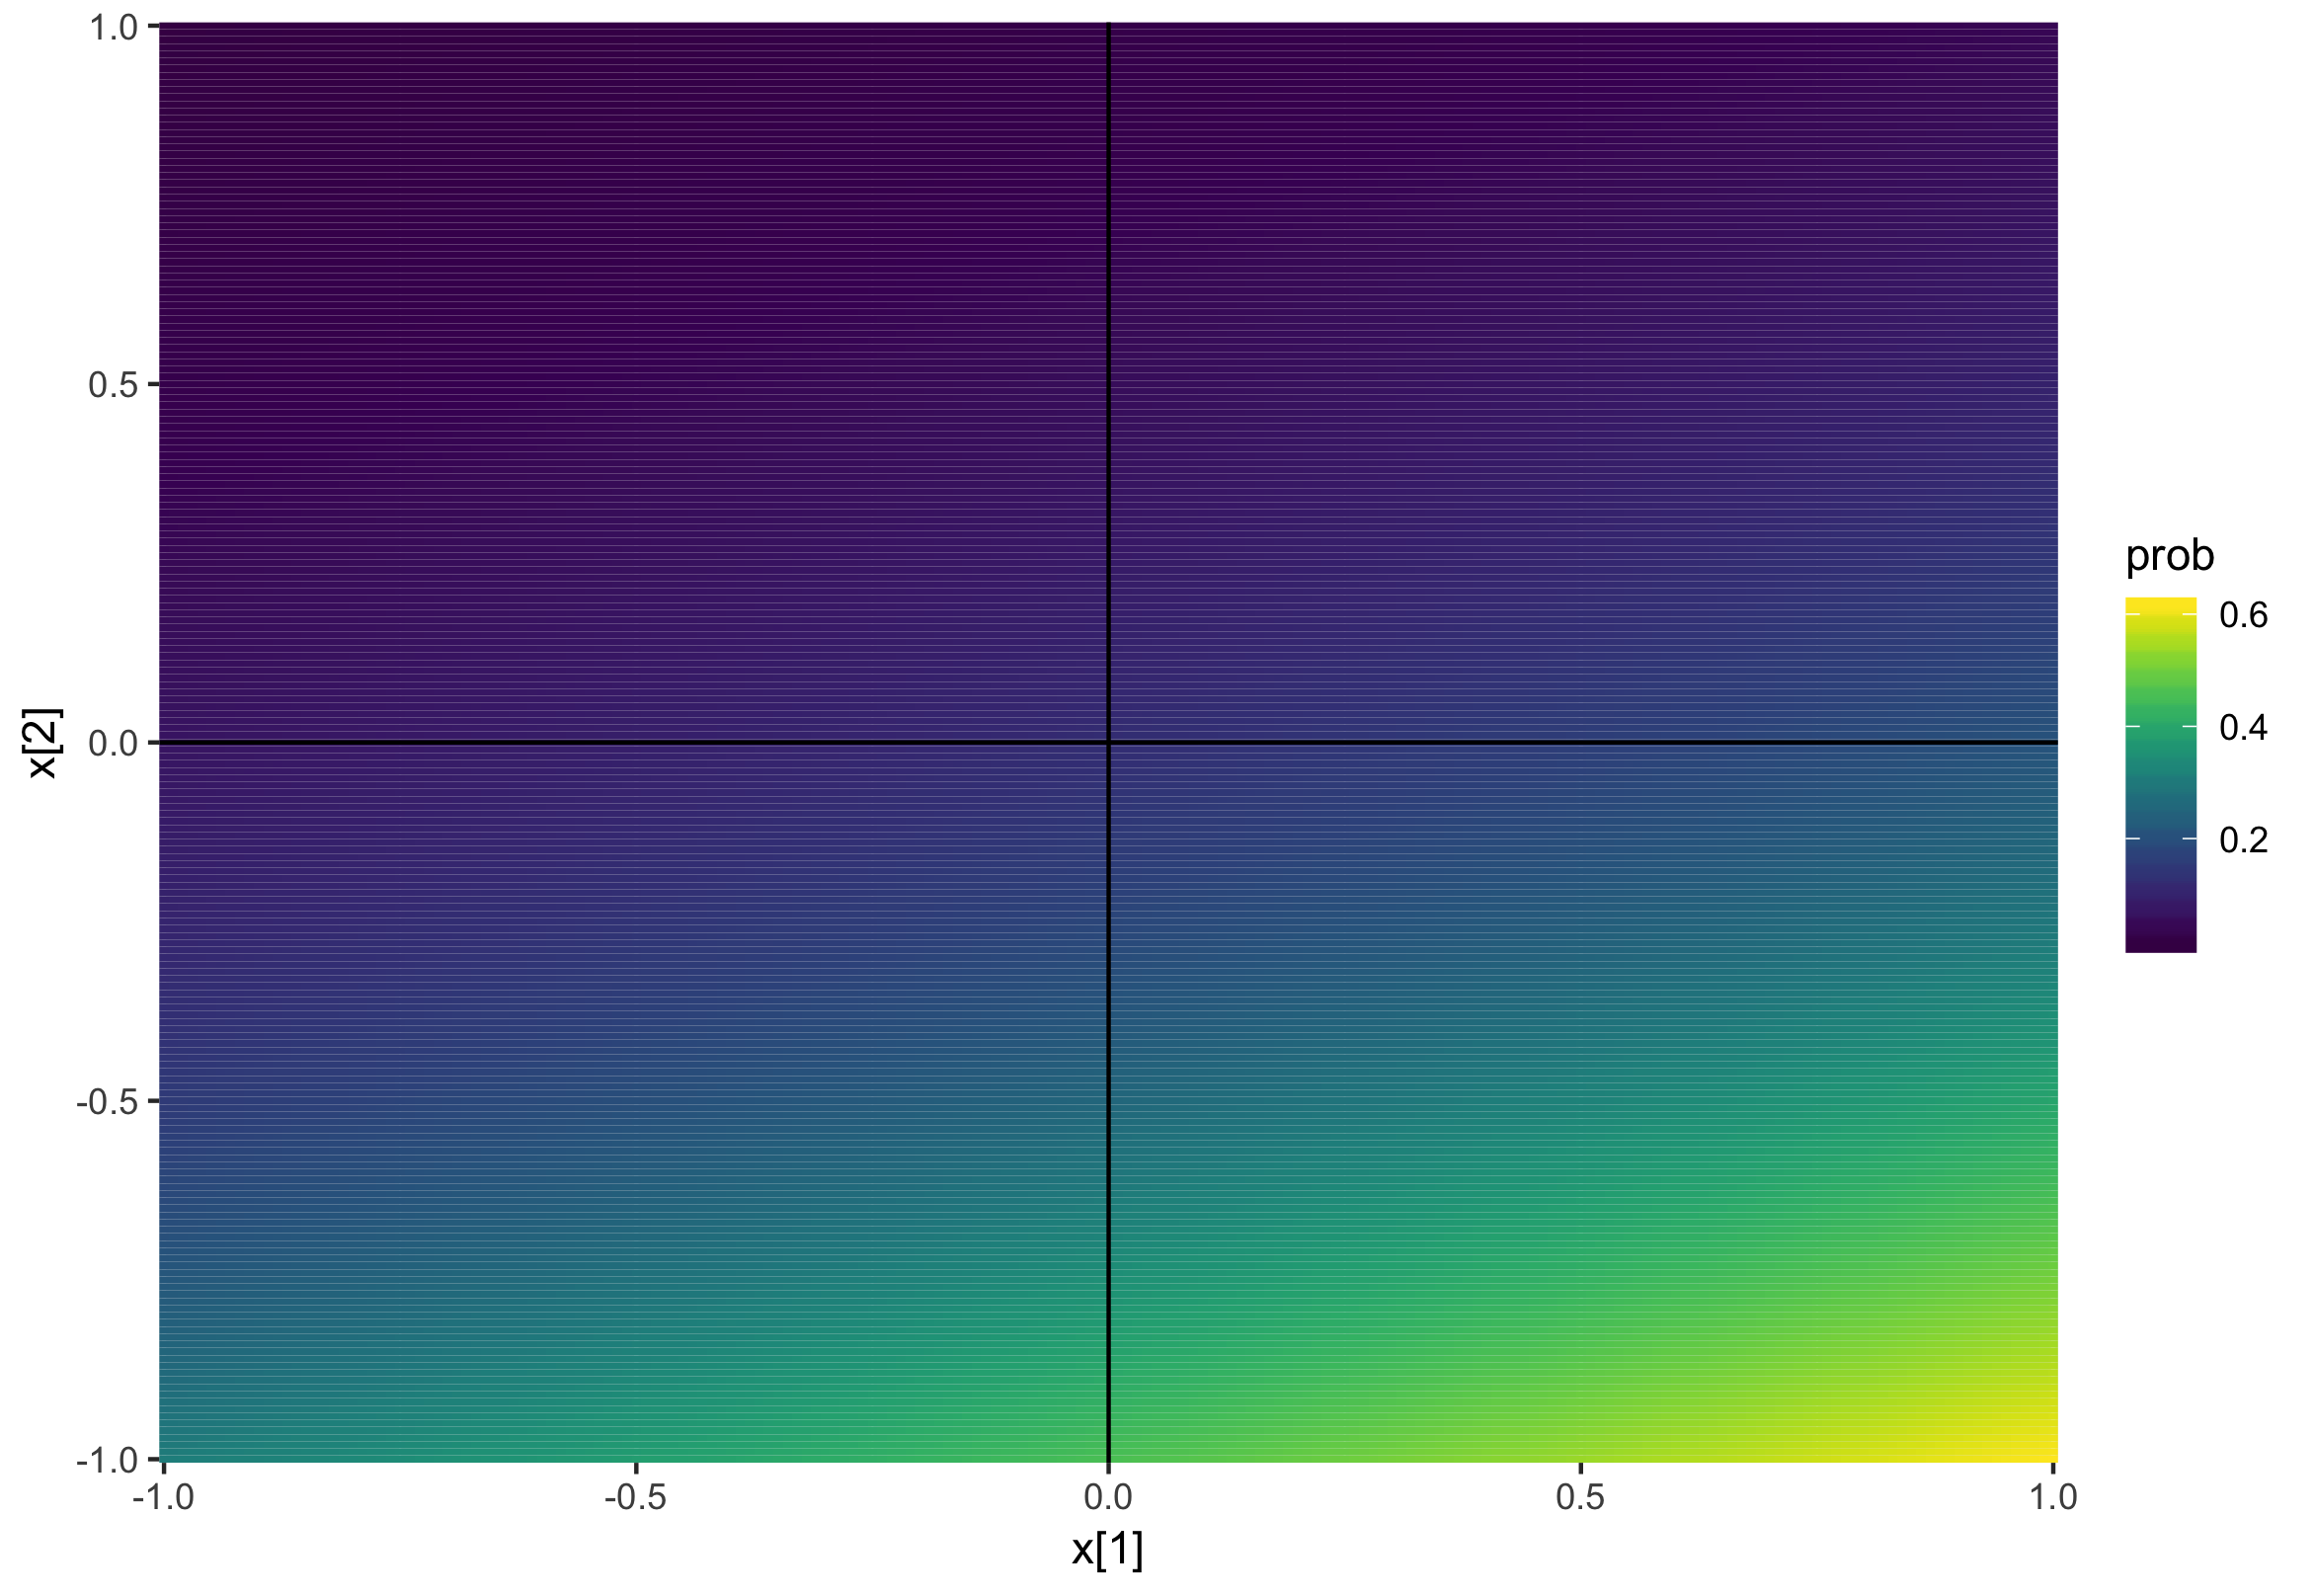
\includegraphics[width=0.17\paperwidth]{figure/sigmoid_plot_2}
    \end{subfigure}
    \begin{subfigure}{.17\paperwidth}
      \centering
      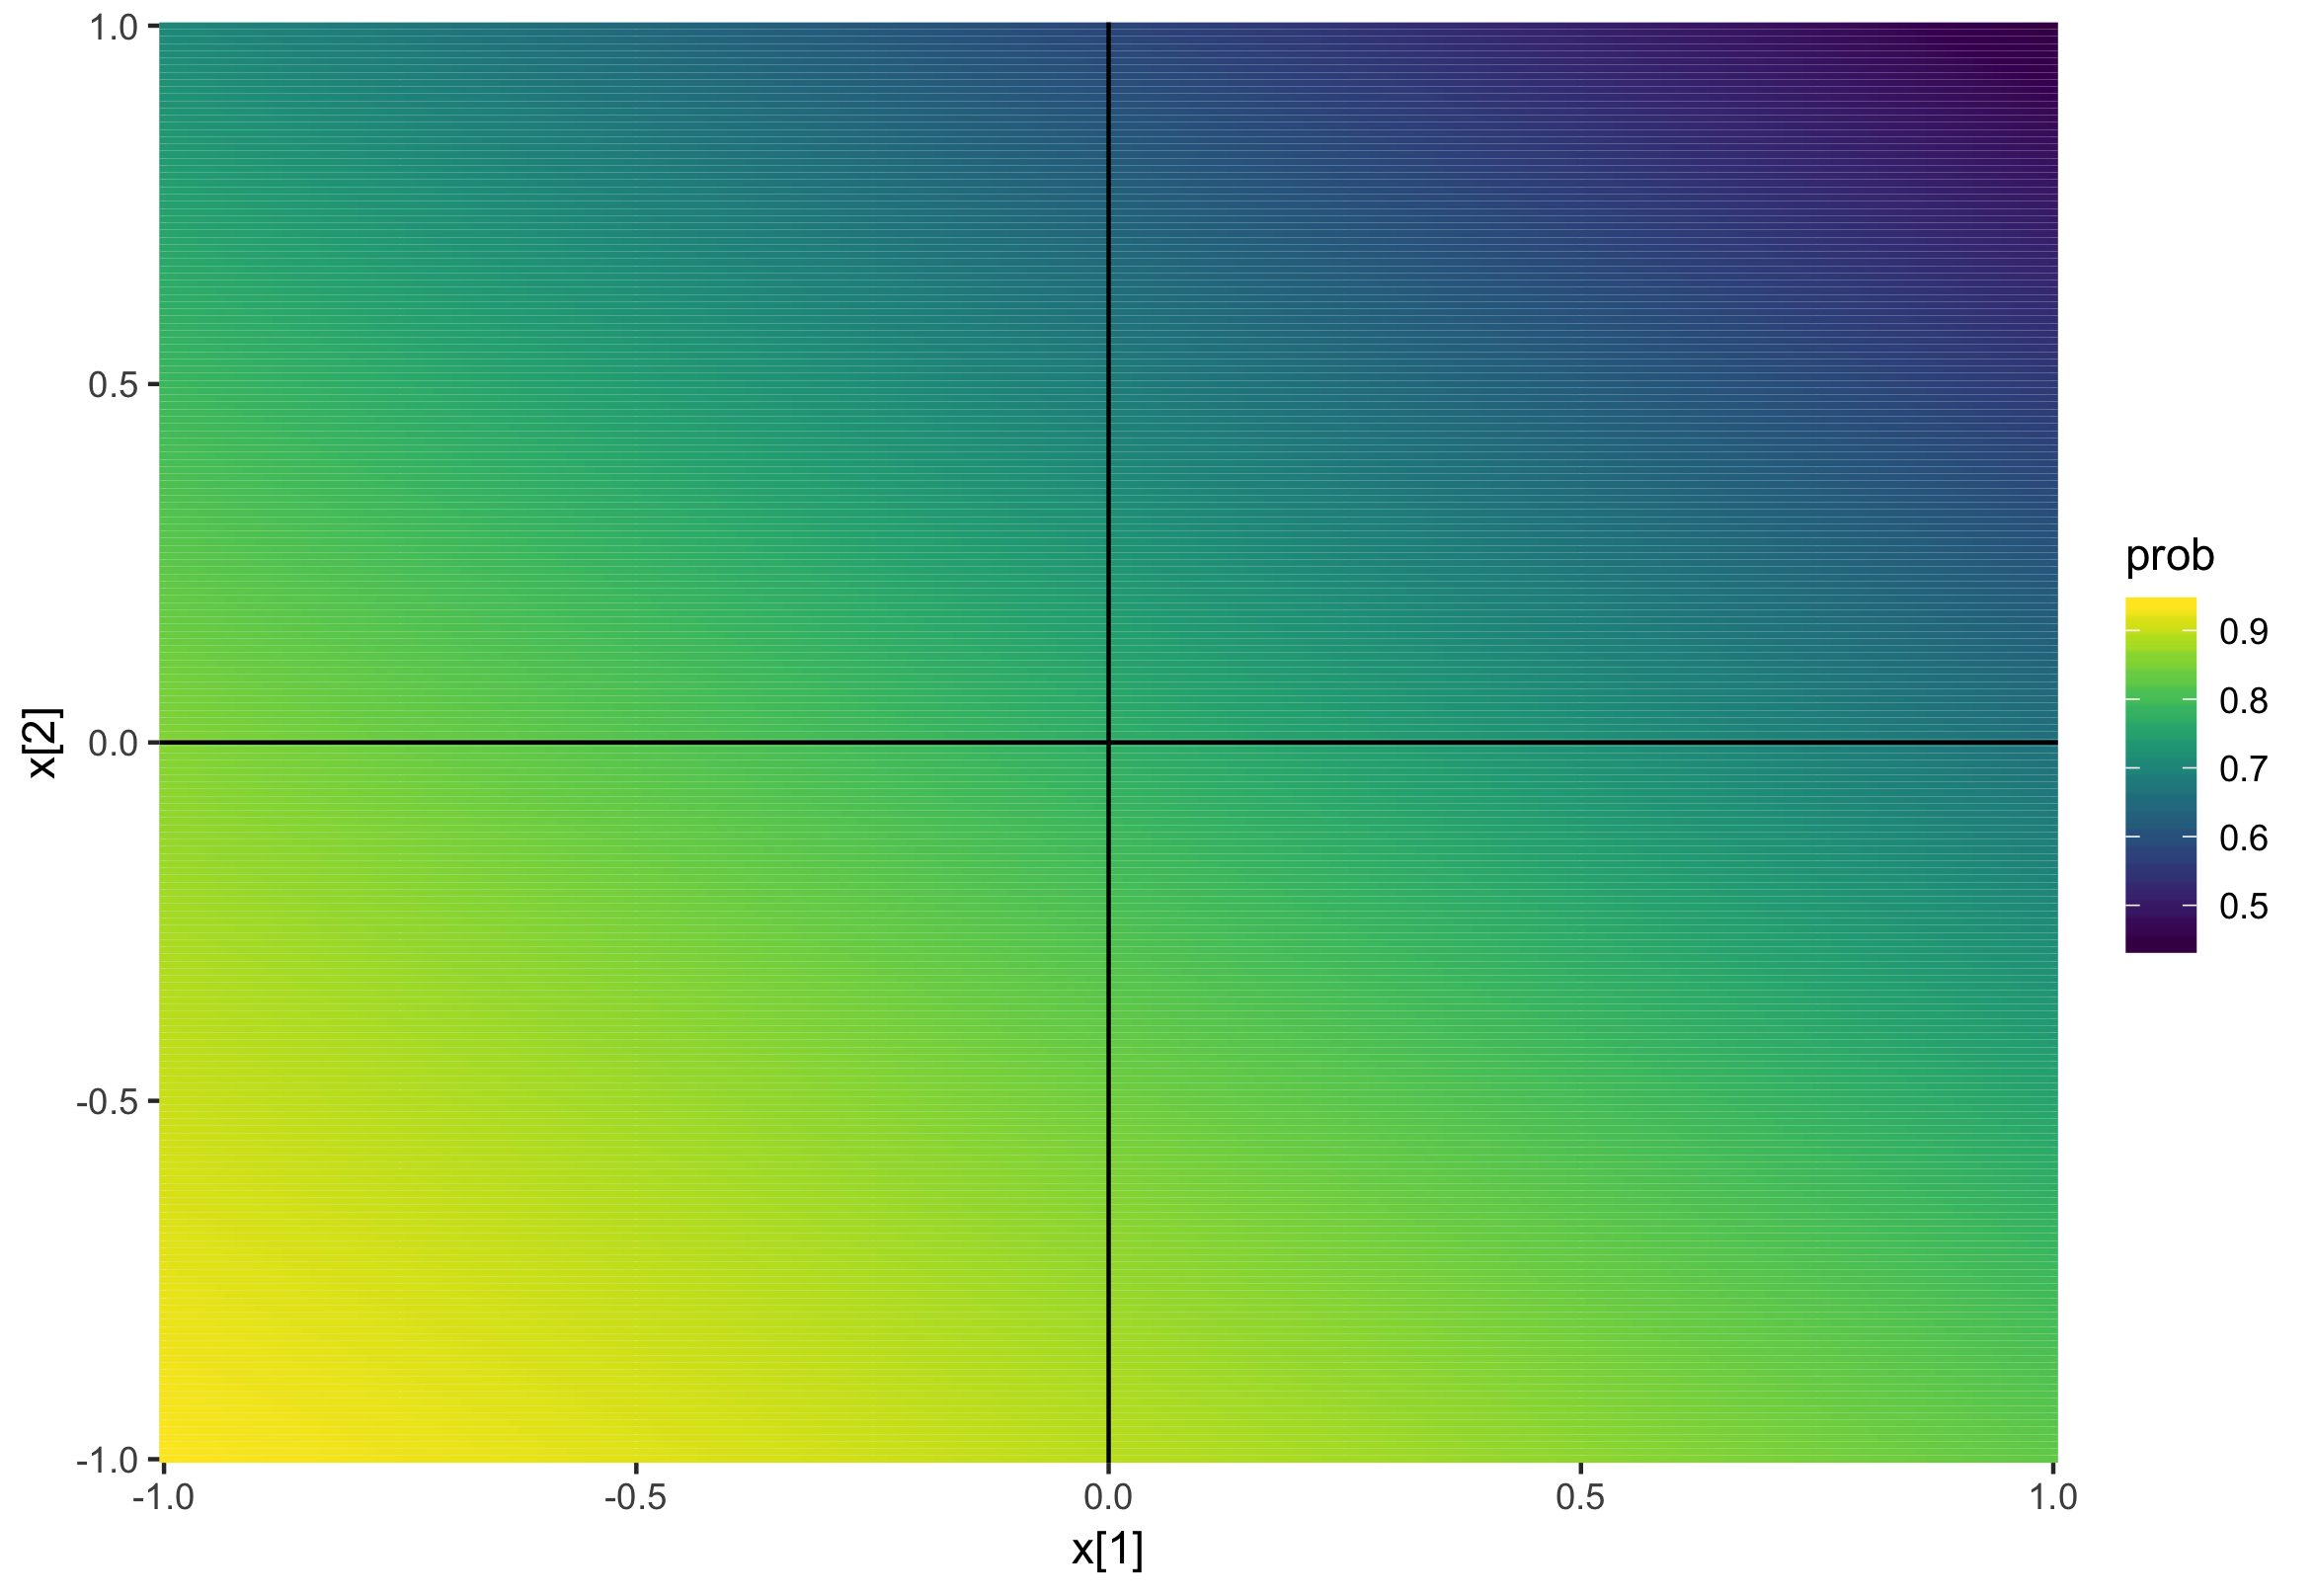
\includegraphics[width=0.17\paperwidth]{figure/sigmoid_plot_3}
    \end{subfigure}
    \begin{subfigure}{.17\paperwidth}
      \centering
      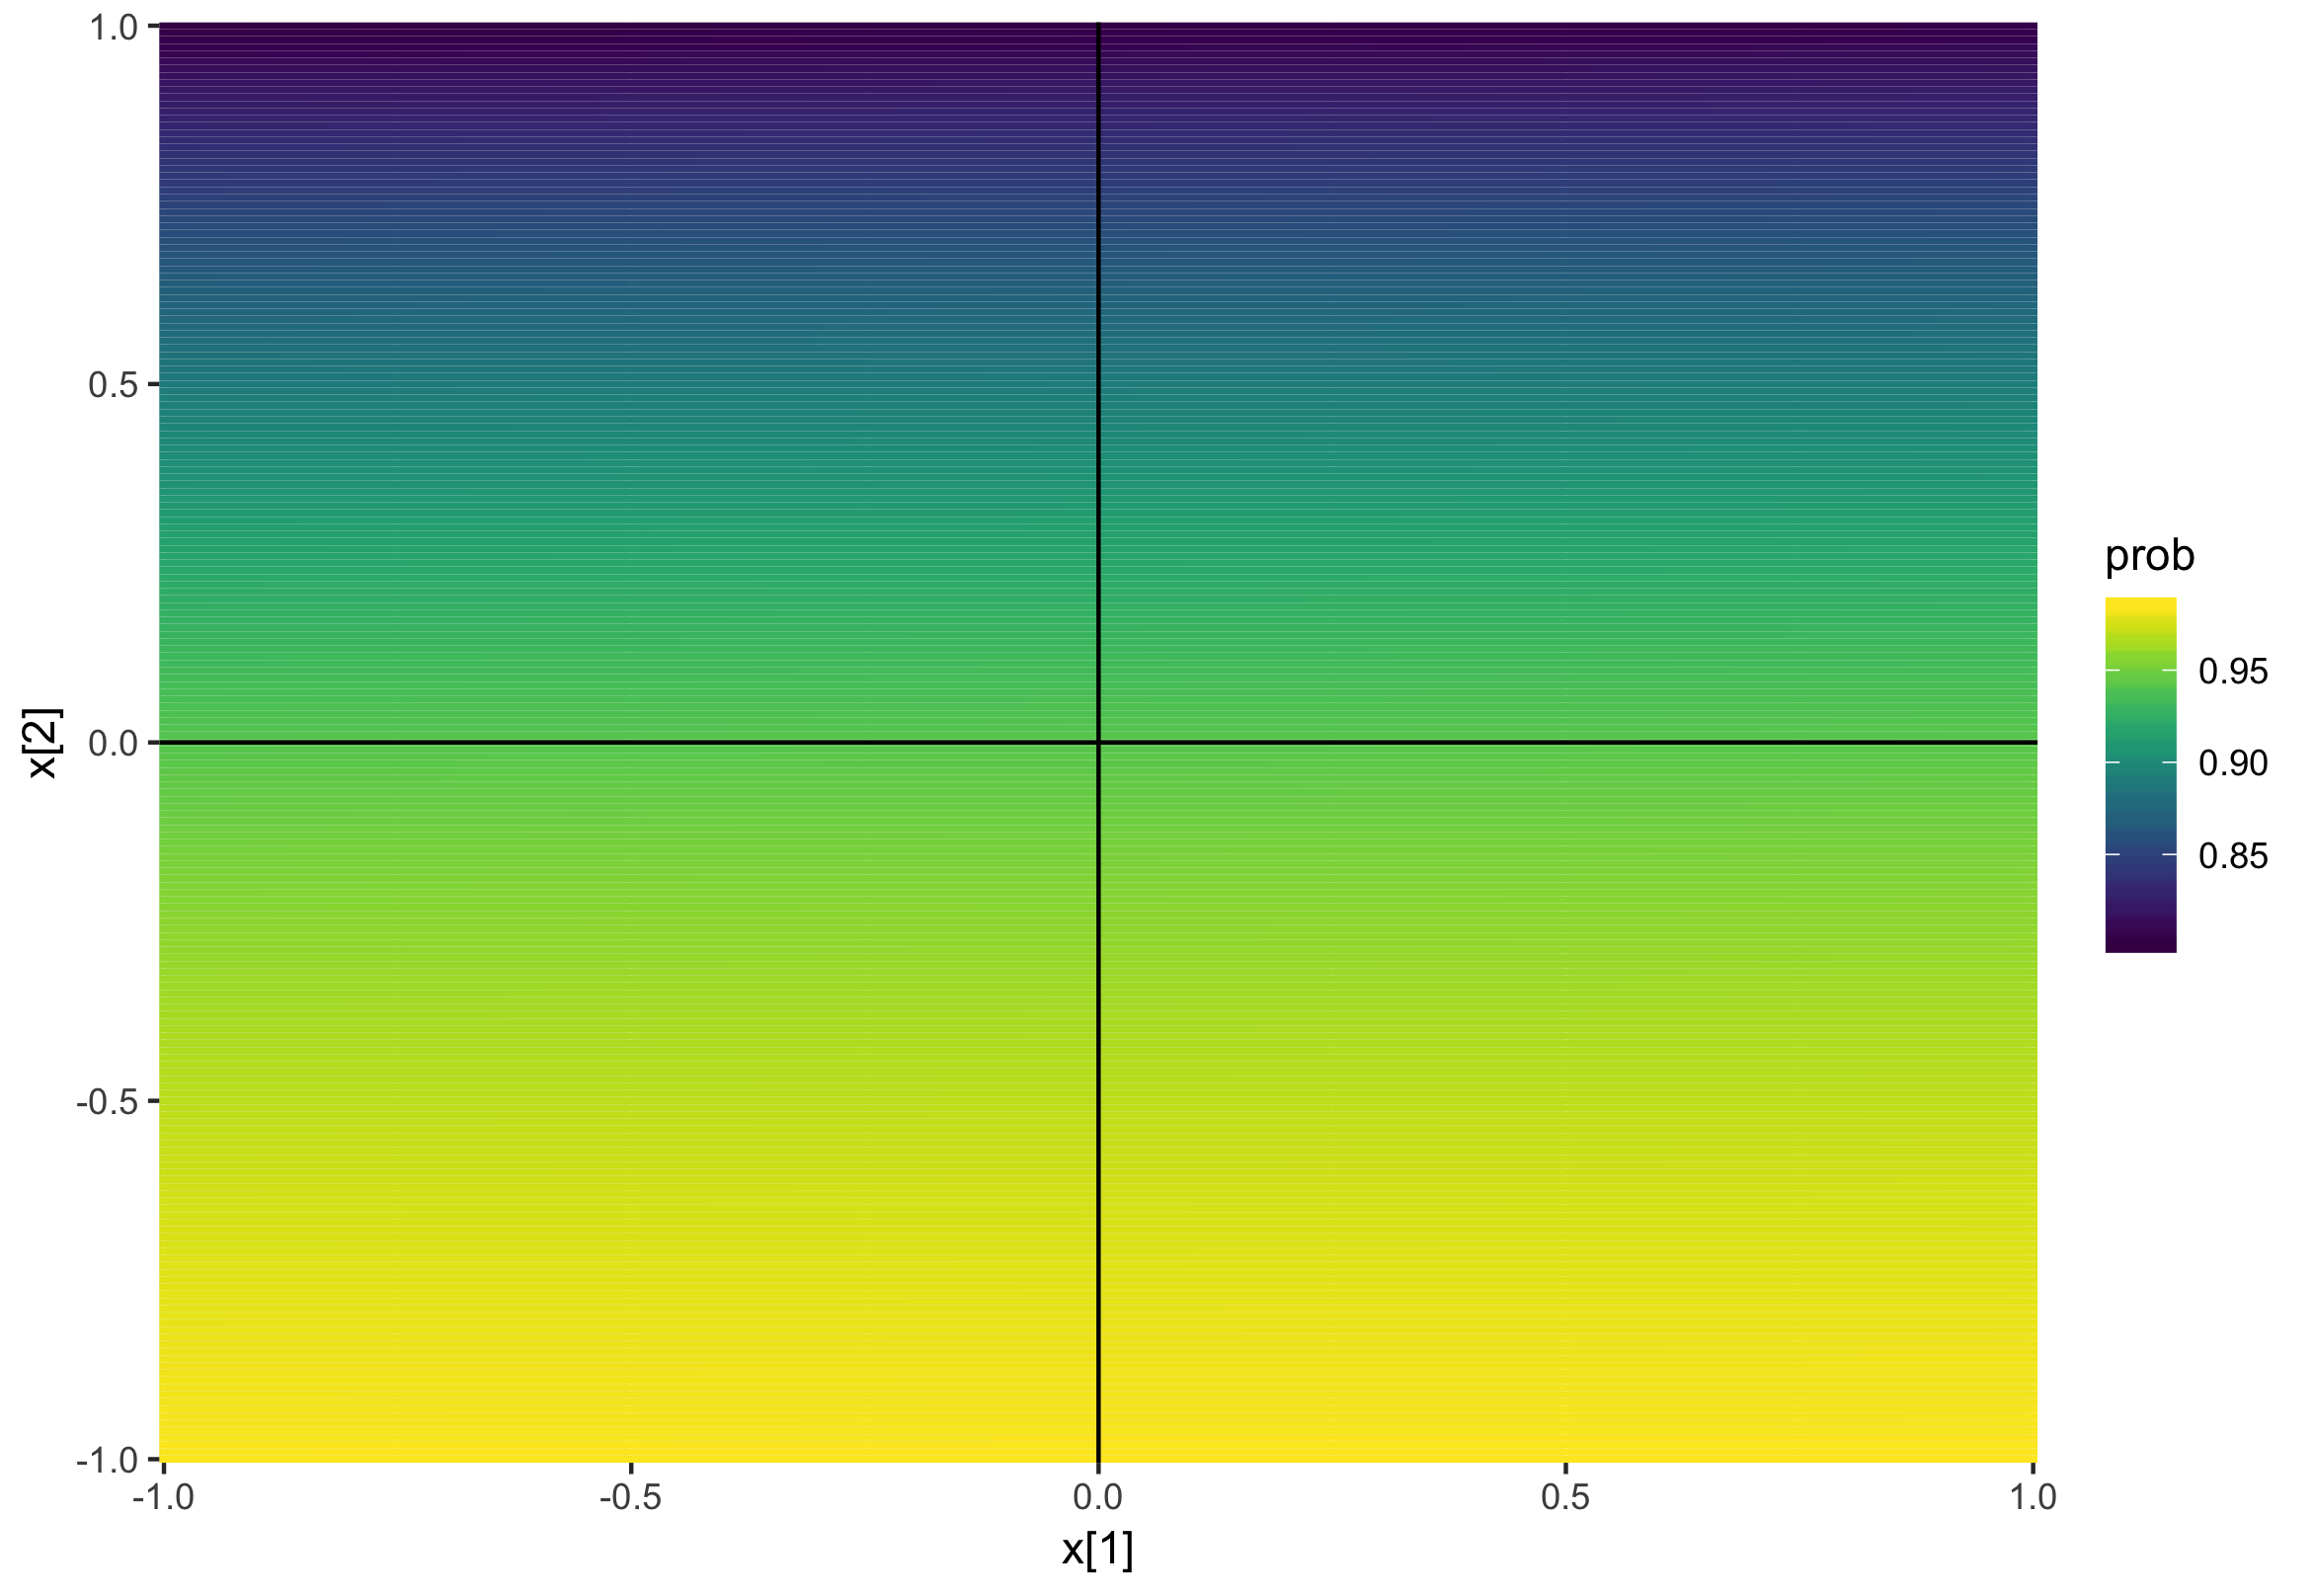
\includegraphics[width=0.17\paperwidth]{figure/sigmoid_plot_4}
    \end{subfigure}
    \begin{subfigure}{.17\paperwidth}
      \centering
      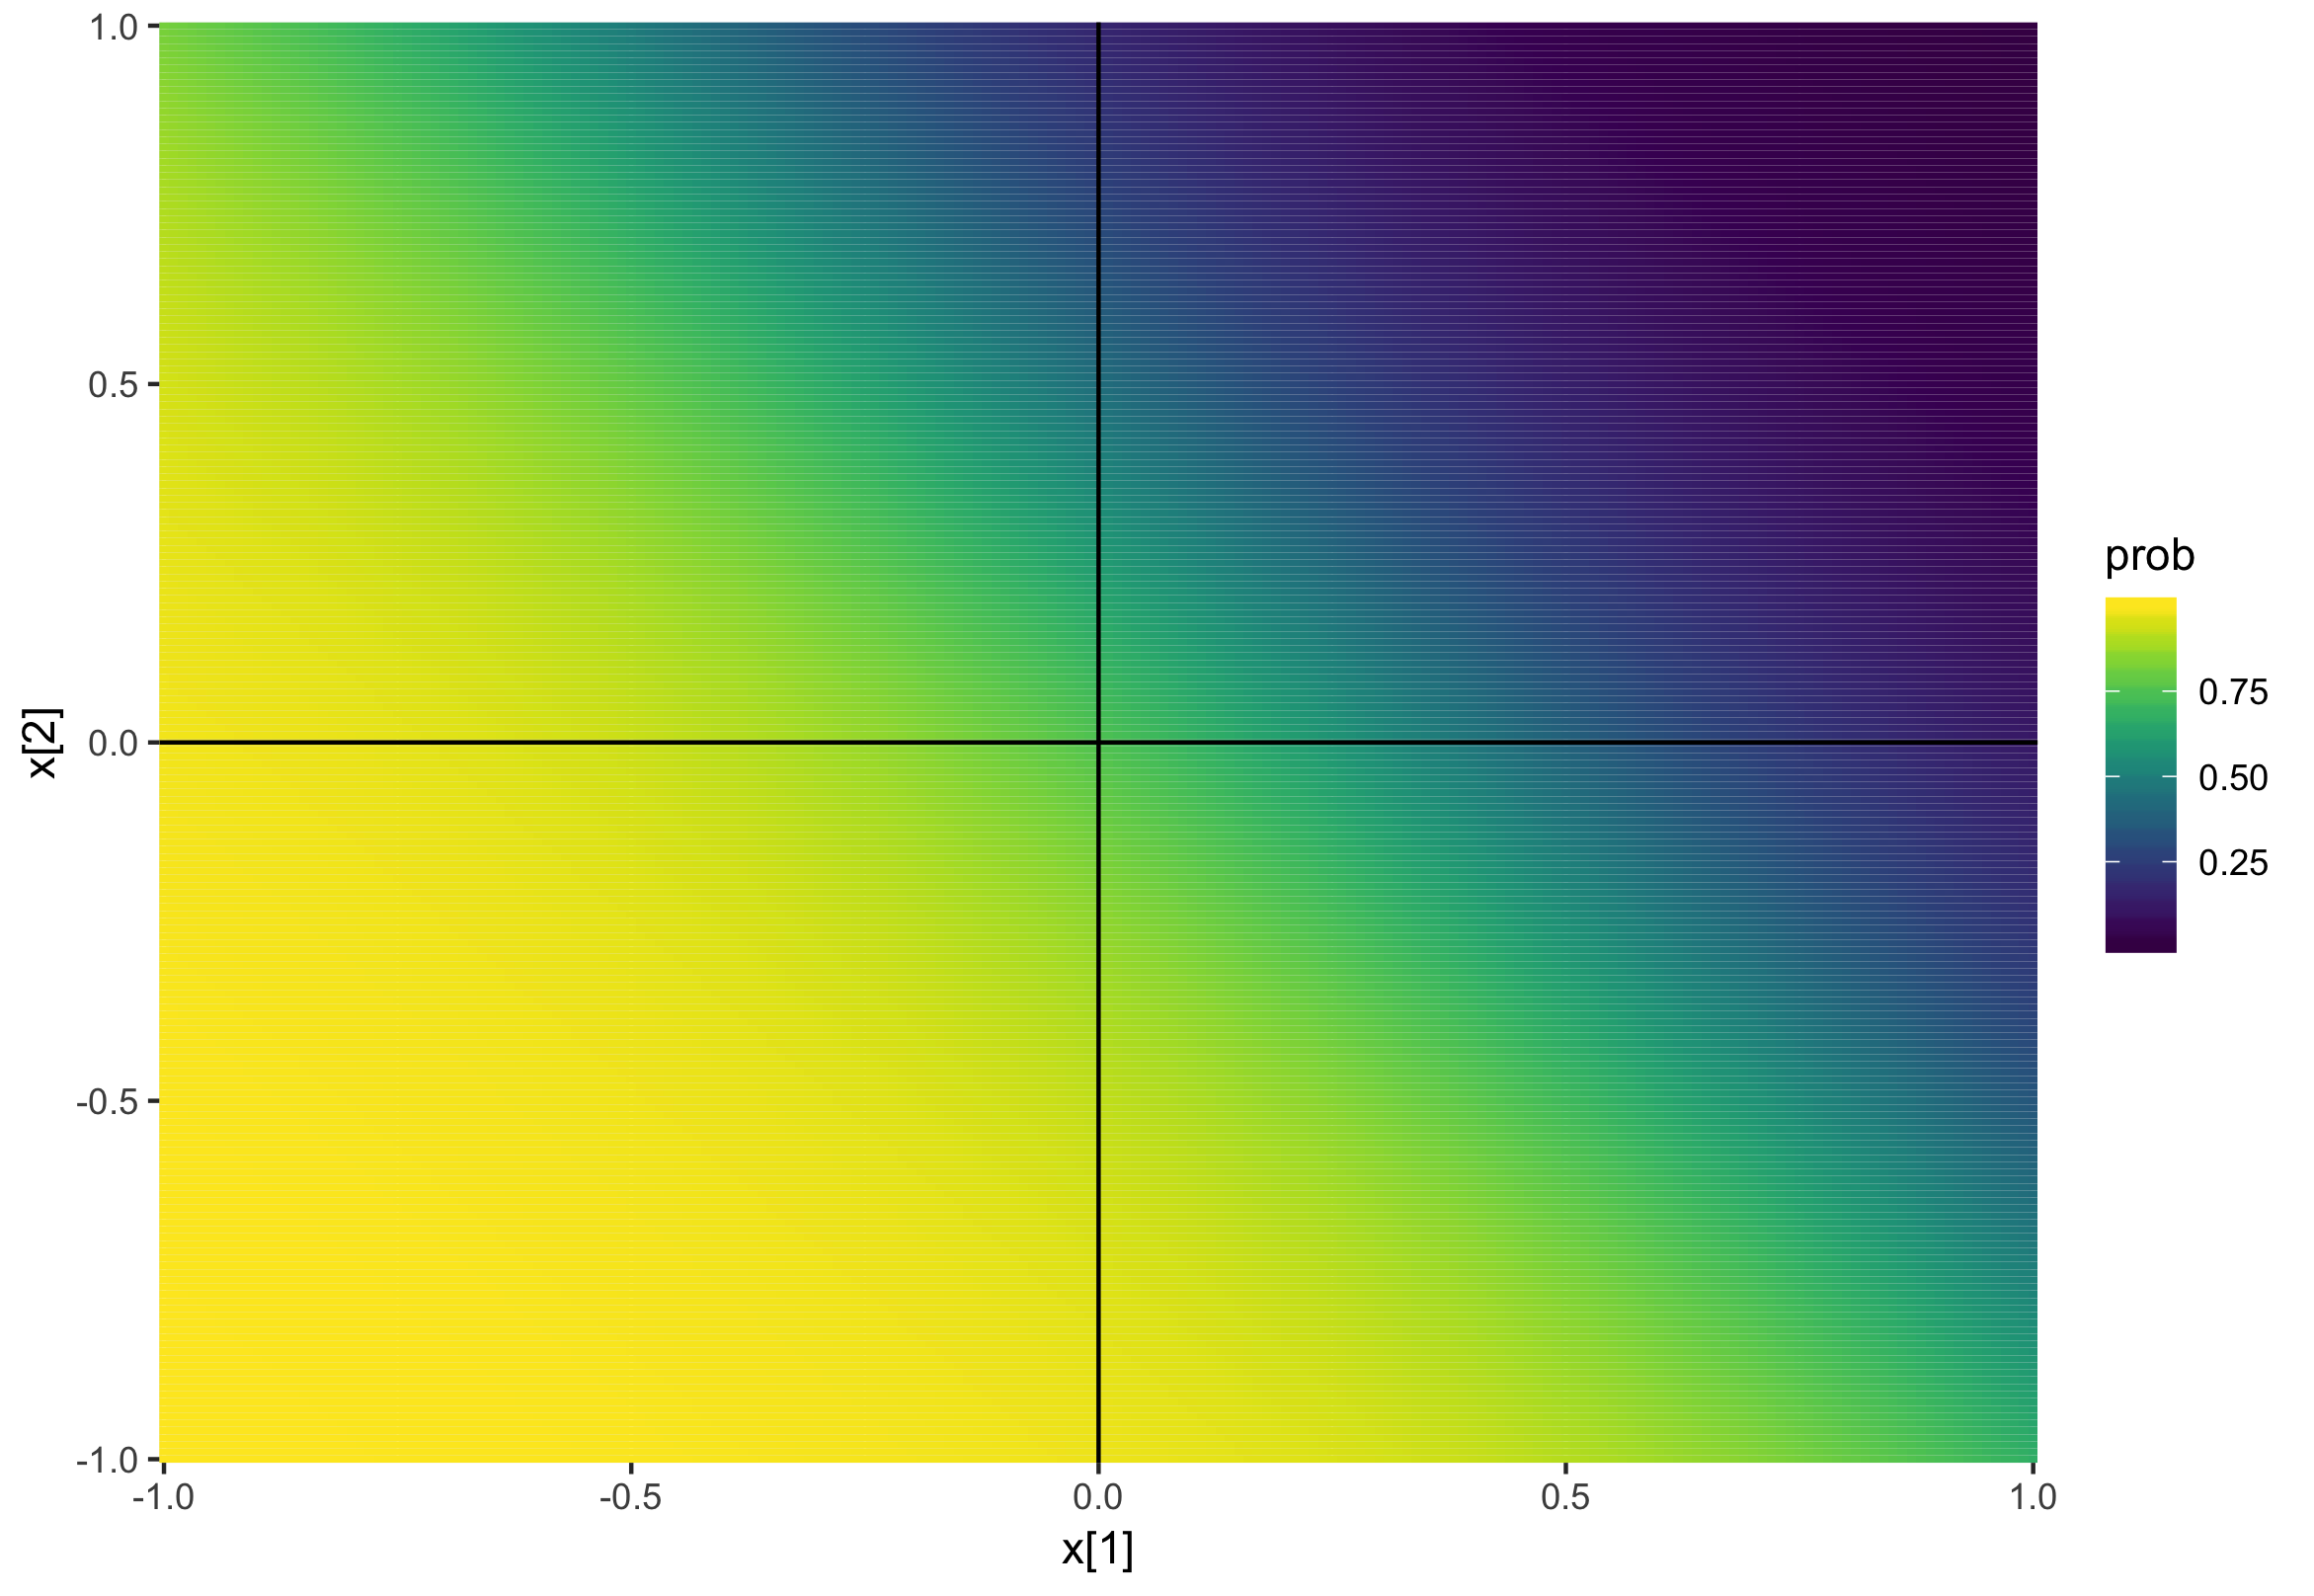
\includegraphics[width=0.17\paperwidth]{figure/sigmoid_plot_5}
    \end{subfigure}
    \begin{subfigure}{.17\paperwidth}
      \centering
      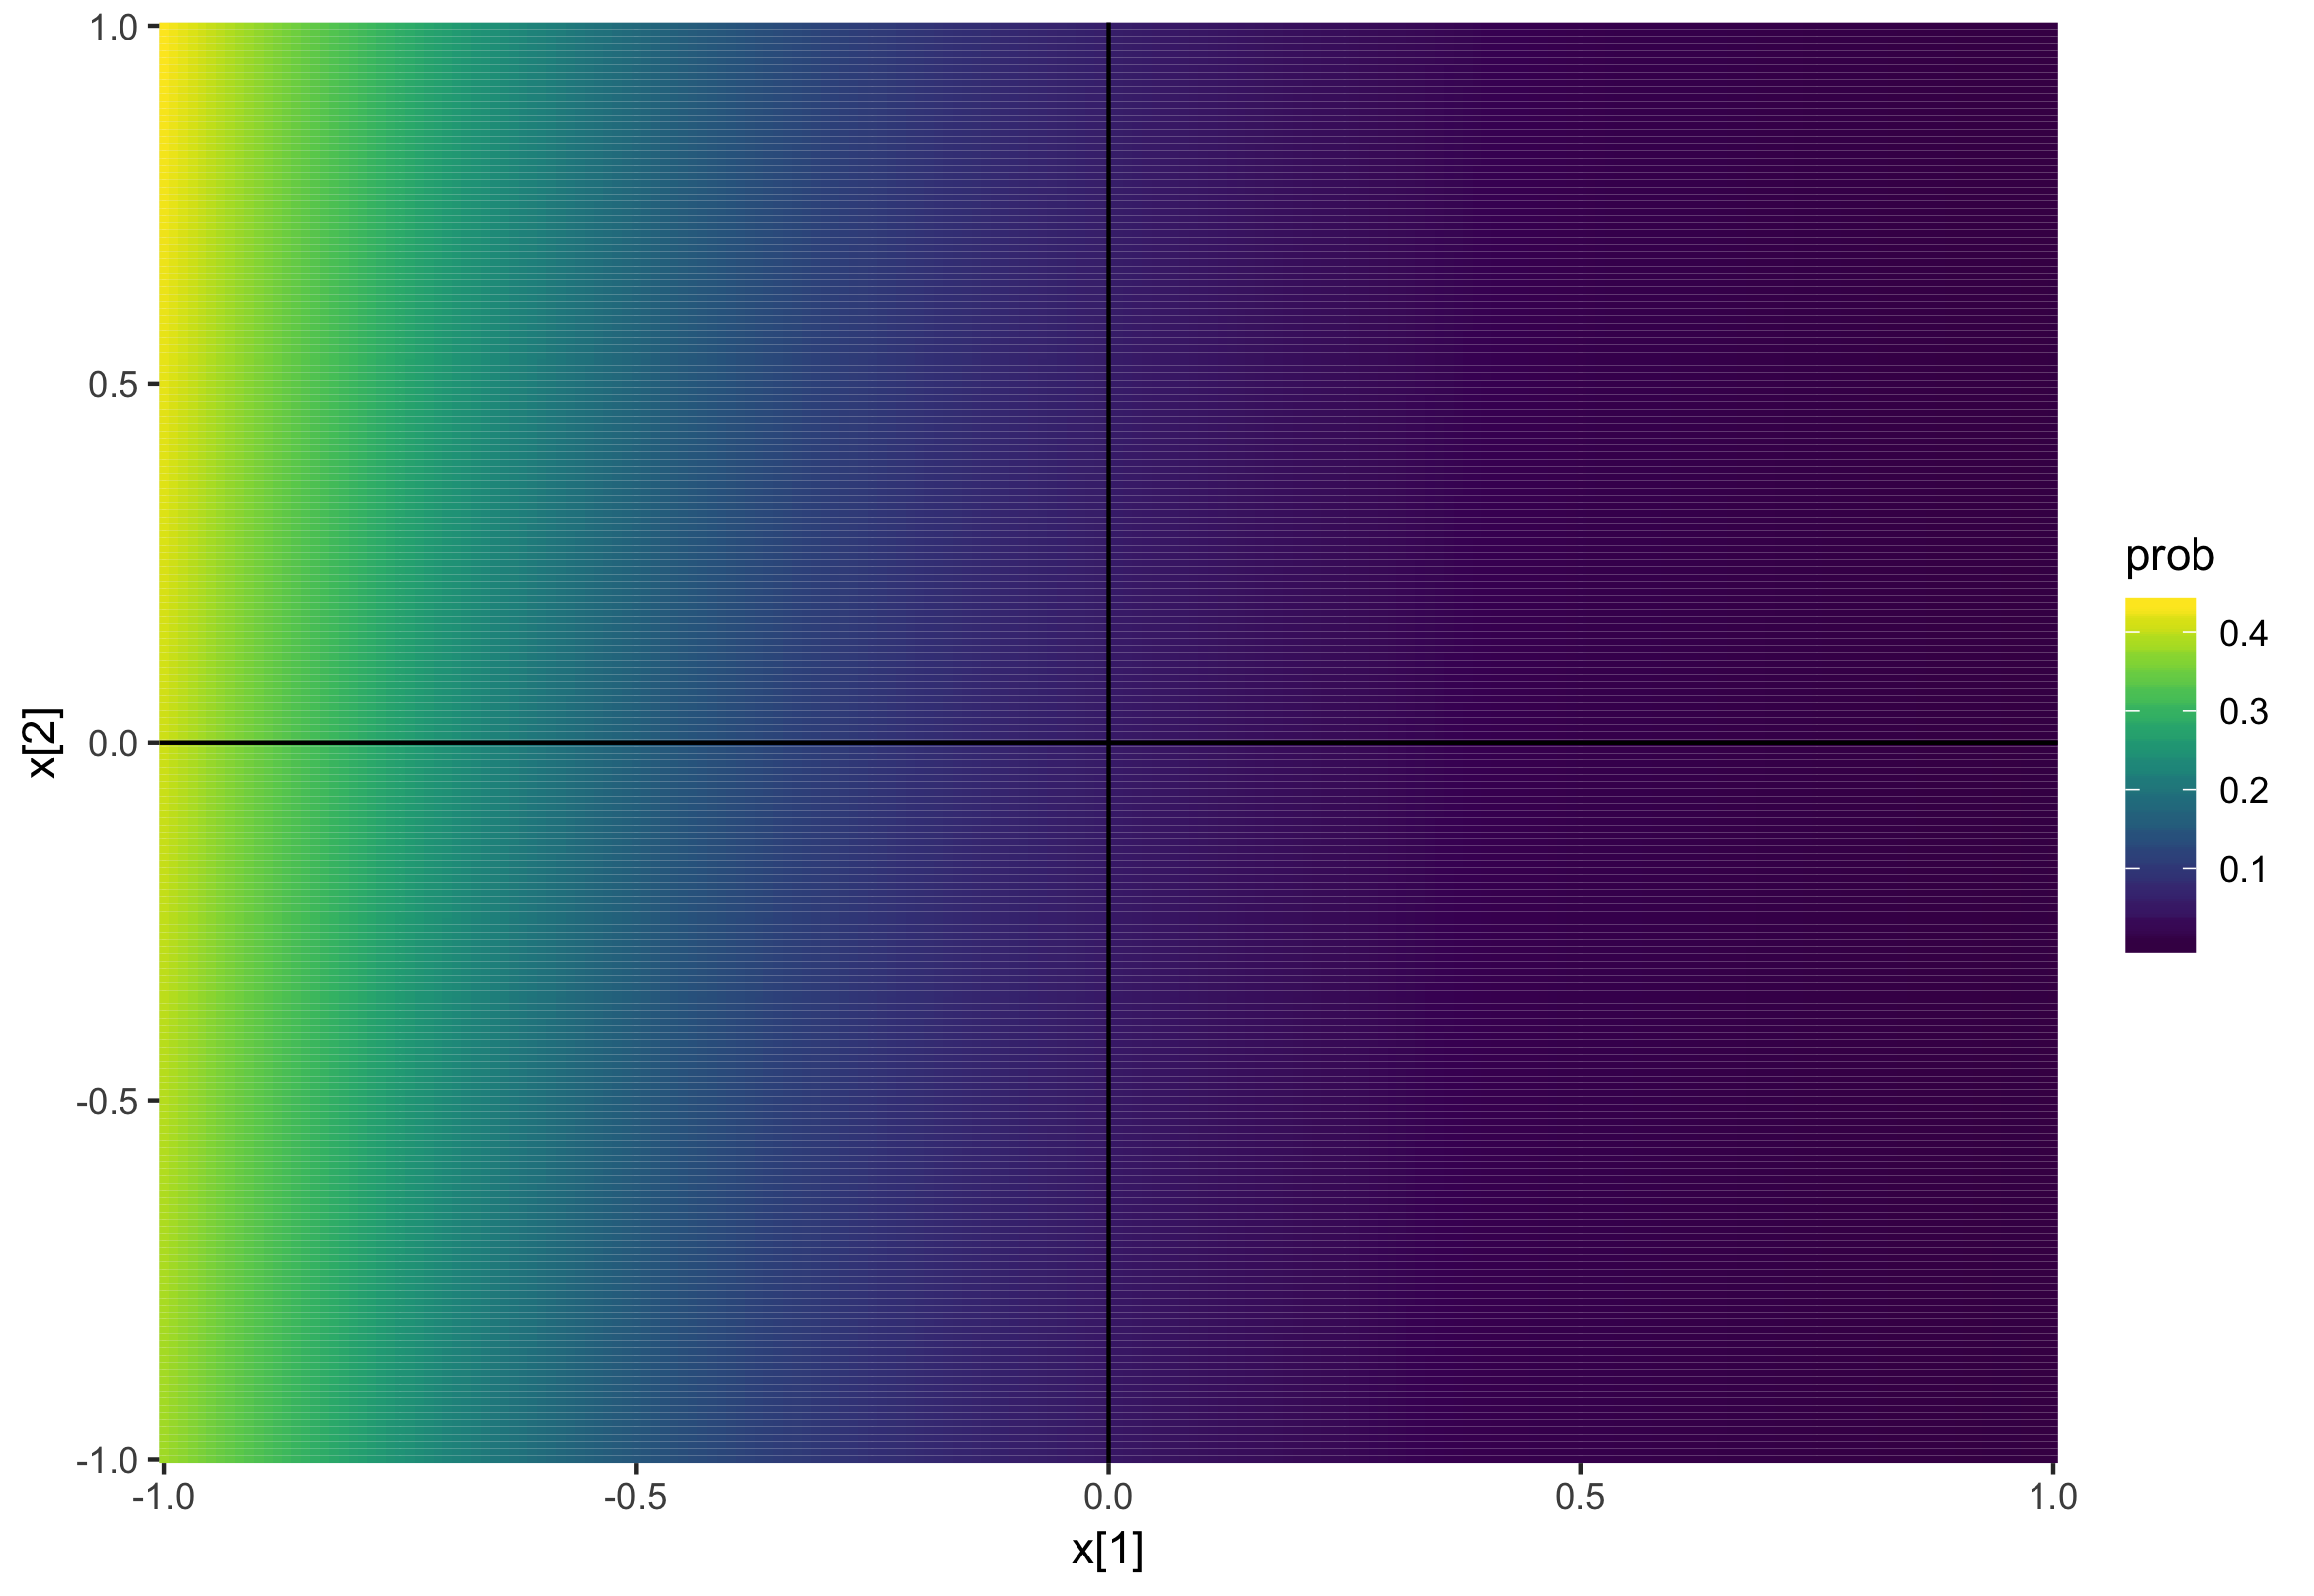
\includegraphics[width=0.17\paperwidth]{figure/sigmoid_plot_6}
    \end{subfigure}
    \begin{subfigure}{.17\paperwidth}
      \centering
      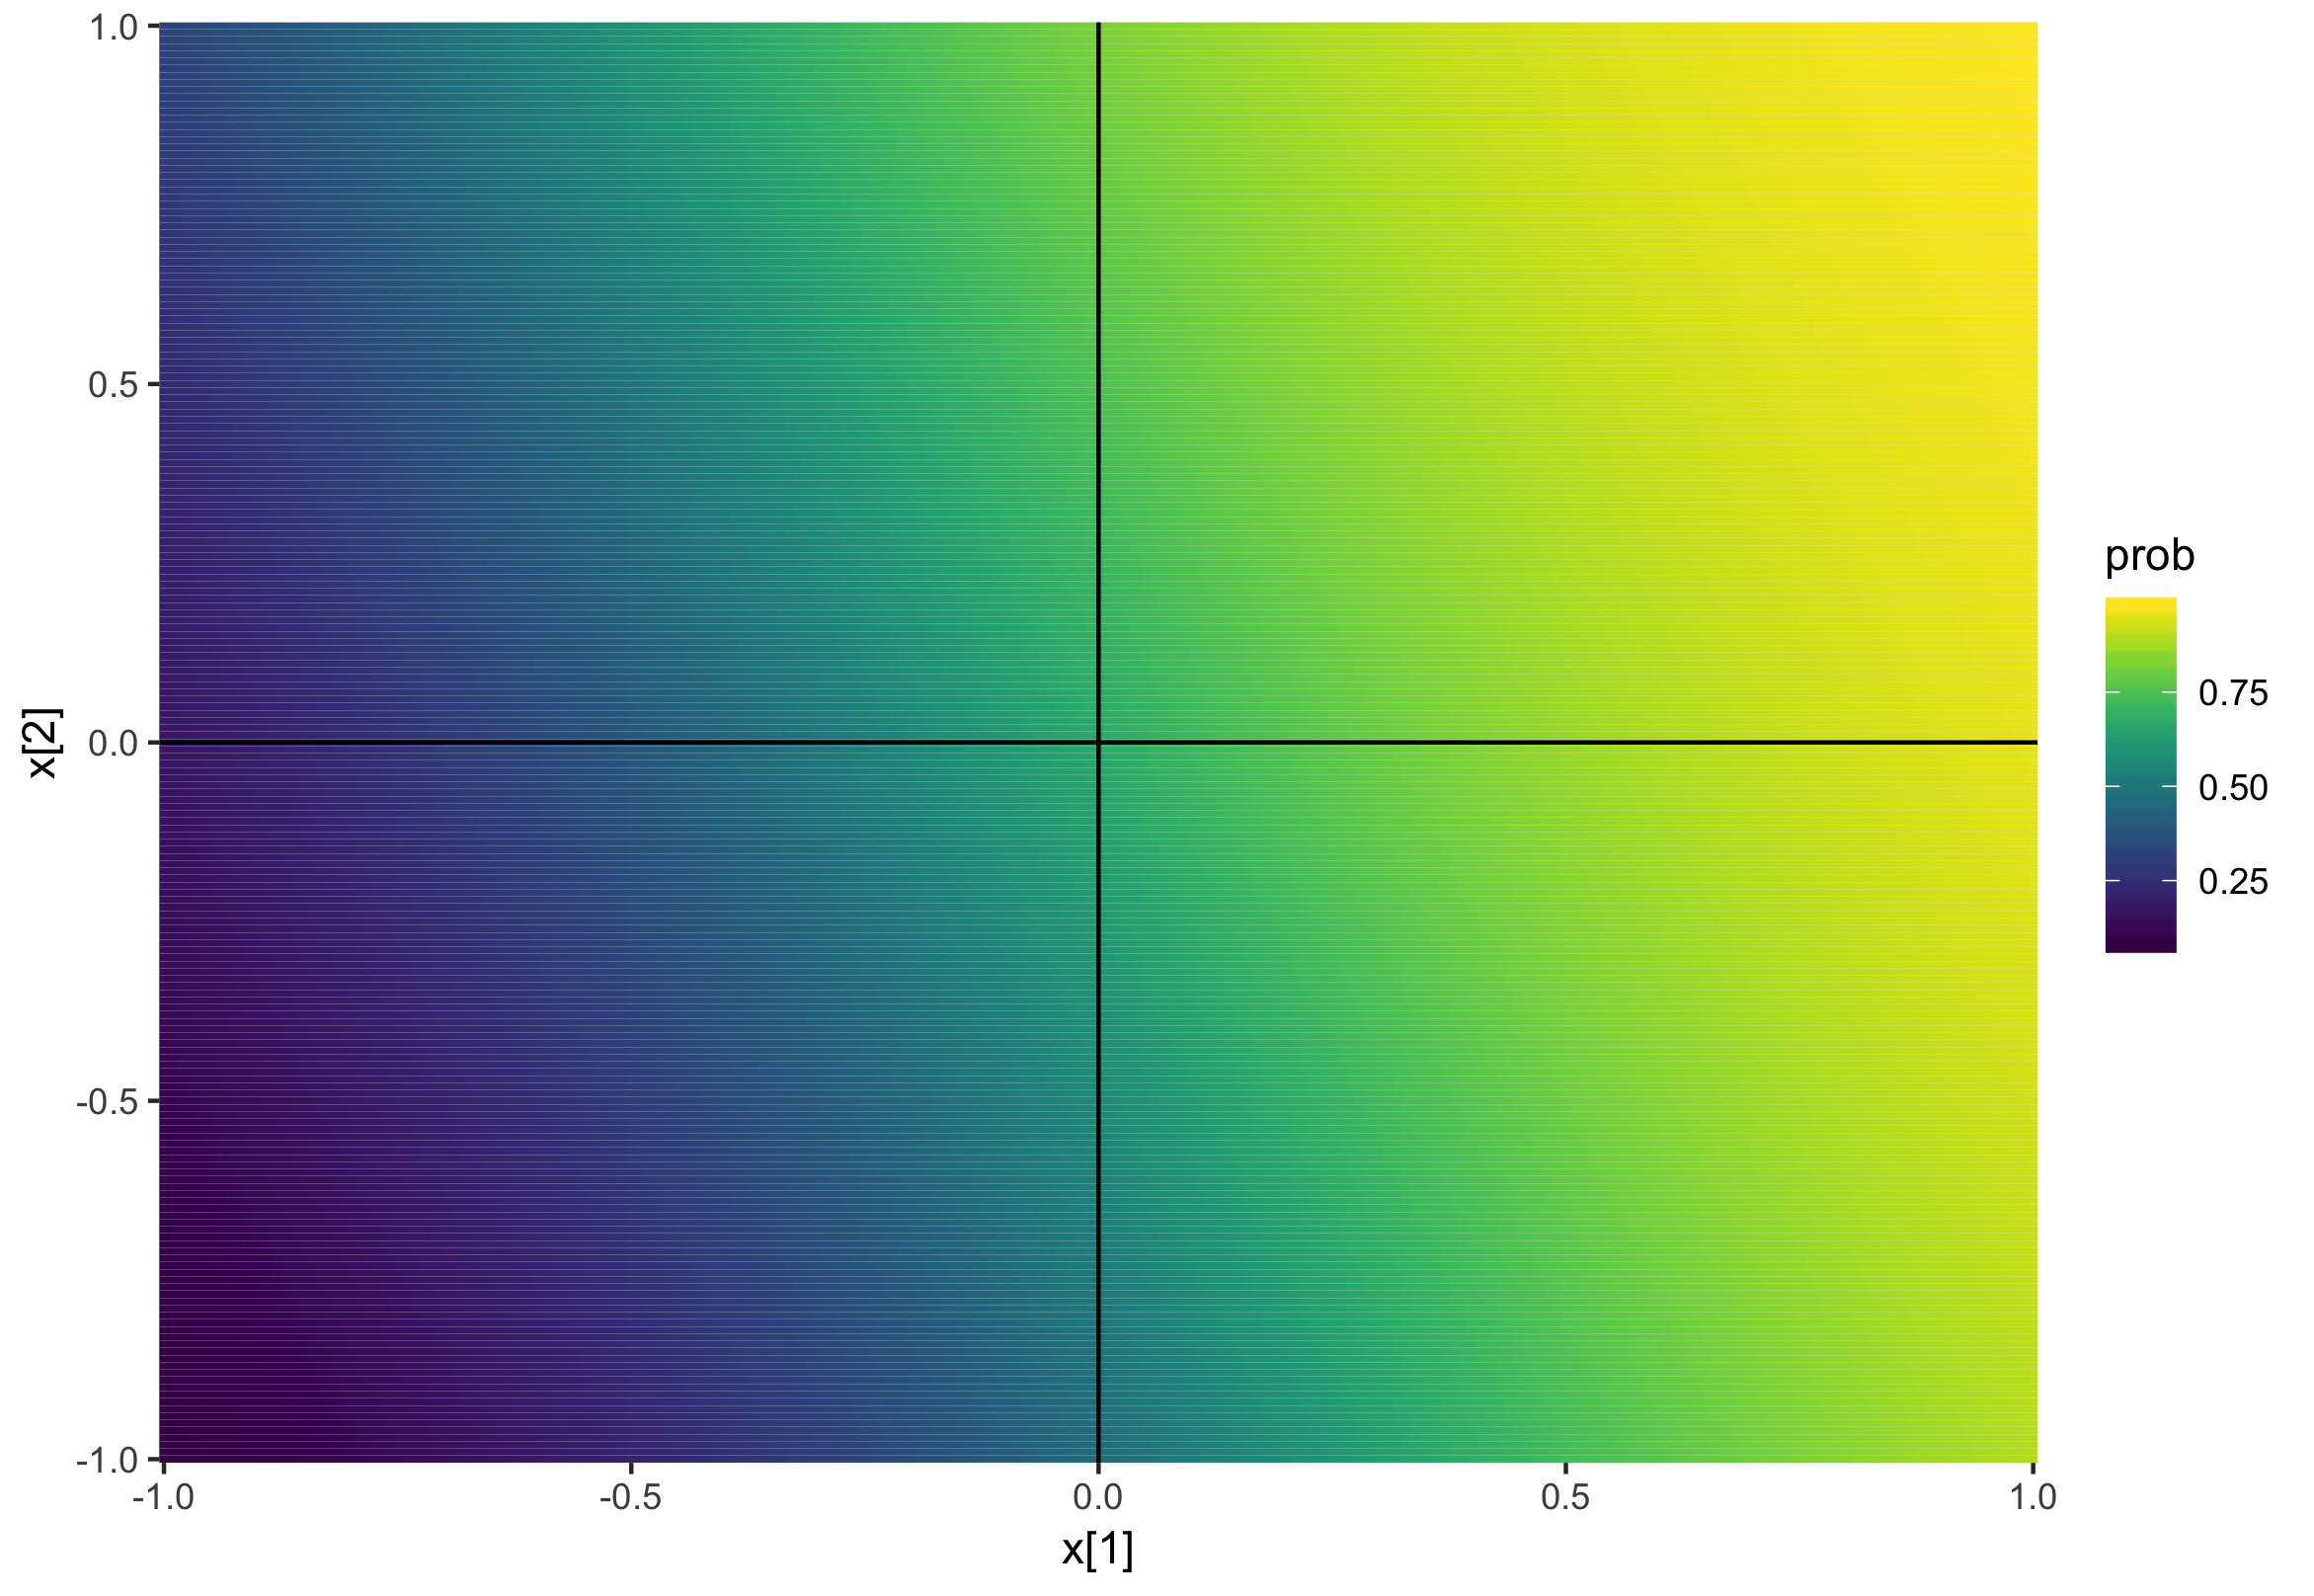
\includegraphics[width=0.17\paperwidth]{figure/sigmoid_plot_7}
    \end{subfigure}
    \begin{subfigure}{.17\paperwidth}
      \centering
      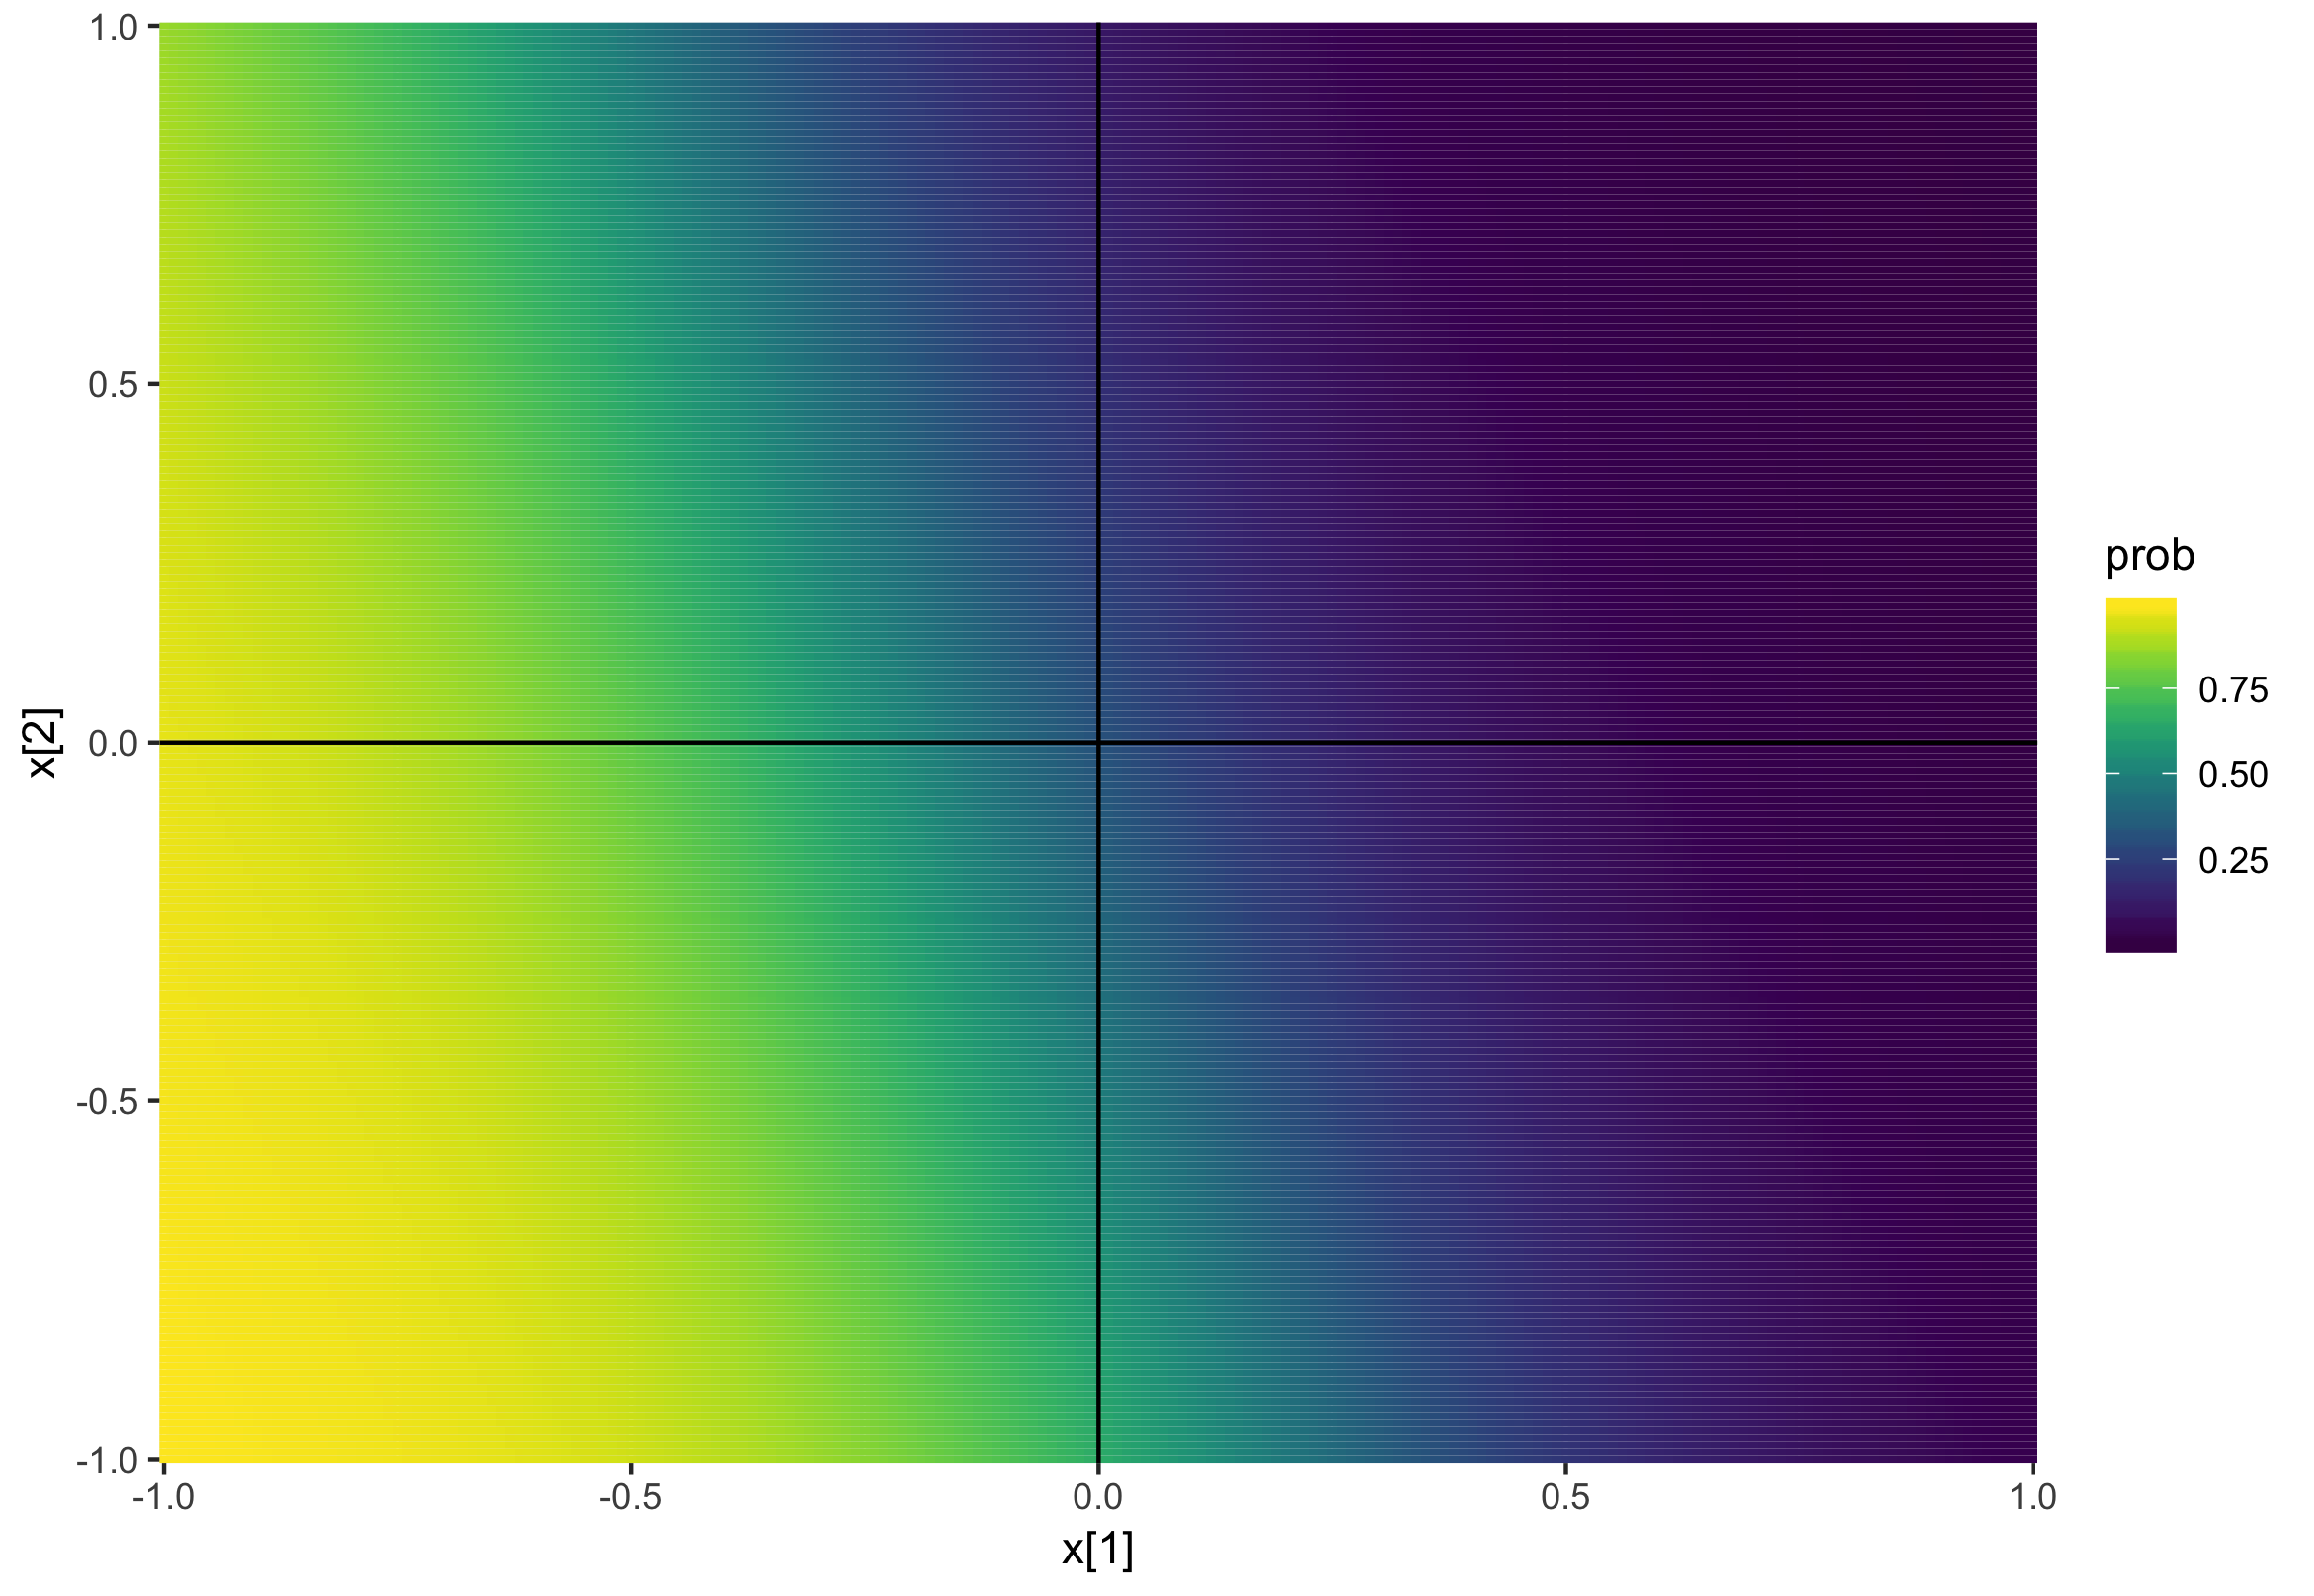
\includegraphics[width=0.17\paperwidth]{figure/sigmoid_plot_8}
    \end{subfigure}
    \begin{subfigure}{.17\paperwidth}
      \centering
      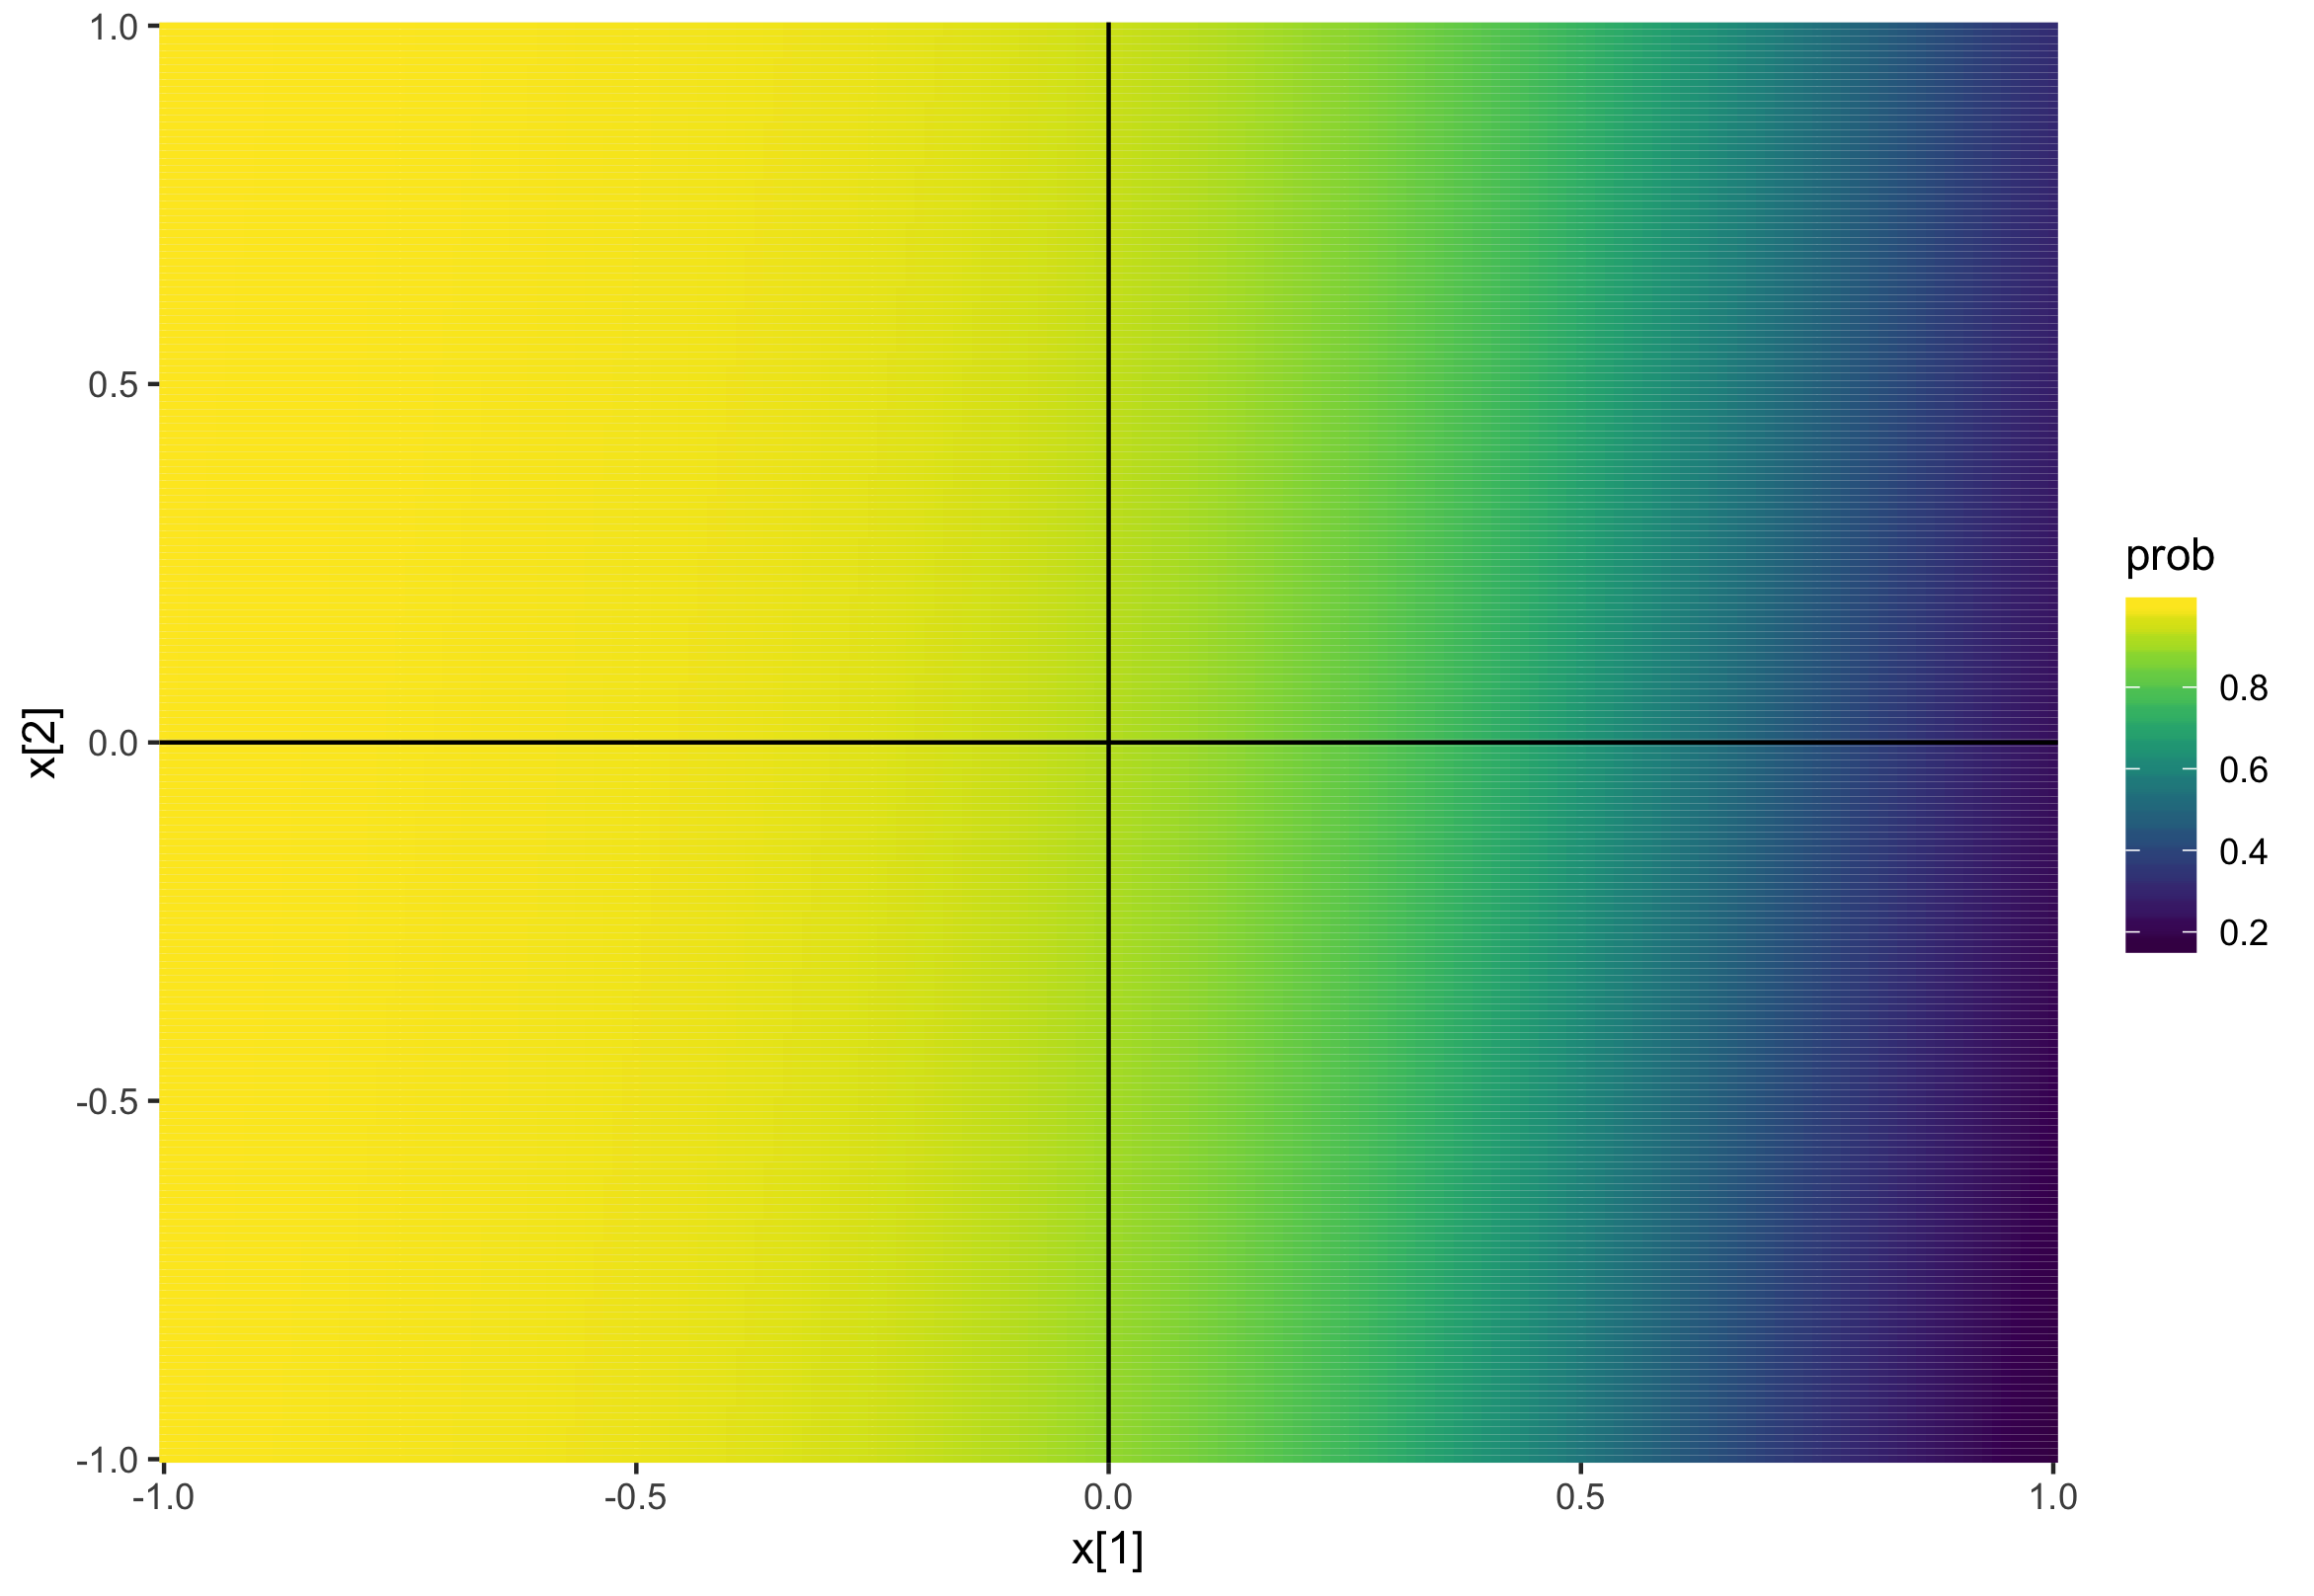
\includegraphics[width=0.17\paperwidth]{figure/sigmoid_plot_9}
    \end{subfigure}
    \begin{subfigure}{.17\paperwidth}
      \centering
      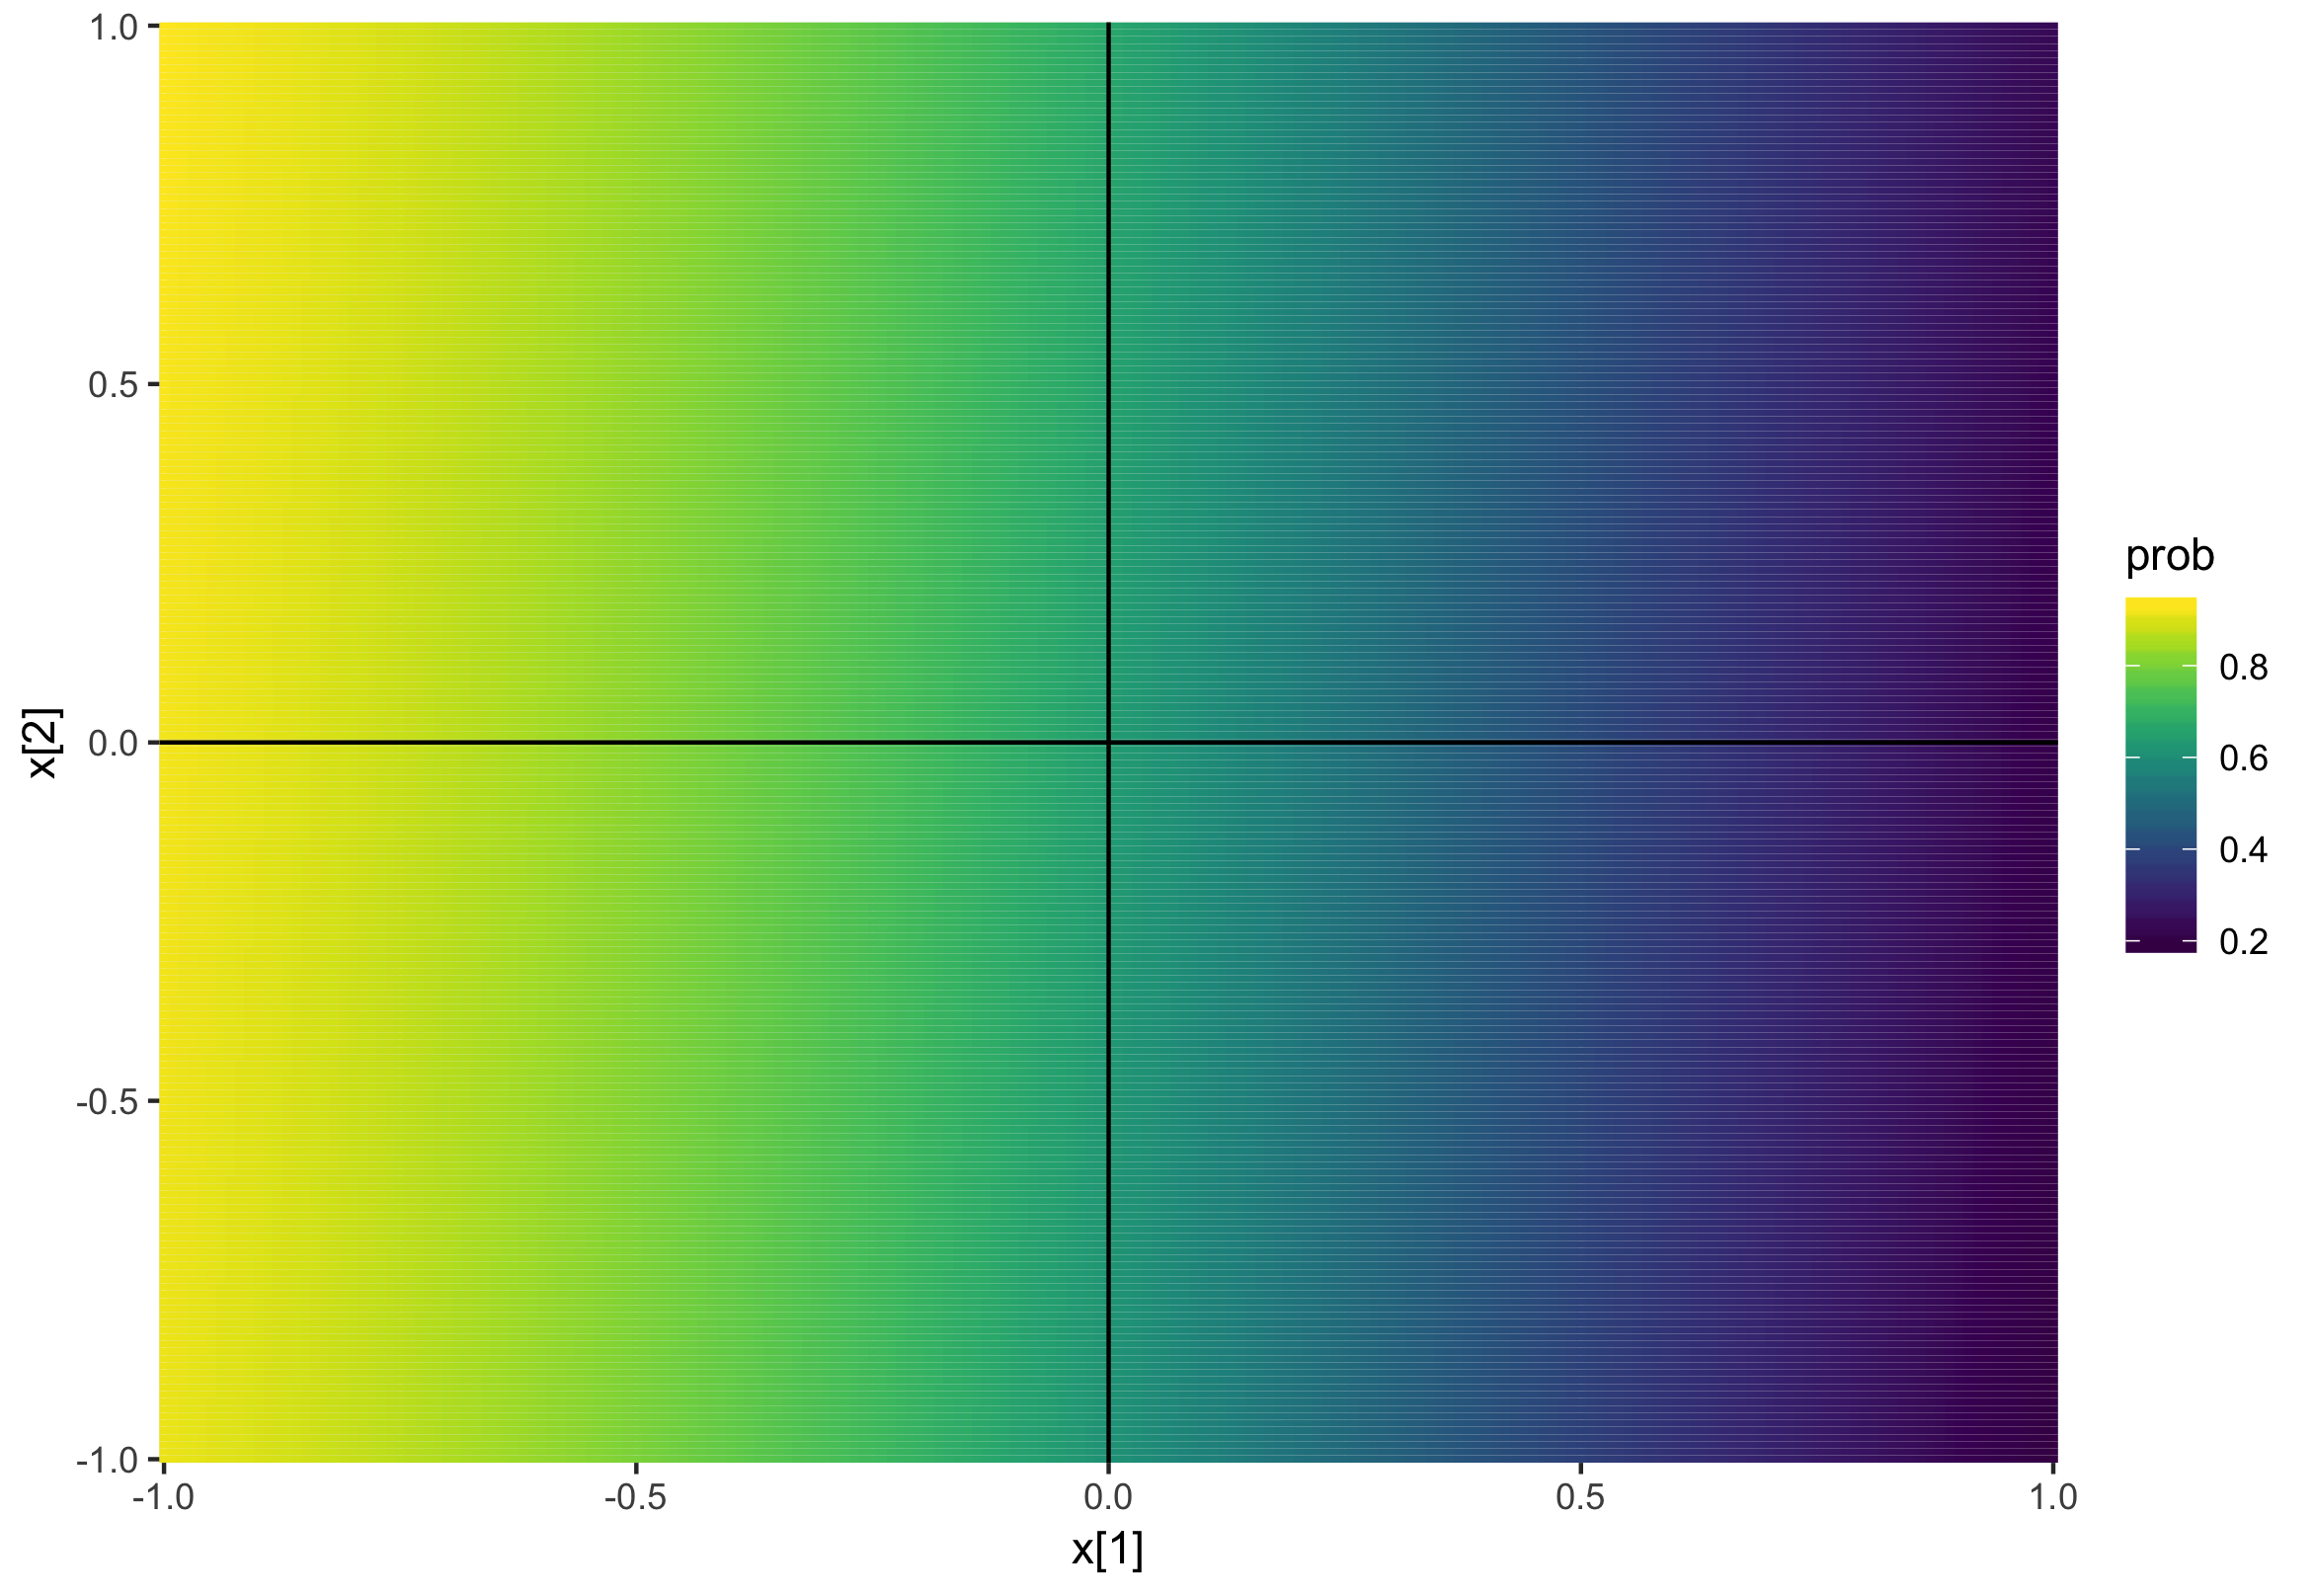
\includegraphics[width=0.17\paperwidth]{figure/sigmoid_plot_10}
    \end{subfigure}
    \caption{Example sigmoid functions $\pi_{\theta}$ for random draws of
      $\theta$, when we assume $x$ has an intercept term. Notice that there are
      no nonlinear boundaries...
      \label{fig:logistic_scatter_nonlinear} }
  \end{figure}
\end{frame}

\begin{frame}
  \frametitle{Logistic Regression}
  \begin{itemize}
  \item Logistic Regression $\rightarrow$ Finding good $\theta$'s for this
    likelihood (i.e., the ones that maximize it)
    \begin{align*}
      \log p_{\theta}\left(y \vert x\right) &= \sum_{i = 1}^{n} \indic{y_i = 1}\log \pi_{\theta}\left(x\right) + \indic{y_i = 0}\log\left(1 - \pi_{\theta}\left(x\right)\right)
    \end{align*}
  \item These are the directions like those in the previous figure that do a
    good job separating heads from tails
  \end{itemize}
\end{frame}

\begin{frame}
  \frametitle{Optimization}
  \begin{itemize}
  \item Need to find some $\theta$'s that maximize $\log p_{\theta}\left(y \vert s\right)$
  \item Use gradient descent on $-\log p_{\theta}\left(y \vert x\right)$
  \item How to get the gradients?
  \item Approach 1: Courageously differentiate,
    \begin{align*}
      &\frac{\partial}{\partial \theta}\log p_{\theta}\left(y \vert x\right) \\
      = &\frac{\partial}{\partial \theta} \left[\sum_{i = 1}^{n} y_i \log \sigma\left(\theta^{T}x_{i}\right) + \left(1 - y_i\right)\log\left(1 - \sigma\left(\theta^{T}x_i\right)\right)\right] \\
      = &\frac{\partial}{\partial \theta}\left[\sum_{i = 1}^{n}
        y_i \log\left(\frac{1}{1 + \exp{-\theta^{T}x_i}}\right) +
          \left(1 - y_i\right)\log\left(\frac{\exp{-\theta^{T}x_i}}{1 + \exp{-\theta^{T}x_i}}\right) \right]
    \end{align*}
  \end{itemize}
\end{frame}

\begin{frame}
  \frametitle{Optimization}
  \begin{itemize}
  \item Approach 2: Chain rule magic!
    \begin{align*}
      \log p_{\theta}\left(y_i \vert x_i\right)  &= y_i \log\left(\theta^T x_i\right) + \left(1 - y_i\right) \log\left(1 - \sigma\left(\theta^T x_i\right)\right) \\
      &= \ell\left(\sigma\left(\theta^T x_{i}\right)\right)
    \end{align*}
  \item This is the composition of three relatively simple functions
  \end{itemize}
\begin{figure}[ht]
  \centering
  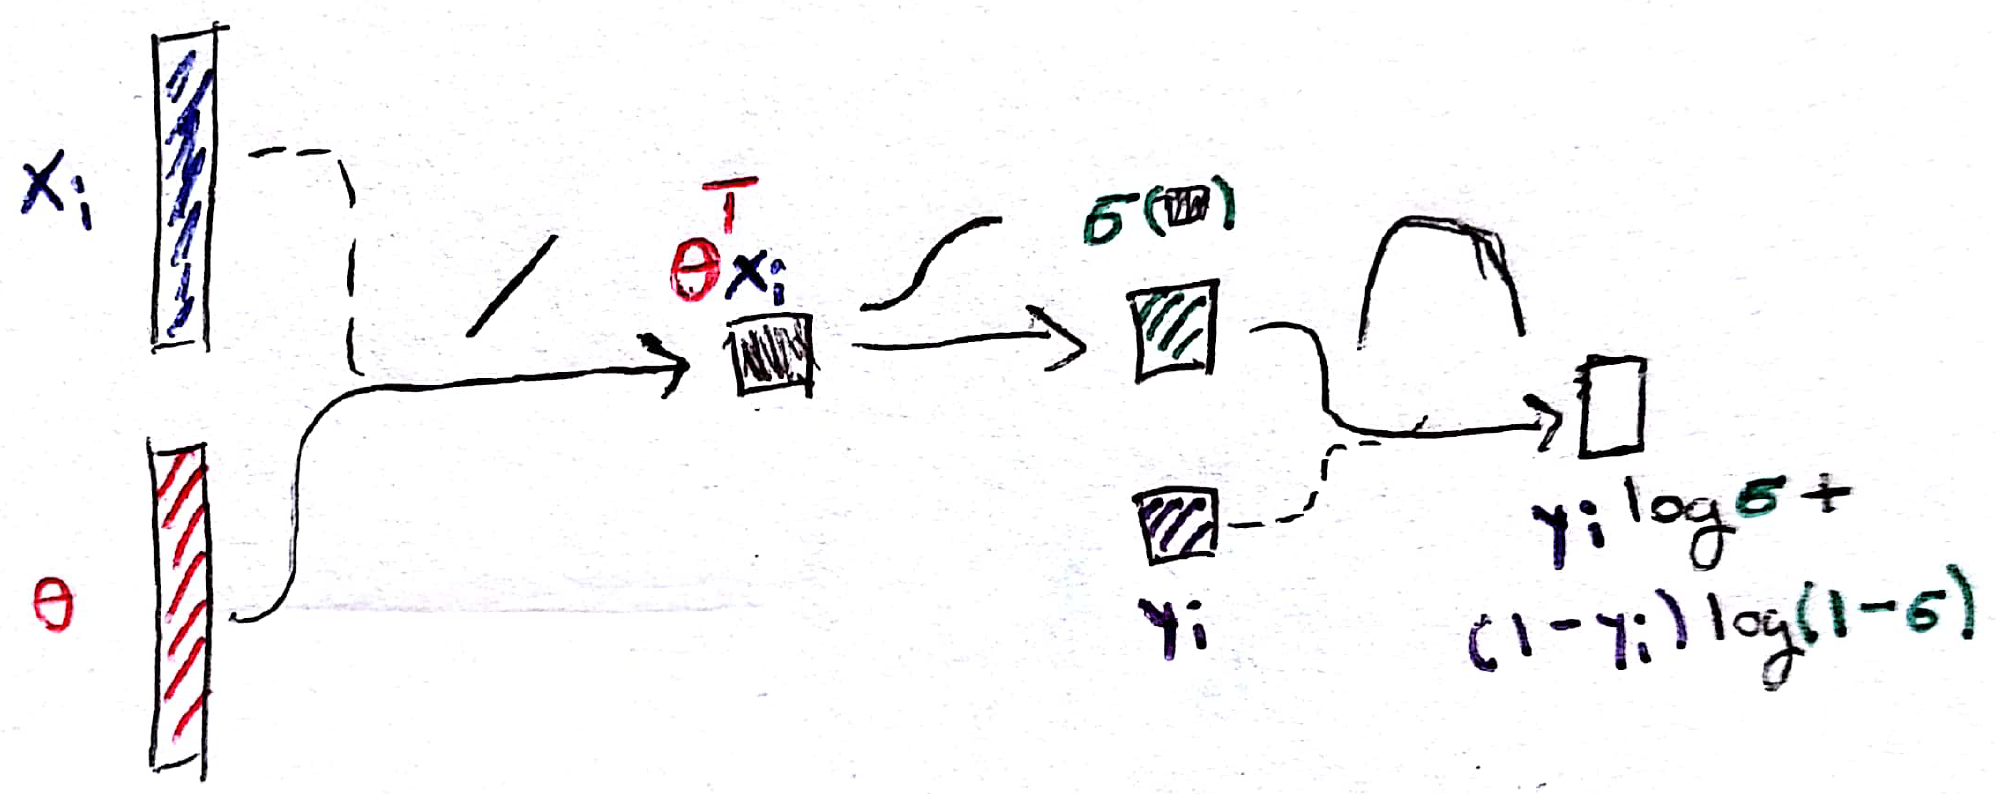
\includegraphics[width=0.7\paperwidth]{figure/logistic_comp_graph}
  \caption{The loss function is a series of compositions of relatively simple
    functions. This is an example of a flow graph, which we will revisit in more
    generality soon.
    \label{fig:logistic_comp_graph} }
\end{figure}
\end{frame}

\begin{frame}
  \frametitle{Review: The Chain Rule}
  \begin{itemize}
  \item Derivative of composition $\rightarrow$ multiplication of derivatives
    \begin{align*}
      D\left(f \circ g\right)\left(x\right) &= D f\left(g\left(x\right)\right)Dg\left(x\right)
    \end{align*}
  \end{itemize}
 \begin{figure}[ht]
   \centering
   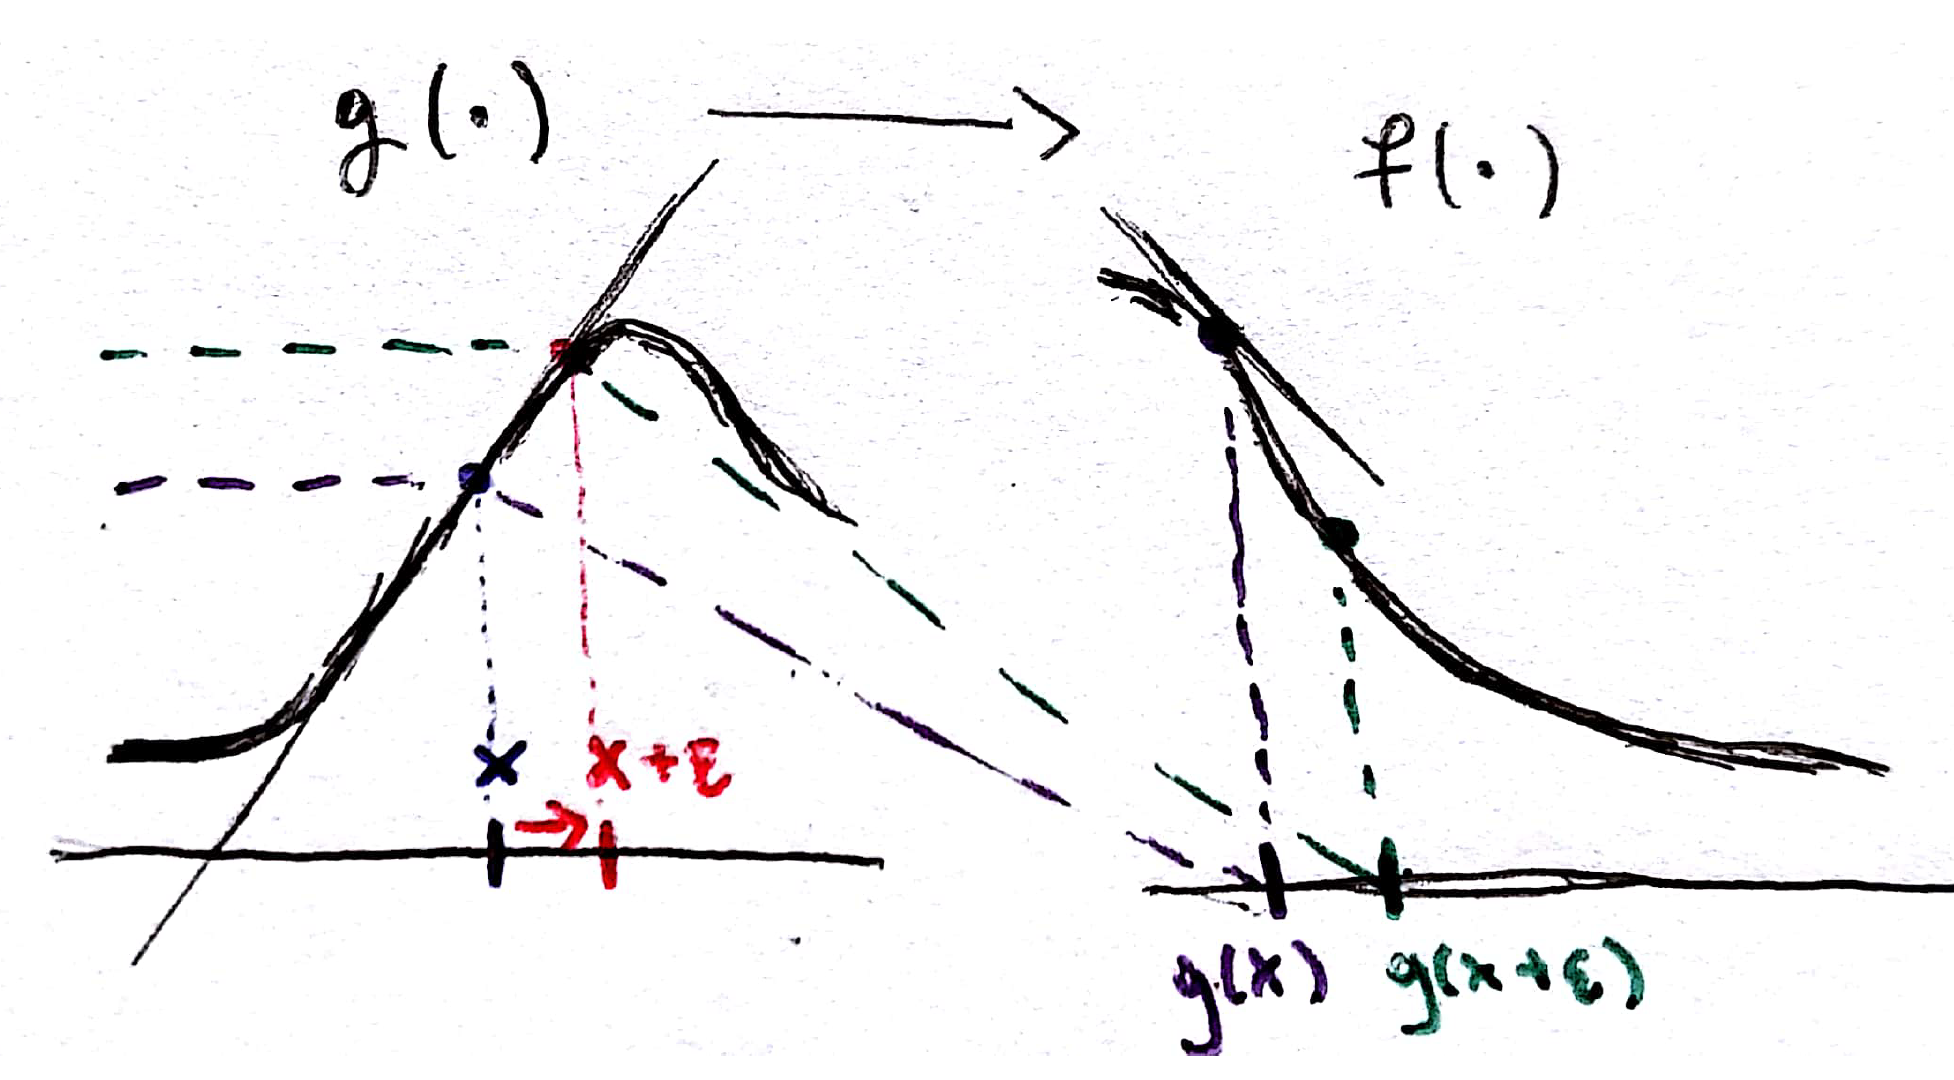
\includegraphics[width=0.75\paperwidth]{figure/chain_rule_2}
   \caption{The chain rule tells us how a small change in $x$ affects the
     downstream output of a composition of functions, in terms of the changes it
     causes within each intermediate function. \label{fig:chain_rule_2} }
 \end{figure}
\end{frame}

\begin{frame}
  \frametitle{Review: The Chain Rule}
  \begin{itemize}
  \item Derivative of composition $\rightarrow$ multiplication of derivatives
    \begin{align*}
      D\left(f^{K} \circ f^{K - 1} \dots \circ f^{1}\right)\left(x\right) &= \left[\prod_{k = 2}^{K} D f^{k}\left(h_{k - 1}\right)\right]D f^1\left(x\right)
    \end{align*}
    where $h_k = f^{k}\left(h_{k - 1}\right)$ is output of previous level (and $h_0 = x$)
  \end{itemize}
  \begin{figure}[ht]
    \centering
    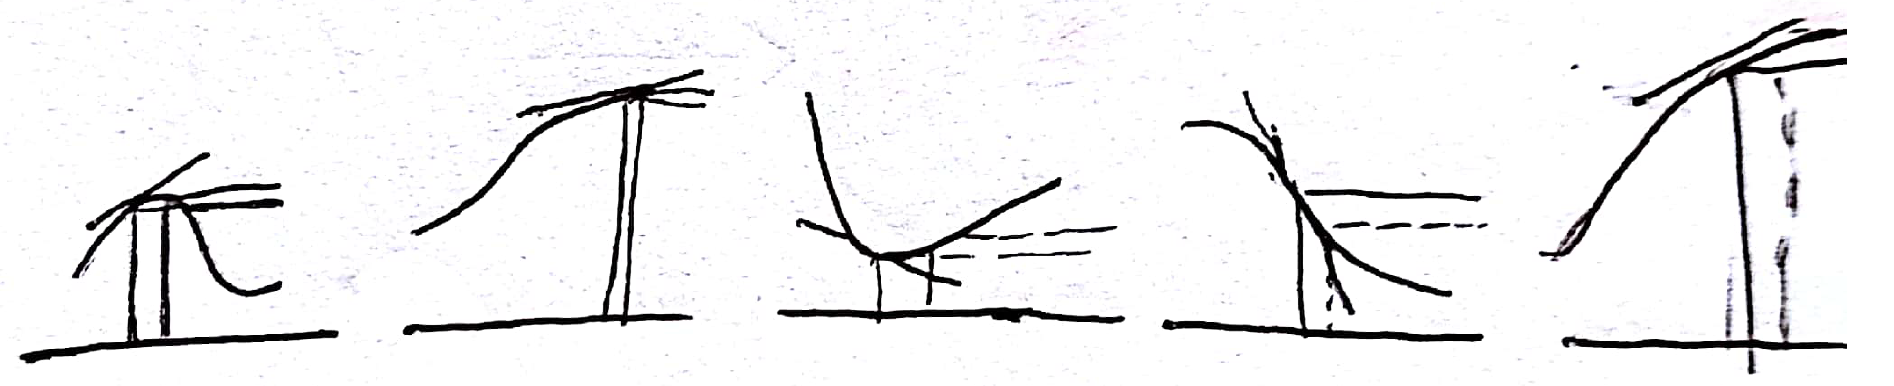
\includegraphics[width=0.8\paperwidth]{figure/chain_rule_k}
    \caption{The chain rule tells us how a small change in $x$ affects the
      downstream output of a composition of functions, in terms of the changes it
      causes within each intermediate function. \label{fig:chain_rule_k} }
  \end{figure}
\end{frame}

\begin{frame}
  \frametitle{Chain Rule for Logistic Regression}
  \begin{itemize}
  \item We can now find the derivative of the logistic regression loss much more
    elegantly
  \item Remember that it has these intermediate functions
    \begin{enumerate}
    \item $\ell\left(\sigma\right) = y_i\log\sigma + \left(1 - y_i\right)\log\left(1 - \sigma\right)$
    \item $\sigma\left(z\right) = \frac{1}{1 + \exp{-z}}$
    \item $\theta^{T}x_i$
    \end{enumerate}
  \item Their derivatives are (check this!)
    \begin{enumerate}
    \item $\frac{\partial}{\partial \sigma}\ell\left(\sigma\right) = \frac{y_i}{\sigma} - \frac{1 - y_i}{1 - \sigma}$
    \item $\frac{\partial}{\partial z}\sigma\left(z\right) = -\sigma\left(z\right)\left(1 - \sigma\left(z\right)\right)$
    \item $\nabla_{\theta} \theta^{T} x_i = x_i$
    \end{enumerate}
  \end{itemize}
\end{frame}

\begin{frame}
  \frametitle{Chain Rule for Logistic Regression}
  \begin{itemize}
  \item Multiply the derivatives and substitute input from the flow graph
  \item Gives the gradient,
    \begin{align*}
      &\left(\frac{y_i}{\sigma\left(\theta^{T}x_i\right)} - \frac{1 - y_i}{1 - \sigma\left(\theta^{T}x_i\right)}\right)\sigma\left(\theta^{T}x_i\right)\left(1 - \sigma\left(\theta^{T}x_i\right)\right)x_i \\
      = &\left[y_i\left(1 - \sigma\left(\theta^{T} x_i\right)\right) - \left(1 - y_i\right)\sigma\left(\theta^T x_i\right)\right]x_i \\
      = &\left(y_i - \pi_{\theta}\left(x_i\right)\right) x_i
    \end{align*}
    recalling that by definition $\pi_{\theta}\left(x_i\right) =
    \sigma\left(\theta^T x_i\right)$
  \item Nice interpretation: change $\theta$ a lot when $y_i$ is far from the
    prediction probability $\pi_{\theta}\left(x_i\right)$
  \end{itemize}
\end{frame}

\section{Representation Learning}

\begin{frame}
  \frametitle{Finding Meaningful Features}
 \begin{itemize}
 \item Want to estimate $p\left(y_i = \text{yak} \vert x_i\right)$
 \item Could use logistic regression if the input $x_i$ were meaningful
 \end{itemize}
 \begin{figure}[ht]
   \centering
   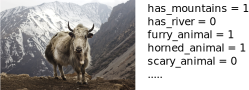
\includegraphics[width=0.7\paperwidth]{figure/image_features_ideal}
   \caption{It would be nice if our images came with qualitative annotation
     about what was in them. \label{fig:image_features_ideal} }
 \end{figure}
\end{frame}

\begin{frame}
  \frametitle{Finding Meaningful Features}
 \begin{itemize}
 \item Want to estimate $p\left(y_i = \text{yak} \vert x_i\right)$
 \item If our $x_i$'s are unstructured, this becomes much more difficult
 \item Logistic regression will fail
 \end{itemize}
 \begin{figure}[ht]
   \centering
   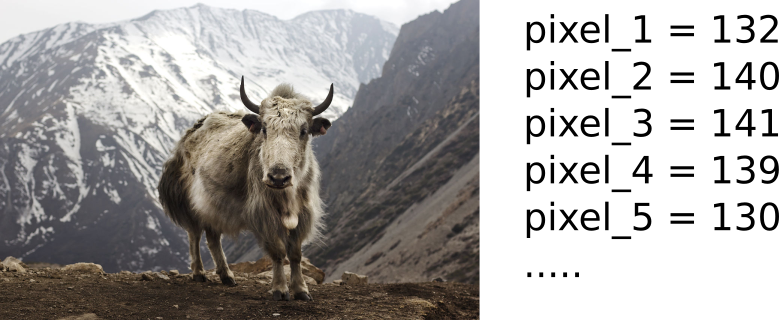
\includegraphics[width=0.7\paperwidth]{figure/image_features_reality}
   \caption{In reality, we can't manually provide all this
     annotation. \label{fig:image_features_reality} }
 \end{figure}
\end{frame}

\begin{frame}
  \frametitle{Finding Meaningful Features}
 \begin{itemize}
 \item If our $x_i$'s are unstructured, this becomes much more difficult
 \item Logistic regression will fail
 \end{itemize}
 \begin{figure}[ht]
   \centering
   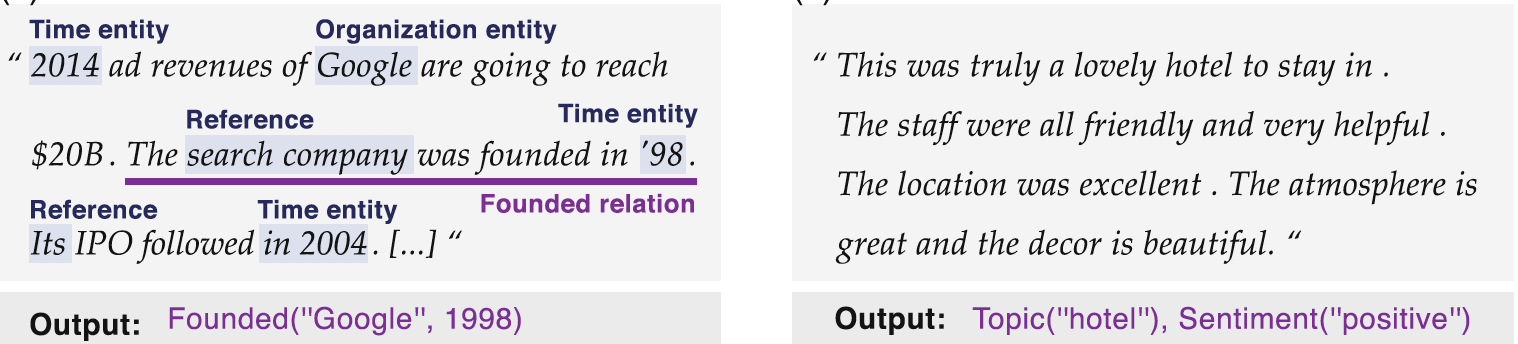
\includegraphics[width=0.7\paperwidth]{figure/language_features}
   \caption{Similarly, extracting meaningful structure from raw text would be
     useful in a variety of downstream tasks. \label{fig:language_features} }
 \end{figure}
\end{frame}

\begin{frame}
  \frametitle{Our Goal}
  \begin{itemize}
  \item Try to automatically learn meaningful features
  \item Start with simple features at low layers
  \item Increase feature complexity in a compositional way
  \end{itemize}
  \begin{figure}[ht]
    \centering
    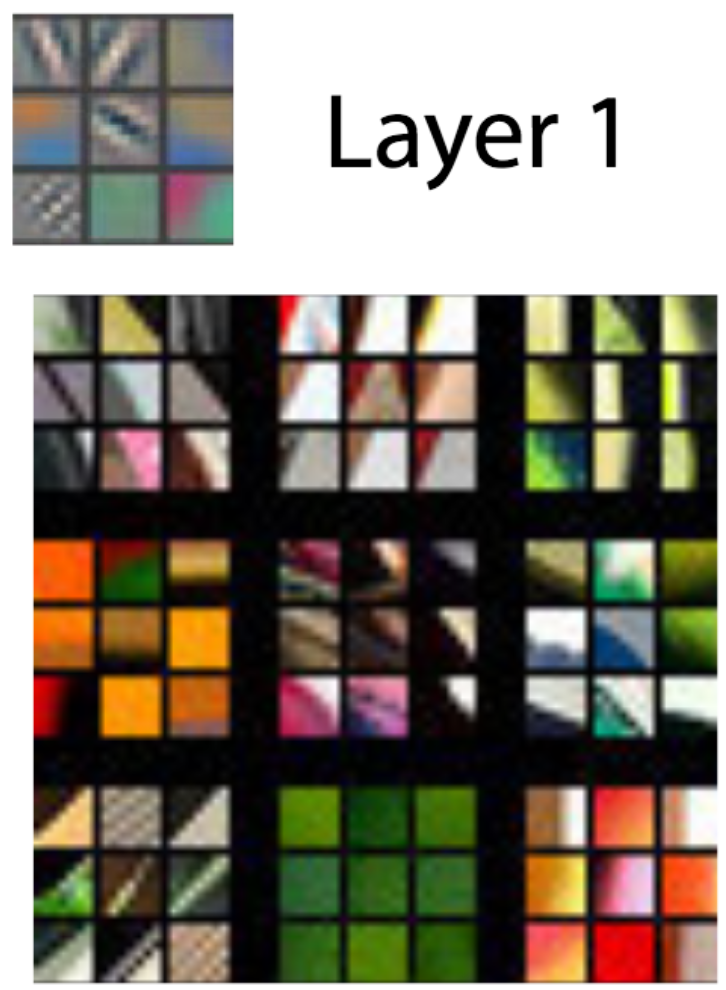
\includegraphics[width=0.3\paperwidth]{figure/zf_layer1}
    \caption{Early layers might create features corresponding to edges of
      different orientations. \label{fig:zf_layer1} }
  \end{figure}
\end{frame}

\begin{frame}
  \frametitle{Our Goal}
  \begin{itemize}
  \item Try to automatically learn meaningful features
  \item Start with simple features at low layers
  \item Increase feature complexity in a compositional way
  \end{itemize}
  \begin{figure}[ht]
    \centering
    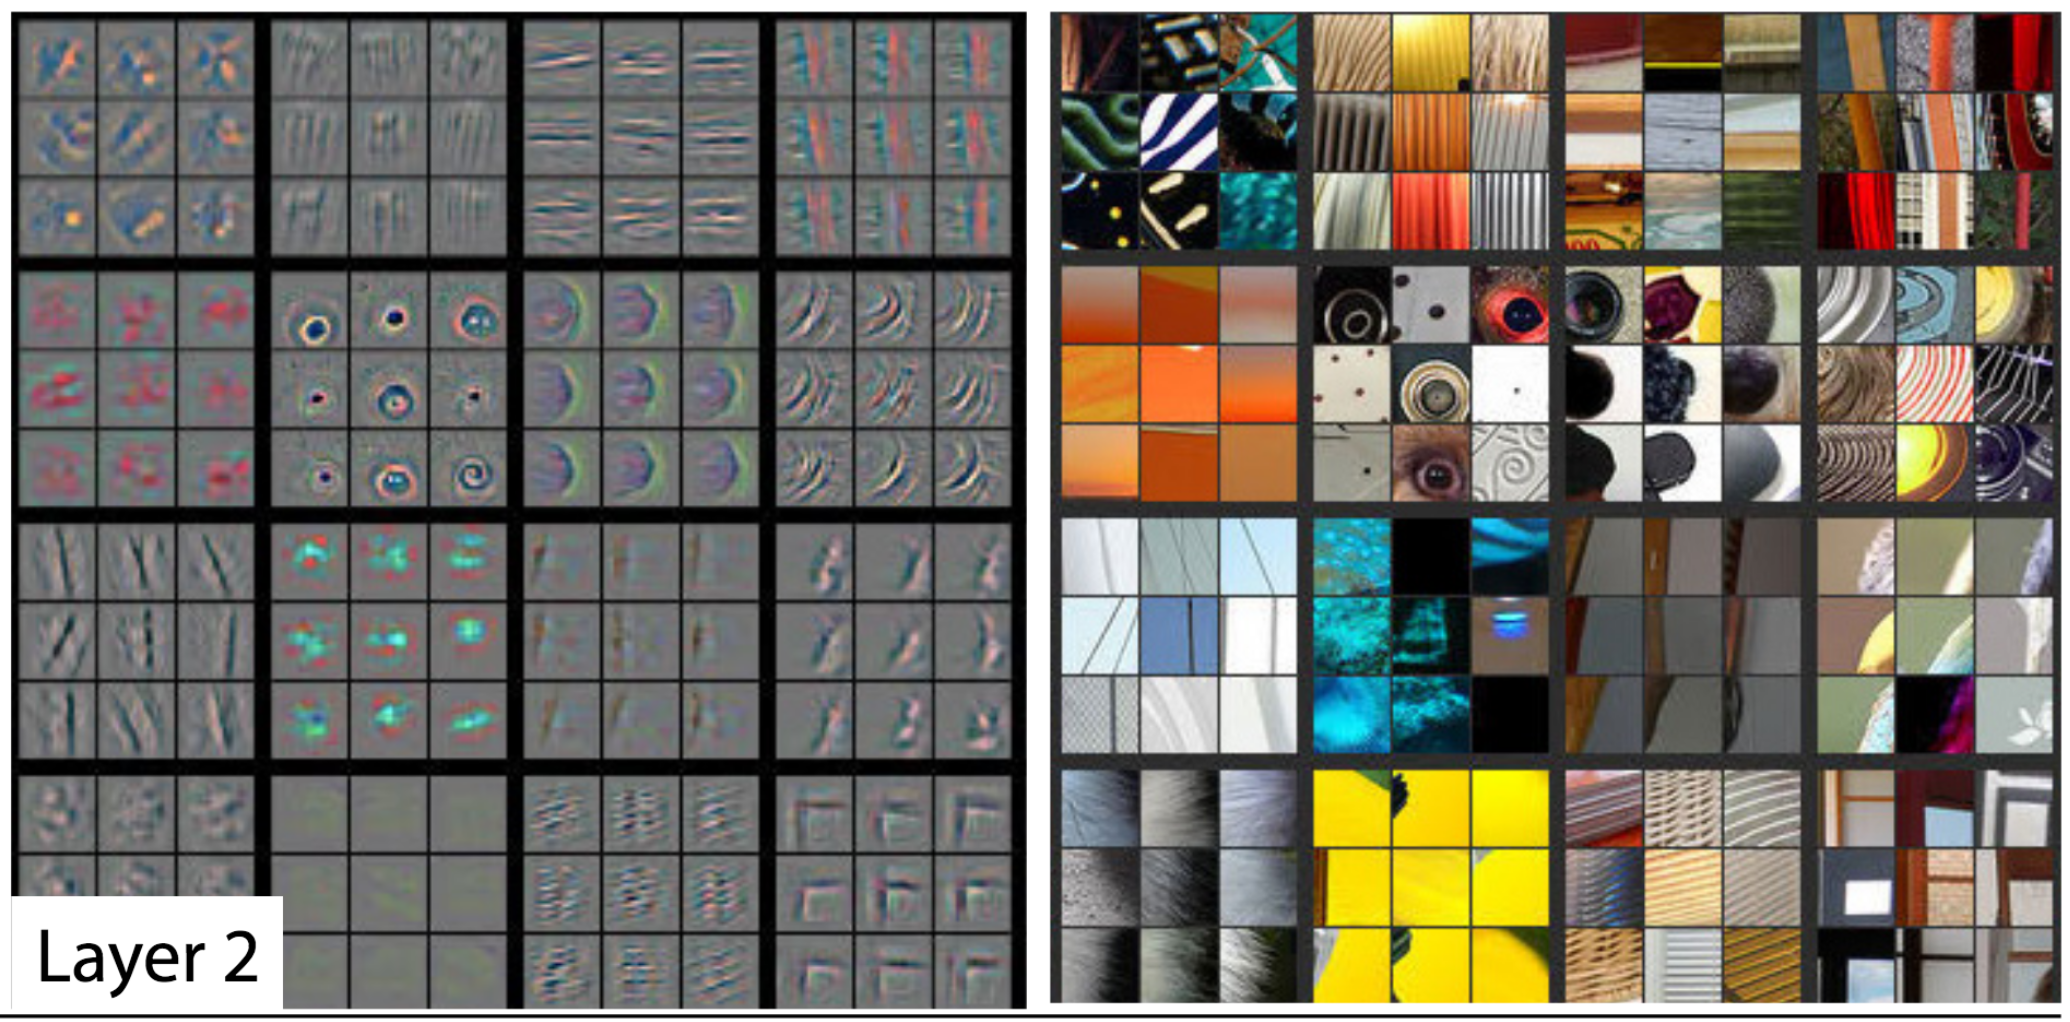
\includegraphics[width=0.7\paperwidth]{figure/zf_layer2}
    \caption{Features increase in complexity as you get deeper in the
      network. \label{fig:zf_layer2} }
  \end{figure}
\end{frame}

\begin{frame}
  \frametitle{Our Goal}
  \begin{itemize}
  \item Try to automatically learn meaningful features
  \item Start with simple features at low layers
  \item Increase feature complexity in a compositional way
  \end{itemize}
  \begin{figure}[ht]
    \centering
    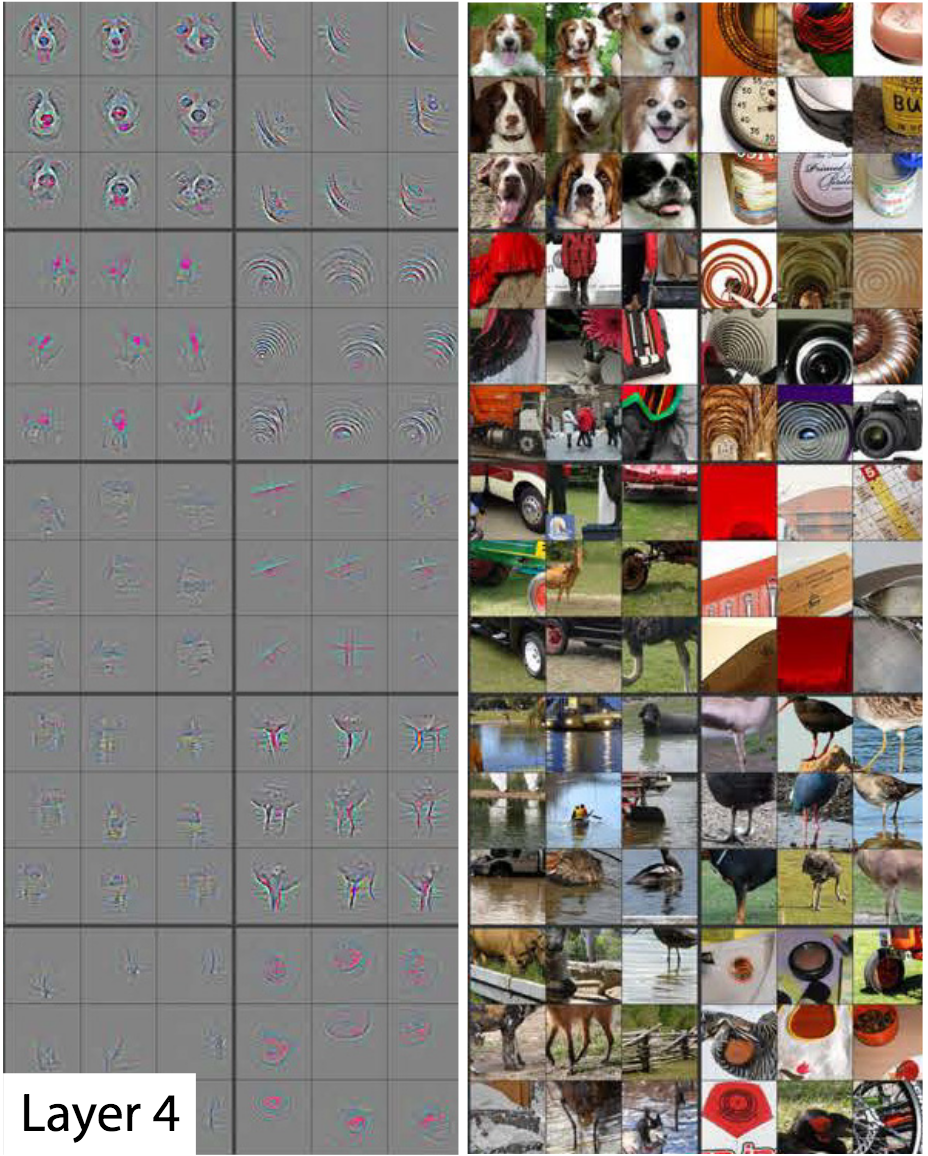
\includegraphics[width=0.3\paperwidth]{figure/zf_layer4}
    \caption{Eventually we will have meaningful high-level features.
      \label{fig:zf_layer4} }
  \end{figure}
\end{frame}

\begin{frame}
  \frametitle{Our Goal}
  \begin{itemize}
  \item Try to automatically learn meaningful features
  \item Start with simple features at low layers
  \item Increase feature complexity in a compositional way
  \end{itemize}
  \begin{figure}[ht]
    \centering
    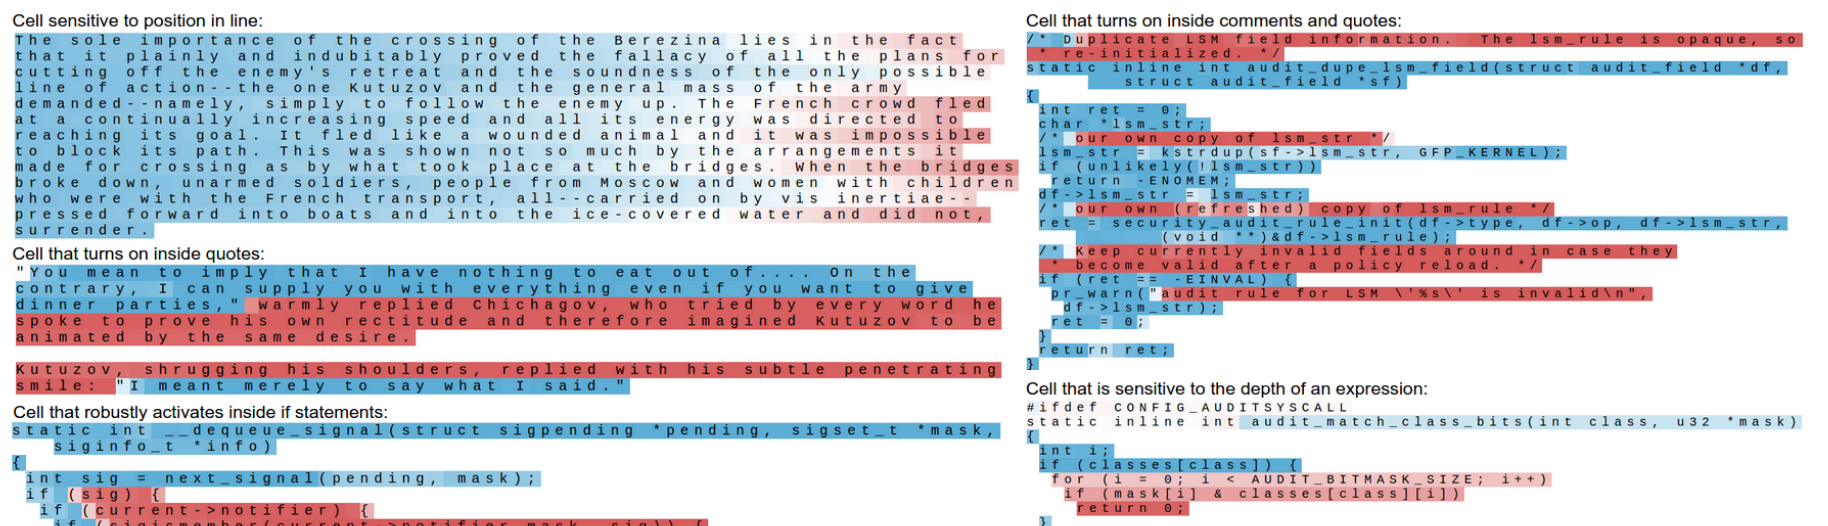
\includegraphics[width=0.8\paperwidth]{figure/high_layer_text}
    \caption{Similar kinds of complex features can emerge in text applications
      too.
      \label{fig:layer_text} }
  \end{figure}
\end{frame}

\begin{frame}
  \frametitle{Mixing \& Stacking Logistic Regressions}
  \begin{itemize}
    \item Simple combinations of simple functions quickly become complex
    \item These complex compositions could capture meaningful features
  \end{itemize}
  \begin{figure}
    \centering
    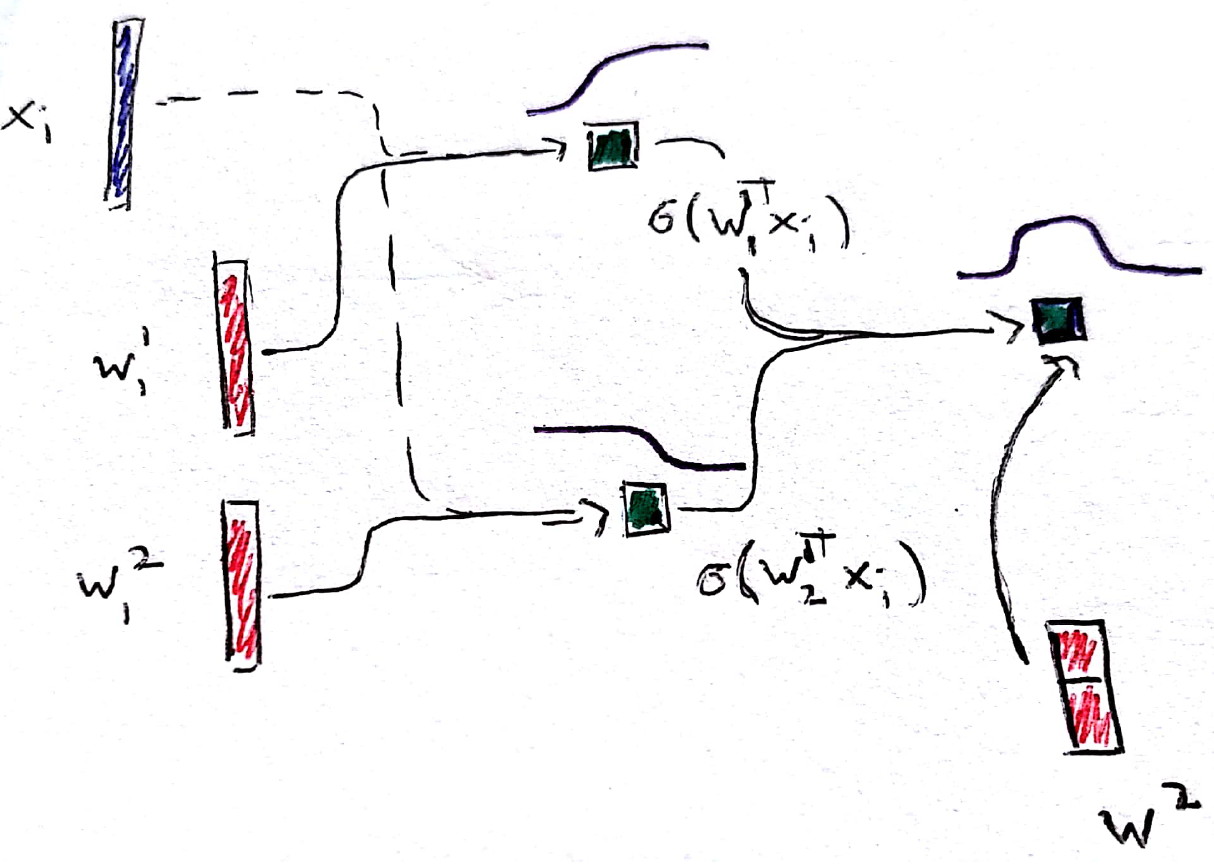
\includegraphics[width=0.55\paperwidth]{figure/mixture_logistic_2}
    \caption{Simply mixing two logistic regressions, we can represent
      nonmonotonic functions. \label{fig:mixture_logistic_2} }
  \end{figure}
\end{frame}

\begin{frame}
  \frametitle{Discussion}
  \begin{itemize}
  \item Which of the following functions \textit{cannot} be represented by the
    mixture of two logistic regressions?
  \item Can you think of other functions that cannot be learned this way?
  \end{itemize}
  \begin{figure}[ht]
    \centering
    \includegraphics[width=0.5\paperwidth]{figure/mlog_discuss}
  \end{figure}
\end{frame}

\begin{frame}
  \frametitle{Mixing \& Stacking Logistic Regressions}
  \begin{itemize}
  \item Simple combinations of simple functions can quickly become complex
  \item These complex compositions could capture meaningful features
  \end{itemize}
  \begin{figure}
    \centering
    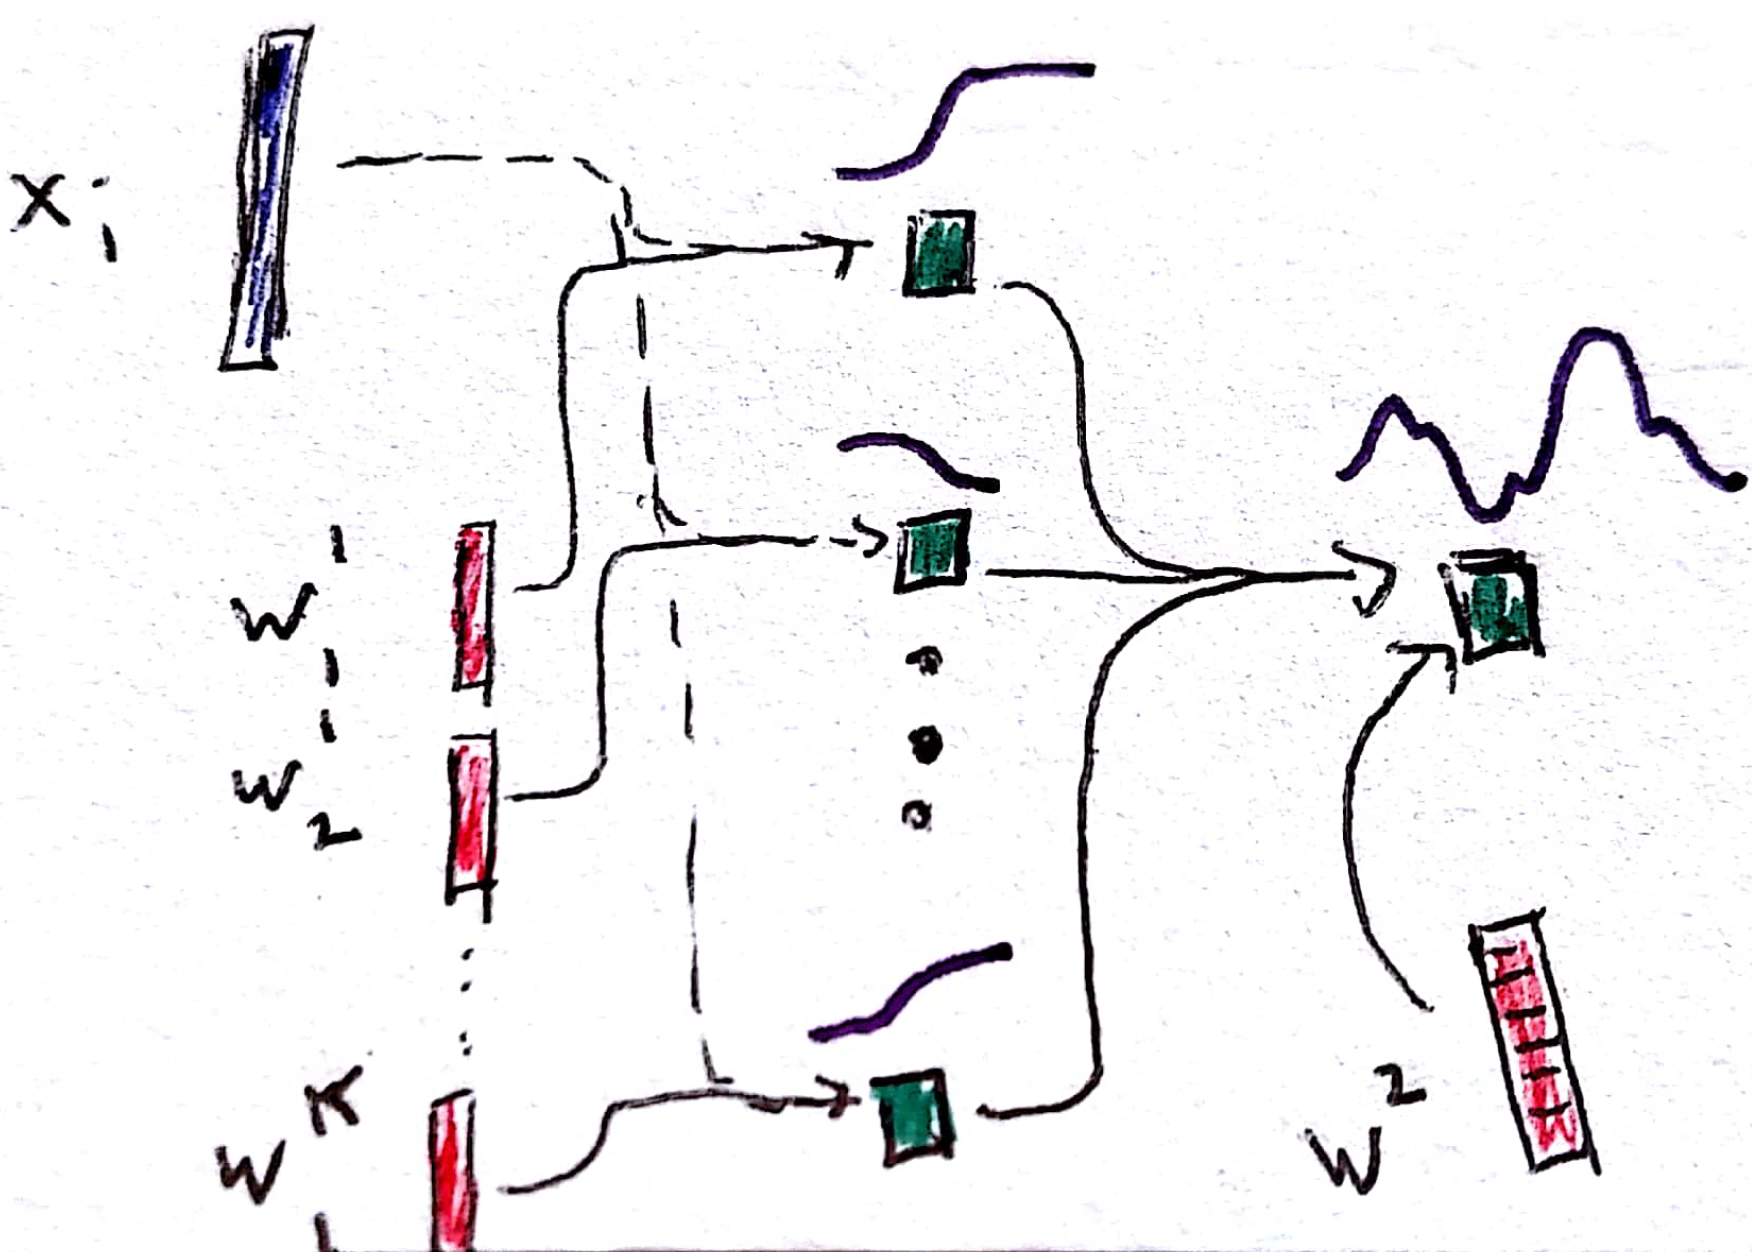
\includegraphics[width=0.55\paperwidth]{figure/mixture_logistic_k}
    \caption{Mixing more sigmoids, we can represent even more complicated
      functions. \label{fig:mixture_logistic_k} }
  \end{figure}
\end{frame}

\begin{frame}
  \frametitle{Mixing \& Stacking Logistic Regressions}
  \begin{itemize}
  \item New notation: Representation at layer $k$,
    \begin{align*}
      h_{k} = f^k\left(h_{k - 1}; W_k\right) \stackrel{\text{defined}}{=} \sigma\left(W_k h_{k - 1}\right)
    \end{align*}
  \end{itemize}
  \begin{figure}
    \centering
    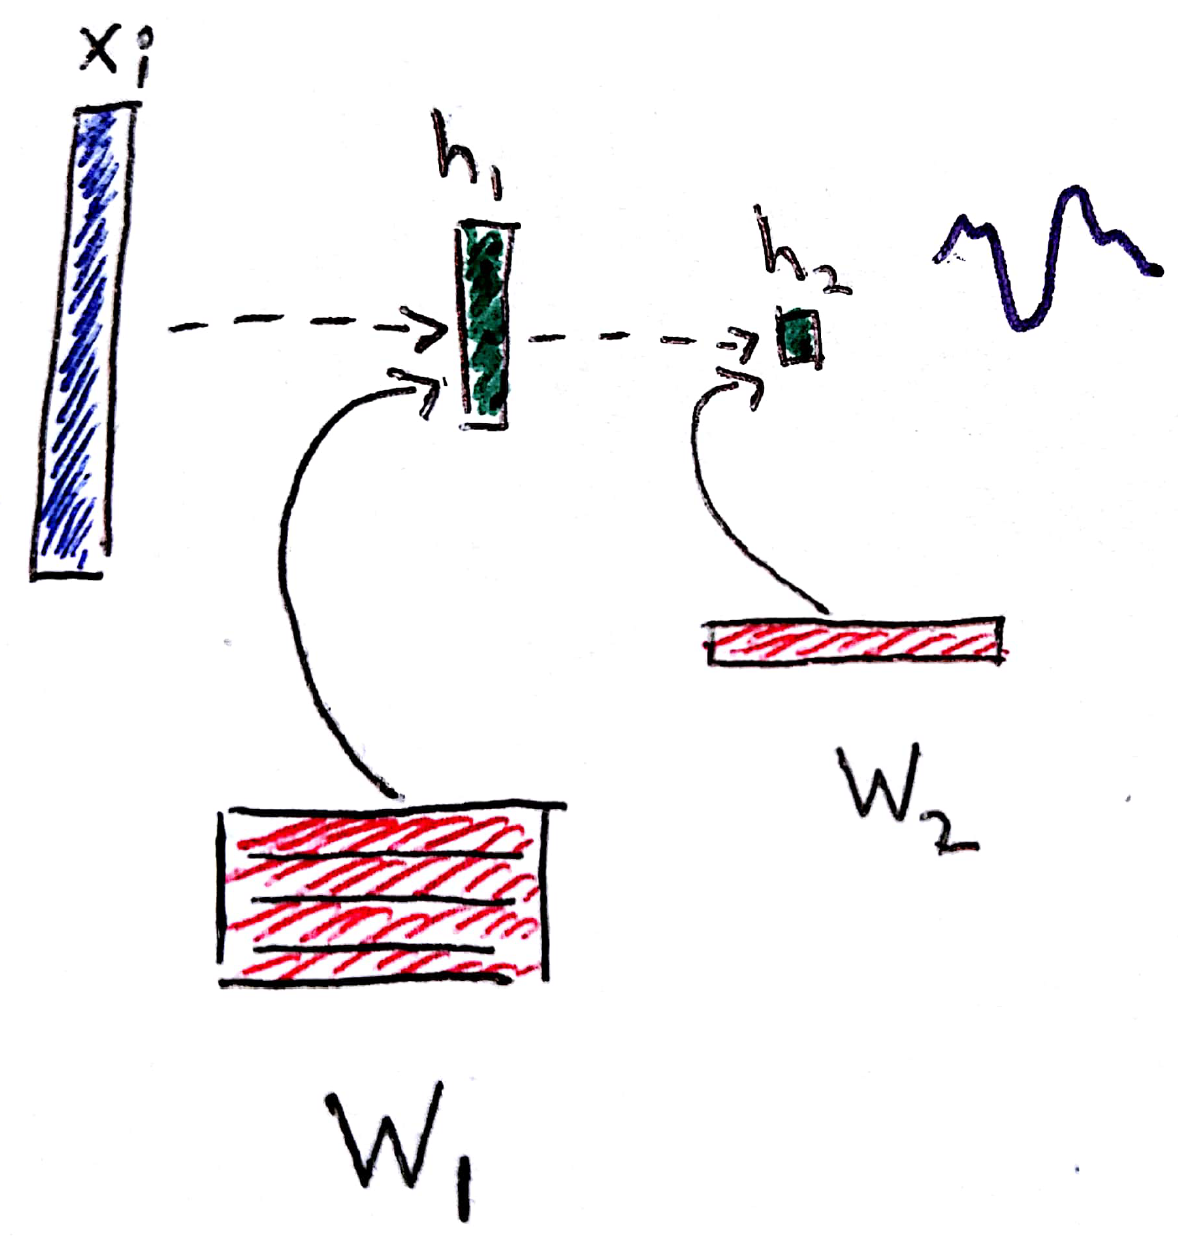
\includegraphics[width=0.4\paperwidth]{figure/mixture_logistic_k_stacked}
    \caption{Mixing more sigmoids, we can represent even more complicated
      functions. \label{fig:mixture_logistic_k_block} }
  \end{figure}
\end{frame}

\begin{frame}
  \frametitle{Mixing \& Stacking Logistic Regressions}
  \begin{itemize}
  \item New notation: Representation at layer $k$,
    \begin{align*}
      h_{k} = f^k\left(h_{k - 1}; W_k\right) \stackrel{\text{defined}}{=} \sigma\left(W_k h_{k - 1}\right)
    \end{align*}
  \end{itemize}
  \begin{figure}
    \centering
    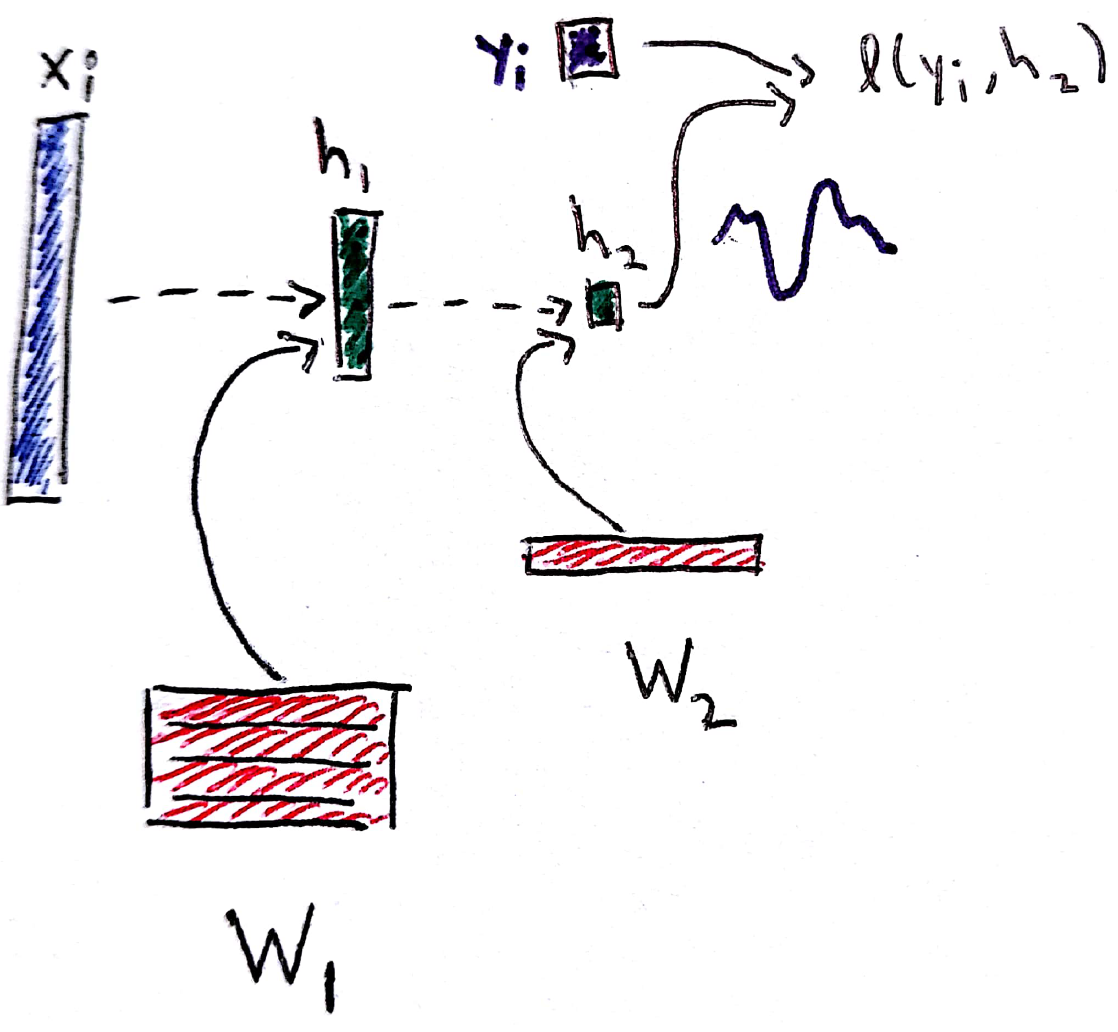
\includegraphics[width=0.4\paperwidth]{figure/mixture_logistic_k_stacked_loss}
    \caption{Mixing more sigmoids, we can represent even more complicated
      functions. \label{fig:mixture_logistic_k_block} }
  \end{figure}
\end{frame}

\begin{frame}
  \frametitle{Mixing \& Stacking Logistic Regressions}
  \begin{itemize}
  \item Simple combinations of simple functions can quickly become complex
  \item These complex compositions could capture meaningful features
  \end{itemize}
  \begin{figure}
    \centering
    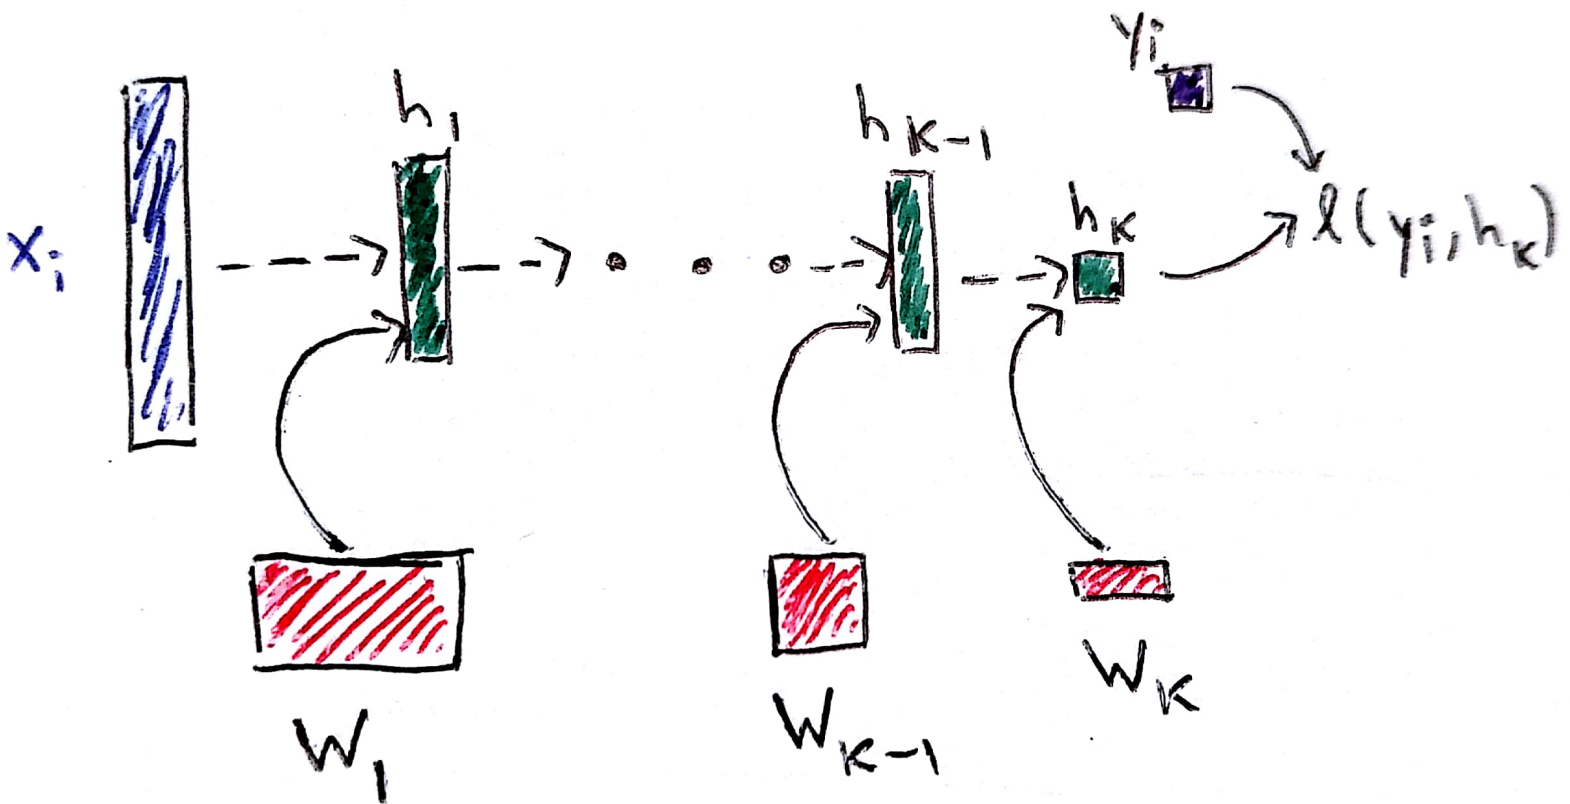
\includegraphics[width=0.7\paperwidth]{figure/deep_learning_basic}
    \caption{The basic idea of deep learning is to compose nonlinearities in a
      way that encourages discovery of complex intermediate representations
      $h_k$.
      \label{fig:deep_learning_basic} }
  \end{figure}
\end{frame}

\begin{frame}
  \frametitle{Aside: Activations}
  \begin{itemize}
  \item For nonlinearity, we used sigmoid
  \item Many types of nonlinearities can be used instead
  \item The basic idea of mixing together simple functions remains the same
  \item Most common these days are Rectified Lienar Unites (ReLUs)
    \begin{itemize}
    \item They are easier to optimize (alleviate vanishing gradient problem)
    \end{itemize}
  \end{itemize}
\begin{figure}[ht]
  \centering
    \begin{subfigure}{0.16\paperwidth}
      \centering
      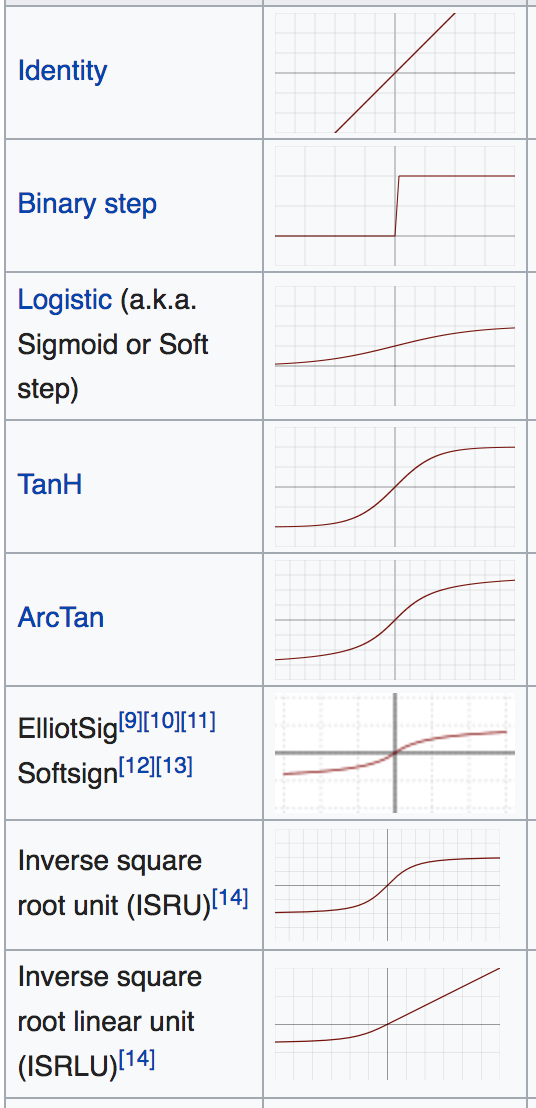
\includegraphics[width=0.16\paperwidth]{figure/activation_examples_1}
    \end{subfigure}
    \begin{subfigure}{.16\paperwidth}
      \centering
      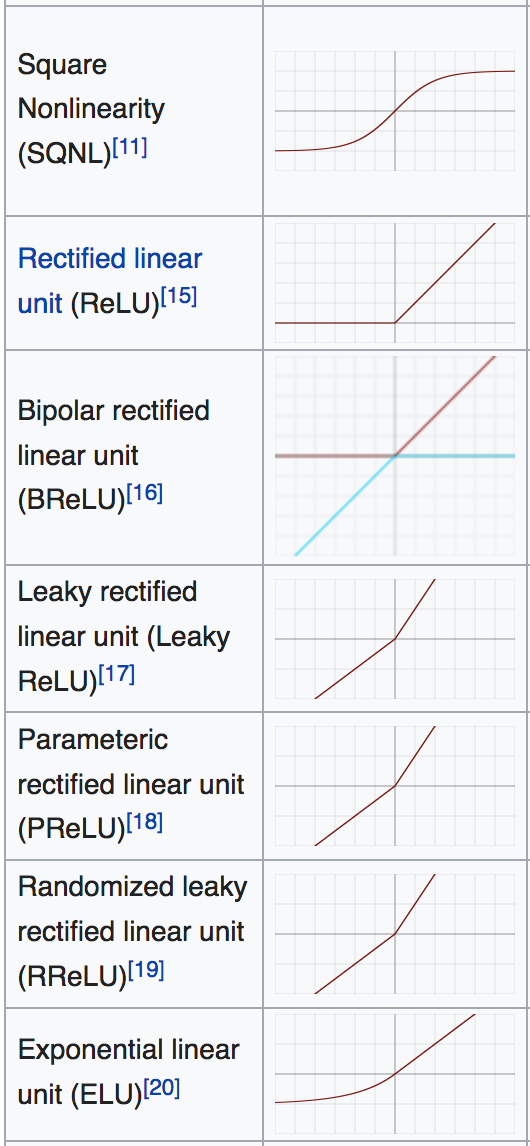
\includegraphics[width=0.16\paperwidth]{figure/activation_examples_2}
    \end{subfigure}
  \caption{\label{fig:activations} Some example nonlinearities from
    \url{https://en.wikipedia.org/wiki/Activation_function}. }
\end{figure}
\end{frame}

\section{Optimization}
\label{sec:optimization}


\begin{frame}
  \frametitle{Optimization: Stochastic Gradient Descent}
  \begin{itemize}
  \item Optimize by moving in a direction expected to decrease loss
  \item SGD: Estimated direction of gradient, after looking at small batch of
    data
  \item These days, other methods used too -- Adam, AdaGrad, AdaDelta, ...
  \end{itemize}
\begin{figure}[ht]
  \centering
  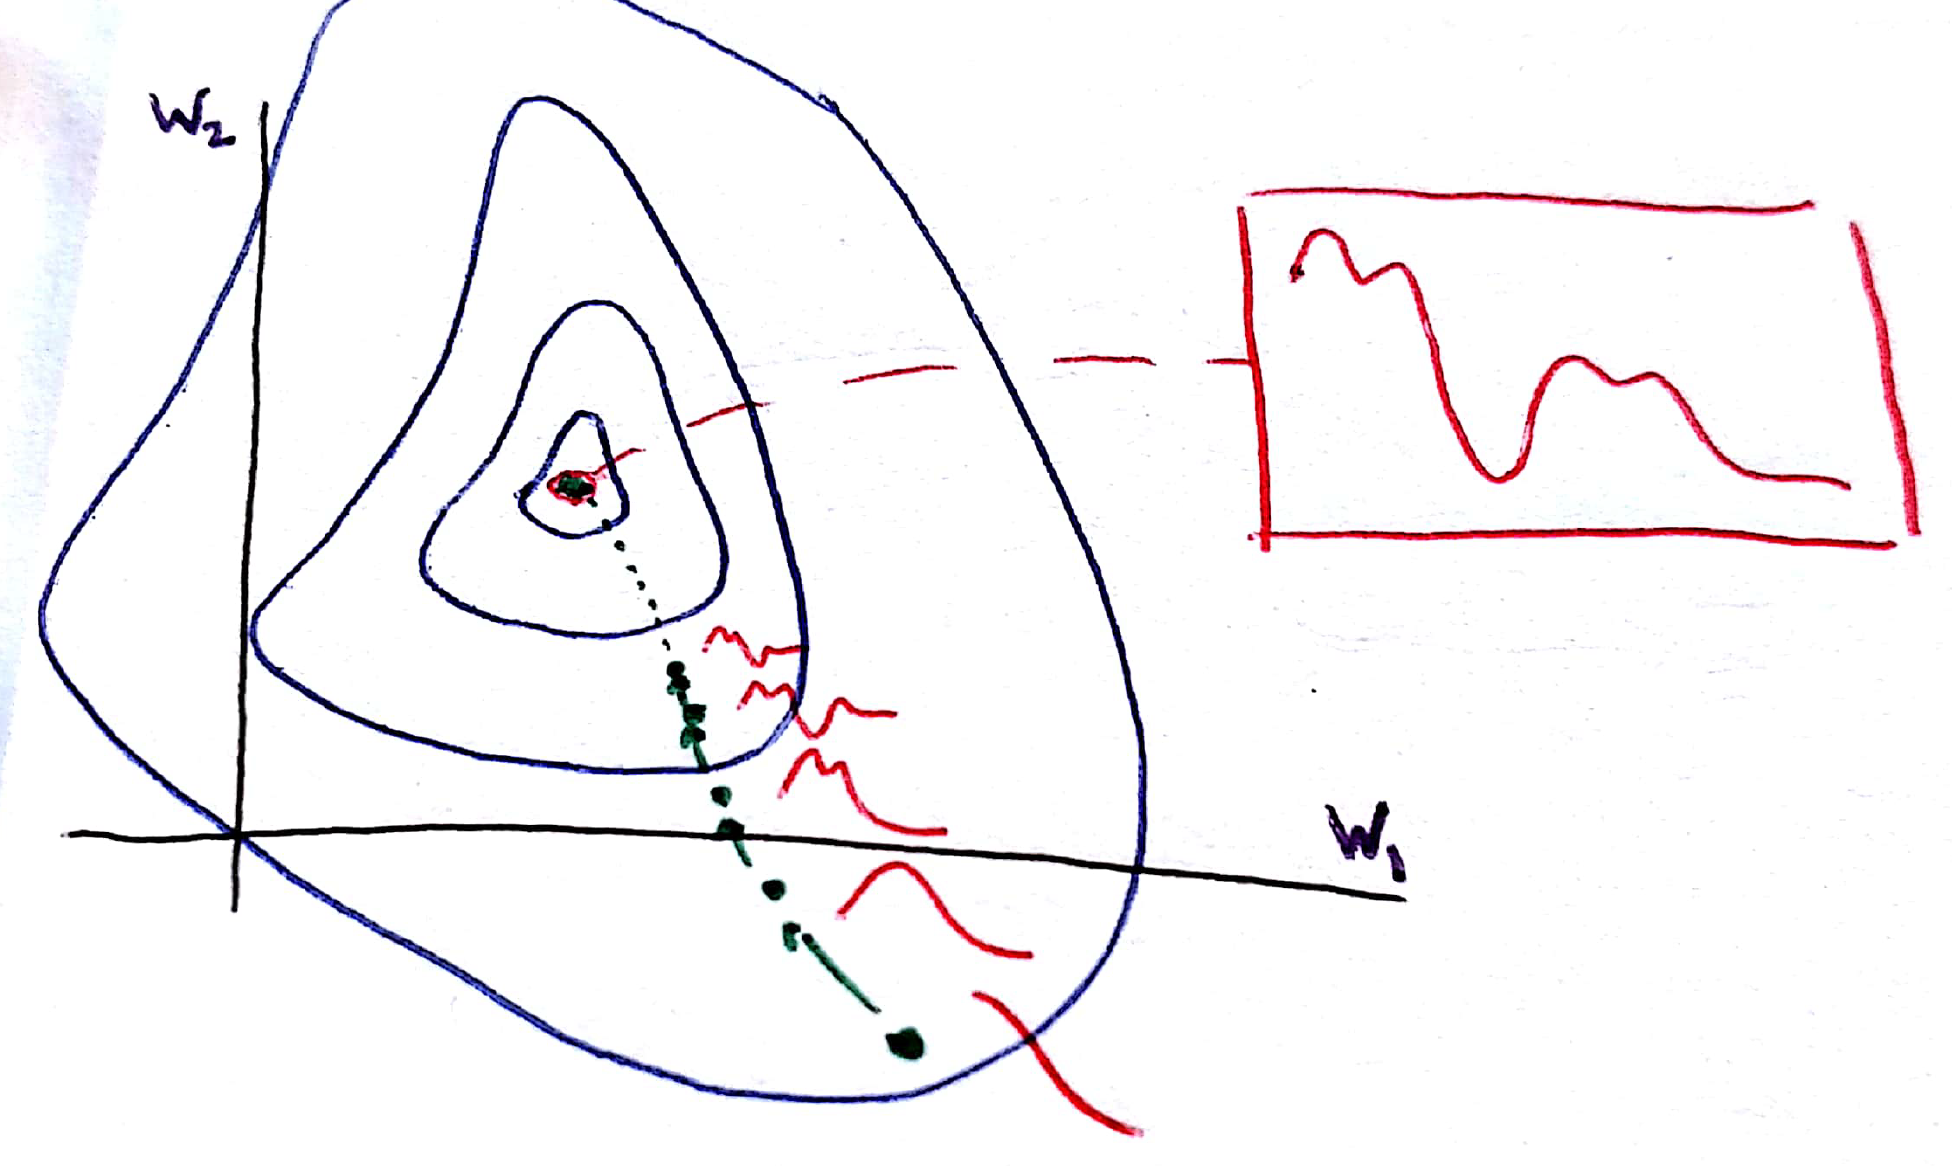
\includegraphics[width=0.6\paperwidth]{figure/sgd_example}
  \caption{Each optimization step modifies model parameters to make the fitted
    function closer ot the true (local) minimizer of the loss.
    \label{fig:sgd_example} }
\end{figure}
\end{frame}

\begin{frame}
  \frametitle{Backpropagation via Flow Graphs}
  \begin{itemize}
  \item For each iteration of SGD, we need to estimate the gradient of the loss
    with respect to the parameters
  \item When you perturb $W_k$ a little, it changes all the downstream $h_k, h_{k +
    1}, \dots, h_{K}$ up to the prediction, which uses that final representation
  \item There is a lot of composition going on here... courage alone won't help
    you take these derivatives
  \item Chain rule saves the day again!
  \end{itemize}
\end{frame}

\begin{frame}
  \frametitle{Chain Rule Revisited}
  \begin{itemize}
  \item Chain rule for vector-valued transformations $x \xrightarrow{g} h
    \xrightarrow{f} y$,
    \begin{align*}
      D\left(f \circ g\right)\left(x\right) &= Df\left(h\right)Dg\left(x\right)
    \end{align*}
  \end{itemize}
  \begin{figure}[ht]
    \centering
    \begin{subfigure}{0.2\paperwidth}
      \includegraphics[width=0.2\paperwidth]{figure/layer_flow}
    \end{subfigure}
    \begin{subfigure}{0.7\paperwidth}
      \includegraphics[width=0.7\paperwidth]{figure/chain_rule_matrices}
    \end{subfigure}
    \caption{The first row shows the sequence of vector-valued transformations.
      The $ij^{th}$ cell of the derivative matrices tells you how the $i^{th}$
      output changes when you perturb the $j^{th}$ input
      slightly. \label{fig:chain_rule_matrices} }
  \end{figure}
\end{frame}

\begin{frame}
  \frametitle{Flow Graphs}
  \begin{itemize}
  \item A flow graph shows how different vectors are computed from one another
    \begin{itemize}
    \item Nodes are vectors
    \item Edges are specific operations on input, which when combined with other
      incoming edges gives the output
    \end{itemize}
  \item Crucial: Operations along each edge should be easily differentiable with
    respect to input
  \end{itemize}
\begin{figure}[ht]
  \centering
  \includegraphics[width=0.2\paperwidth]{figure/flow_graph}
  \caption{The main idea of a flow graph. \label{fig:flow_graph} }
\end{figure}
\end{frame}

\begin{frame}
  \frametitle{Chain Rule on Graphs}
  \begin{itemize}
  \item When differentiating function $f_i$ with respect to upstream $h_k$, the
    chain rule implies
    \begin{align*}
      Df_{i}\left(h_k\right) &= \sum_{j \in C\left(i\right)}
      Df_{i}\left(h_{j}\right)Dh_{j}\left(h_{i}\right)
    \end{align*}
  \end{itemize}
  \begin{figure}[ht]
    \centering
    \includegraphics[width=0.4\paperwidth]{figure/graph_chain_rule}
    \caption{The graph version of the chain rule sums over the immediate
      children, referring recursively to similar gradients.
       \label{fig:flow_graph} }
  \end{figure}
\end{frame}

\begin{frame}
  \frametitle{Argument for Formula}
  \begin{itemize}
  \item This may look unfamiliar, but it's really the earlier matrix product in
    disguise
  \item Consider the case where we conceptually split $h$ into $h^{1}$ and
    $h^{2}$
  \end{itemize}
  \begin{figure}[ht]
    \centering
    \includegraphics[width=0.3\paperwidth]{figure/fg_intuition2}
    \caption{If we are splitting $h$, we can split all the derivatives in the
      matrix product. \label{fig:fg_intuition1} }
  \end{figure}
\end{frame}

\begin{frame}
  \frametitle{Argument for Formula}
  \begin{itemize}
  \item This may look unfamiliar, but it's really the earlier matrix product in
    disguise
  \item Consider the case where we conceptually split the intermediary $h$ into
    $h^{1}$ and $h^{2}$
  \end{itemize}
  \begin{figure}[ht]
    \centering
    \includegraphics[width=0.5\paperwidth]{figure/fg_intuition1}
    \caption{If we are splitting $h$, we can split all the derivatives in the
      matrix product. This can be written exactly as a sum, as in the earlier
      formula. \label{fig:fg_intuition1} }
  \end{figure}
\end{frame}

\begin{frame}
  \frametitle{Organized Gradient Computation}
  \begin{align*}
    Df_{i}\left(h_k\right) &= \sum_{j \in C\left(i\right)}
    Df_{i}\left(h_{j}\right)Dh_{j}\left(h_{i}\right)
  \end{align*}
  \begin{itemize}
  \item This gives a natural way of organizing gradient computation
  \item Start with output nodes and flow back towards inputs
  \item Remember each edge w.r.t input is straightforwards
  \end{itemize}
  \begin{figure}[ht]
    \centering
    \includegraphics[width=0.3\paperwidth]{figure/organized_comp1}
    \caption{Organization of computation to get gradients with respect to all
      inputs. \label{fig:organized_comp1} }
  \end{figure}
\end{frame}

\begin{frame}
  \frametitle{Organized Gradient Computation}
  \begin{align*}
    Df_{i}\left(h_k\right) &= \sum_{j \in C\left(i\right)}
    Df_{i}\left(h_{j}\right)Dh_{j}\left(h_{i}\right)
  \end{align*}
  \begin{itemize}
  \item This gives a natural way of organizing gradient computation
  \item Start with output nodes and flow back towards inputs
  \item Remember each edge w.r.t input is straightforwards
  \end{itemize}
  \begin{figure}[ht]
    \centering
    \includegraphics[width=0.27\paperwidth]{figure/organized_comp2}
    \caption{Organization of computation to get gradients with respect to all
      inputs. \label{fig:organized_comp2} }
  \end{figure}
\end{frame}

\begin{frame}
  \frametitle{Organized Gradient Computation}
  \begin{align*}
    Df_{i}\left(h_k\right) &= \sum_{j \in C\left(i\right)}
    Df_{i}\left(h_{j}\right)Dh_{j}\left(h_{i}\right)
  \end{align*}
  \begin{itemize}
  \item This gives a natural way of organizing gradient computation
  \item Start with output nodes and flow back towards inputs
  \item Remember each edge w.r.t input is straightforwards
  \end{itemize}
  \begin{figure}[ht]
    \centering
    \includegraphics[width=0.3\paperwidth]{figure/organized_comp3}
    \caption{Organization of computation to get gradients with respect to all
      inputs. \label{fig:organized_comp3} }
  \end{figure}
\end{frame}

\begin{frame}
  \frametitle{Organized Gradient Computation}
  \begin{align*}
    Df_{i}\left(h_k\right) &= \sum_{j \in C\left(i\right)}
    Df_{i}\left(h_{j}\right)Dh_{j}\left(h_{i}\right)
  \end{align*}
  \begin{itemize}
  \item This gives a natural way of organizing gradient computation
  \item Start with output nodes and flow back towards inputs
  \item Remember each edge w.r.t input is straightforwards
  \end{itemize}
  \begin{figure}[ht]
    \centering
    \includegraphics[width=0.3\paperwidth]{figure/organized_comp4}
    \caption{Organization of computation to get gradients with respect to all
      inputs. \label{fig:organized_comp3} }
  \end{figure}
\end{frame}

\begin{frame}
  \frametitle{Consequence: Backpropagation}
  \begin{itemize}
  \item The flow graph for a standard deep neural net is straightforwards
  \end{itemize}
  \begin{figure}[ht]
    \centering
    \includegraphics[width=0.6\paperwidth]{figure/layer_flow_graph}
    \caption{The flow of computation within a single layer. \label{fig:layer_flow_graph} }
  \end{figure}
\end{frame}

\begin{frame}
  \frametitle{Modularity}
  \begin{itemize}
  \item Gradients make use only of \textit{local} information
  \item Can propose arbitrary new layers, as long as you can define gradient of
    output with respect to input
  \item Has let people experiment widely in literature,
    \begin{itemize}
    \item Convolution layers \citep{lecun1995convolutional}
    \item Attention mechanisms \citep{olah2016attention}
    \item LSTM cells \citep{schmidhuber1997long}
    \item Residual layers \citep{he2016deep}
    \item ...
    \end{itemize}
  \item And all sorts of mixing and matching between these
  \end{itemize}
\end{frame}

\section{Debugging Deep Learning}

\begin{frame}
  \frametitle{Hyperparameter Tuning}
  \begin{itemize}
  \item Deep learning models can be hard to train
  \item Depending on various hyperparameters,
    \begin{itemize}
    \item Sequence of (per-layer) learning rates
      \begin{itemize}
      \item Other optimization parameters (e.g., momentum)
      \end{itemize}
    \item Type, number, and width of each layer
    \item Batch size
    \item Regularization
    \item Weight initialization
    \item Activation functions
    \item Preprocessing (e.g., standardization, PCA, or quantile transformation)
    \end{itemize}
    the model may or may not train properly
  \end{itemize}
\begin{figure}[ht]
  \centering
    \begin{subfigure}{.2\paperwidth}
      \centering
      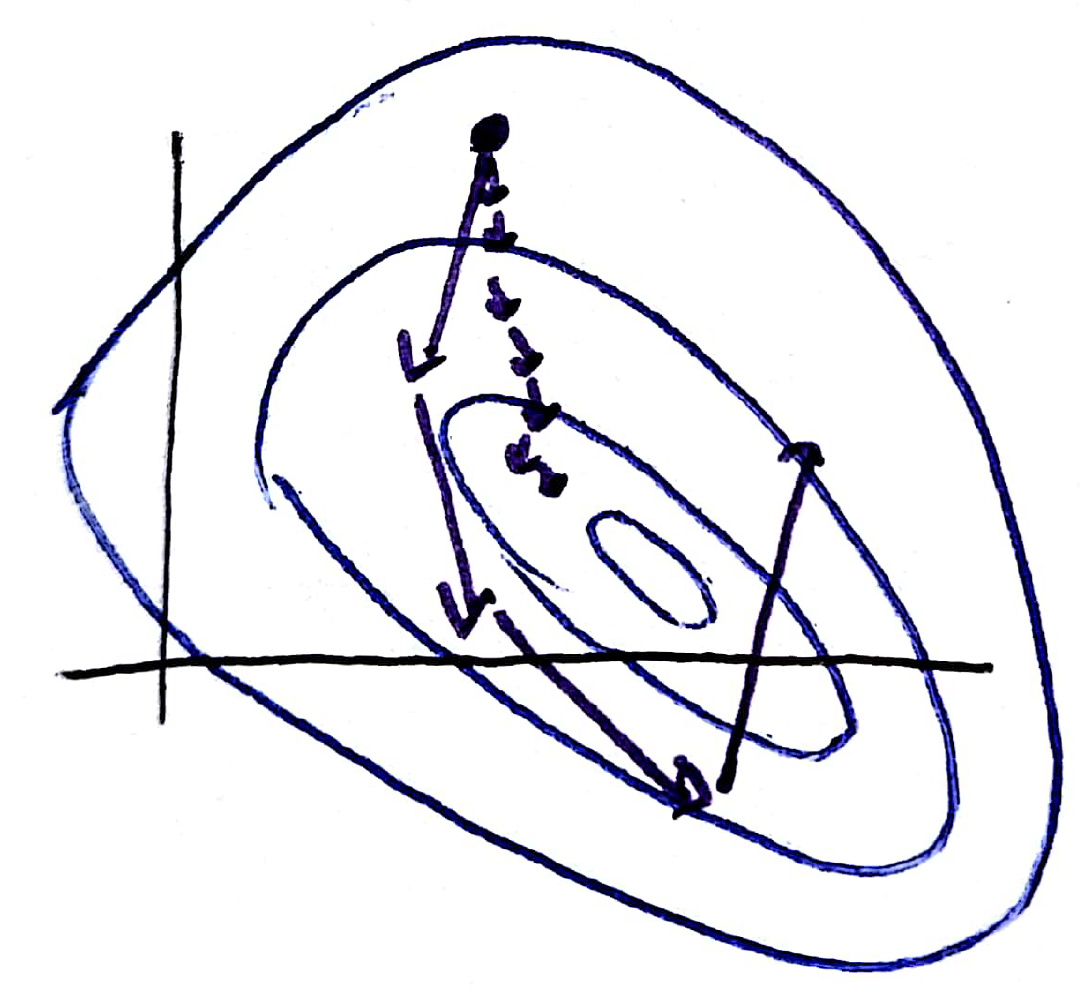
\includegraphics[width=0.17\paperwidth]{figure/learning_rate_effect}
    \end{subfigure}
    \begin{subfigure}{.2\paperwidth}
      \centering
      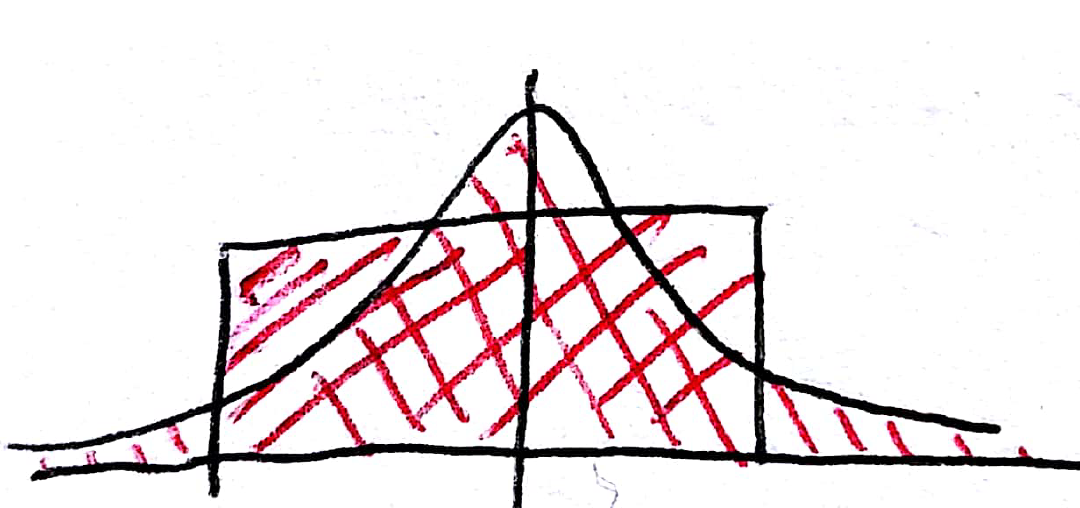
\includegraphics[width=0.17\paperwidth]{figure/weight_initialization}
    \end{subfigure}
    \begin{subfigure}{.2\paperwidth}
      \centering
      \includegraphics[width=0.17\paperwidth]{figure/architecture_choice}
    \end{subfigure}
    \caption{Three types of hyperparameters that can affect training: Those
      associated with optimization, regularization of the loss, and model
      architecture.
    \label{fig:hyperparameters} }
\end{figure}
\end{frame}

\begin{frame}
  \frametitle{Search Strategy}
  \begin{itemize}
  \item Multiresolution search: Coarse exploration followed by detailed
    investigation
  \item Semi-automated strategy: Analyze simple sweeps, launch new jobs
    accordingly
  \item Alternatives to grid search: Search in random grid, or use Bayesian
    Optimization
  \item Cheap validation alternatives: Instead of full training in all
    experiments, use cheap proxies
  \end{itemize}
  \begin{figure}[ht]
    \centering
    \includegraphics[width=0.6\paperwidth]{figure/random_search}
    \caption{A comparison of grid and random search, from
      \citep{bergstra2012random}. \label{fig:random_search} }
  \end{figure}
\end{frame}

\begin{frame}
  \frametitle{Search Strategy}
  \begin{itemize}
  \item Multiresolution search: Coarse exploration followed by detailed
    investigation
  \item Semi-automated strategy: Analyze simple sweeps, launch new jobs
    accordingly
  \item Alternatives to grid search: Search in random grid, or use Bayesian
    Optimization
  \item Cheap validation alternatives: Instead of full training in all
    experiments, use cheap proxies
  \end{itemize}
  \begin{figure}[ht]
    \centering
    \includegraphics[width=0.4\paperwidth]{figure/freeze_thaw}
    \caption{An example of freeze-thaw bayesian optimization, from
      \citep{swersky2014freeze}. \label{fig:random_search} }
  \end{figure}
\end{frame}

\begin{frame}
  \frametitle{Training Analysis}
  \begin{figure}[ht]
    \centering
    \includegraphics[width=0.7\paperwidth]{figure/bias_variance}
    \caption{Typical strategy is to try to first overfit the model, then
      regularize to ensure validation performance. \label{fig:bias_variance} }
  \end{figure}
\end{frame}

\begin{frame}
  \frametitle{Exercise}
  Discuss the bias-variance tradeoffs associated with these training parameters
  \begin{itemize}
    \item Number and widths of layers
    \item Learning rates
    \item Number of iterations
  \end{itemize}
\end{frame}

\begin{frame}
  \frametitle{Training Analysis}
  \begin{itemize}
  \item It can be helpful to collect statistics
    \begin{itemize}
    \item Gradients
    \item Activation values
    \end{itemize}
  \item Save your model at checkpoints! Helps both debugging and restarting
    training
  \end{itemize}
  \begin{figure}[ht]
    \centering
    \begin{subfigure}{.5\paperwidth}
      \centering
      \includegraphics[width=0.4\paperwidth]{figure/activation_evolution}
    \end{subfigure}
    \begin{subfigure}{.5\paperwidth}
      \centering
      \includegraphics[width=0.4\paperwidth]{figure/backprop_histogram}
    \end{subfigure}
    \caption{Detective work to understand failures in training, from
      \citep{glorot2010understanding}.\label{fig:detective_work} }
  \end{figure}
\end{frame}

\begin{frame}
  \frametitle{Training Analysis}
  Other (more sophisticated) forms of visualization that can be useful,
  \begin{itemize}
  \item Study low-dimensional representation of function as it trains
  \item Vary subset of weights for a given example, see how maps change
  \end{itemize}
  Many, many more ideas in \citep{bengio2012practical}.
\begin{figure}[ht]
  \centering
  \includegraphics[width=0.4\paperwidth]{figure/pretraining_example}
  \caption{The model may be invariant to certain transformations of the
    parameters, but you can directly visualization a dimensionality reduction
    done on the functions over the course of training, as discussed in
    \citep{erhan2010does}. \label{fig:pretraining_example} }
\end{figure}

\end{frame}

% I really dislike blogs that just show screenshots of network architectures or worse benchmarking results
% don't like just randomly survey arbitrary papers
\begin{frame}
  \frametitle{Philosophy for Learning Deep Learning}
  \begin{itemize}
  \item Don't ignore history!
    \begin{itemize}
    \item No need to keep up with every retweeted paper
    \item There were many creative people long before deep learning
    \end{itemize}
  \item Whenever you encounter a new algorithm or formula,
    \begin{itemize}
    \item Sketch a toy example (one-dimensional, binary instead of multiclass,
      discrete instead of continuous, ...)
    \item Draw picture of a toy example
    \item Try to plug in simple values (0, 1, $\pm \infty$ are good choices)
    \end{itemize}
  \item Genius is overrated
    \begin{itemize}
    \item First of all, there's stackoverflow
    \item No amount of natural talent can make up for dedicated effort
    \item You can't learn everything overnight, but it's a journey worth taking
    \end{itemize}
  \end{itemize}
\end{frame}

\begin{frame}[allowframebreaks]
  \bibliographystyle{plain}
    \bibliography{refs}
\end{frame}
\end{document}
